% hidelinks
% \documentclass[12pt,a4paper,twoside,openright]{scrreprt}
\documentclass[12pt,a4paper,twoside,openright]{report}

% basics
\usepackage[english]{babel}
\usepackage[utf8]{inputenc}
\usepackage[T1]{fontenc}
\usepackage{cmap} % allow copy paste from pdf
\usepackage{graphicx}
\usepackage{minted}
\usepackage[babel]{microtype}
\usepackage{mathtools}
\usepackage[hyphens]{url}
\usepackage[unicode]{hyperref}
\usepackage[math]{blindtext}
\usepackage[mode=text,group-minimum-digits=4,round-mode=places,round-precision=2]{siunitx}
\usepackage{csquotes}
\usepackage{tikz}
\usetikzlibrary{arrows.meta,fit,calc}
\usepackage{algorithm,algpseudocode,algorithmicx}
\usepackage{multirow, makecell, bigstrut, booktabs, float}
\usepackage{tabularx}
\usepackage{amsmath}
\usepackage{amssymb}
\usepackage{bytefield}

% \usepackage{listings}
% \usepackage{algpseudocode}
% \usepackage{listingsutf8}
% \usepackage{multirow}
% \usepackage{booktabs}
% \usepackage{longtable}
% \usepackage{float}
% \usepackage{caption}
% \usepackage{abstract}
% \usepackage{ccicons}
% \usepackage{tikz}
% \usepackage{tablefootnote}
% \usepackage{color}
% \usepackage{scrhack}
% \usepackage{array}
% \usepackage{fancyvrb}
% \usepackage{appendix}
% \usepackage[amsmath,hyperref]{ntheorem}

\usepackage[
    title={Implementing a parallel Points-To Analysis},
    author={Lukas Böttcher},
    type={Master Thesis},
    institute={Christian-Albrechts-Universität zu Kiel},
    course={Computer Science},
    examiner={Prof.\ Dr.\ Hans Mustermann},
    supervisor={Dipl.-Inf.\ Roman Tiker,\\Dipl.-Inf.\ Laura Stern,\\Otto Normalverbraucher,\ M.Sc.},
    startdate={2022-08-01},
    enddate={2023-01-16},
    language=english
]{scientific-thesis-cover}

% set up biblatex
\usepackage[
  backend       = biber,
  sortcites     = true,
  bibstyle      = alphabetic,
  citestyle     = alphabetic,
  giveninits    = true,
  useprefix     = false, %"von, van, etc." will be printed, too. See below.
  minnames      = 1,
  minalphanames = 3,
  maxalphanames = 4,
  maxbibnames   = 99,
  maxcitenames  = 2,
  natbib        = true,
  eprint        = true,
  url           = true,
  doi           = true,
  isbn          = true,
  backref       = true]{biblatex}
\bibliography{literatur}

% set up hyperref
\hypersetup{
    linktoc=all,
    bookmarksnumbered=true,
    bookmarksopen=true,
    bookmarksopenlevel=1,
    breaklinks=true,
    pdftitle={Masterarbeit},
    pdfstartview=Fit,
    pdfpagelayout=SinglePage,    
}

\newcommand{\listingautorefname}{Listing}
\newcommand{\algorithmautorefname}{Algorithm}

\begin{document}
\pagestyle{empty}
\Coverpage
\Affirmation
\cleardoublepage
\begin{abstract}
    Pointer analysis is a subgroup of static analysis techniques. 
    In general, the goal is to detect a set of memory locations for each pointer element in a program. 
    All major compiler systems make use of this information in order to optimize the given code during compilation
    and most importantly, to detect errors in the program.
    In this thesis an interprocedural inclusion-based pointer analysis, PTAGPU, is presented that utilizes the parallel execution of GPGPUs to speedup the pointer analysis as part of the SVF framework. 
    As the SVF framework itself is built on top of the LLVM compiler infrastructure, 
    it is possible to run the proposed analysis on any program that can be compiled inside the LLVM toolchain.
    A meaningful speedup was observed with the proposed parallel implementation compared to the single threaded highly optimized wave propagation inclusion-based pointer analysis.
    An evaluation of the proposed analysis is provided both through the SVF testsuite as well as a collection of open source programs used as benchmarks.
\end{abstract}
\cleardoublepage
\tableofcontents
\cleardoublepage
\listoffigures
\cleardoublepage
\listoftables
\cleardoublepage

\pagestyle{headings}
\chapter{Introduction} \label{chap:intro}
The goal of this thesis is the implementation of a parallel implementation of a pointer analysis. As well as researching to what extent such an implementation presents advantages or disadvantages over other analyses that are not strictly parallel in nature.

\section{Structure of this Thesis}
This thesis is divided into three chapters.
The first chapter \autoref{chap:intro} lays the groundwork for the implementation and goes into detail what ideas were persued in order to develop the implementation. All related current work and it's influences on this work is discussed here, as well as the motivation for the implementation itself. Furthermore the fundamentals of pointer analysis are explained here with code samples and an end to end analysis workflow that aims to illustrate the connection between actual code and its representation in a pointer analysis.

In the second chapter \autoref{chap:main} the software, namely PTAGPU, that was developed as part of this thesis, is described in detail. Design decisions, integrations with other software libraries and correctness are elaborated here.
The experimental benchmark results and how they wre generated are also presented here.

The last chapter \autoref{chap:conclusion} covers possible future work that could further improve the implementation and explore more ideas concerning parallel pointer analyses.
This chapter also discusses the experimental results from \autoref{chap:main}.


\section{Pointer Analysis}
In general a pointer analysis tries to find the values of pointers in a program at runtime, without having to execute the program.
So naturally this problem is undecidable \cite{landi1992undecidability} following a reduction from the halting problem.
As a result, performing a pointer analysis becomes a delicate balancing act between precision and peformance.
Commonly analyses produce over-approximation of the targets each pointer can point towards at runtime while other parts of an analyses might omit or under-approximate certaint parts for the sake of performance and scalability.
As a result, these analyses are strictly speaking unsound or soundy as put forward by \cite{livshits2015defense}:

\begin{quote}
    We introduce the term soundy for
    such analyses. The concept of soundiness
    attempts to capture the balance,
    prevalent in practice, of over-approximated
    handling of most language features, yet deliberately
    under-approximated handling of a feature subset well
    recognized by experts. Soundiness is in
    fact what is meant in many papers that
    claim to describe a sound analysis. A
    soundy analysis aims to be as sound as
    possible without excessively compromising
    precision and/or scalability.
\end{quote}

Pointer analyses build the foundation for a variety of other static analyses, since call-graph generation is directly dependent on pointer analysis in order to resolve indirect or dynamic calls statically.

One common pointer analysis is the inclusion-based Andersen's analysis \cite{andersen1994program}. The details of this type of analysis will be discussed later on, as it is the underlying basis for the proposed algorithm in \autoref{chap:main}. The Andersen algorithm sacrifices precision in favor of performance and achives an upper bound of $O(n^3)$ where n represents the number of pointer variables relevant to the analysis. This is known as the cubic bottleneck of general Andersen analysis \cite{mathiasen2021fine}.
This showcases the tradeoff that all non-theoretical pointer analyses have to make in oder to be applicable to real programs and avoid undecidability. Furthermore Andersen's analysis is a P-complete problem and is therefore not trivially parallelizable.

As a general abstraction, pointer analyses can be seen as complex graph problems where programs are interpreted as graphs with nodes representing variables and edges representing relations between nodes, such as memory allocations and assignments bewteen variables.
This allows us to make use of a large body of previous research concerning graph problems and transform the general analysis into a better defined mathematical problem.

Another analysis closely related to pointer analysis is alias analysis, where two pointers are said to alias if their points-to sets have an intersection. An alias analysis produces a set of relations over all nodes in the analysis graph where nodes can either \textbf{NotAlias}, \textbf{MayAlias} or \textbf{MustAlias}.
For two given nodes, $a$, $b$ and their points-to sets $pts(a)$ and $pts(b)$ the following constraints describe the relations.
$$a\ \textbf{NotAlias}\ b \iff \forall ptd \in pts(a) \colon ptd \notin pts(b)$$
$$a\ \textbf{MayAlias}\ b \iff \exists ptd \in pts(a) \colon ptd \in pts(b)$$
$$a\ \textbf{MustAlias}\ b \iff \forall ptd \in pts(a) \colon ptd \in pts(b)$$
Both pointer analysis, alias analysis, as well as points-to analysis are all terms commonly used interchangeably in literature \cite{hind2001pointer}. From now on pointer analysis will be used in this thesis to refer to this type of static analysis from which an alias relation can be derived based on the pointer information.

A motivating example for pointer analyses is the detection on memory leaks in programs.
This occurs when a memory location is allocated on the heap, for example with a call to malloc in glibc, and is not freed at a later stage in the program.
It is in the interest of the developer to find such faults as to not exhaust the computers memory during execution by repeatedly allocating memory in the heap without freeing previous allocations.
Finding such logical errors can be accomplished via a related static analysis called data-flow analysis, where each possible value at different stages of the program is calculated. Here pointer information is vital, as pointers can represent lateral movement of data trough the control flow of a program, independent of direct assignments and read operations. Ultimately almost all static analyses require some kind of information about pointers to fully determine the state of a program.
Aside from error detection such as memory leaks, optimizations are another aspect of compiler systems, where pointer information is important to achieve better results, see \autoref{lst:dataflow}.
More often than not the pointer information alone does not provide an immediate value to the compiler or analysis tool, instead other procedures build on top of this information to derive valuable information about a program.

\begin{listing}
    \begin{minted}{c}
    #include <stdlib.h>
    void *iter;
    iter = value;

    /* depending on the data at value's memory location 
    the loop might not be necessary */
    
    while(*iter)
    {
        complex_computation(iter);
    }
    \end{minted}
    \caption{Optimizations in a c program}
    \label{lst:dataflow}
\end{listing}

\subsection{Notions of Sensitivity in Pointer Analysis}
As previously established, a complete pointer analysis is undecidable.
For this reason there are various notions of sensitivity when talking about pointer analysis.
These notions represent a compromise between precision, scalability and complexity of the analysis.
Following, some of the more common sensitivity notions will be illustrated to differentiate the more complex analyses from the less complex analyses and explain the impact of these sensitivities on actual performance when analyzing a program.

\subsubsection{Field-sensitivity}

\begin{listing}
    \begin{minted}{c}
    int a;
    char b;
    struct Person {
        char *name;
        int *age;
    } p1, p2;
    p1.age = &a;
    p1.name = &b;
        \end{minted}
    \caption{Field-sensitivity by example}
    \label{lst:field}
\end{listing}

Field-sensitivity describes how the pointer analysis algorithm handles structures in the program.
Most programming languages that expose memory management to a developer, such as c, c++ and Rust, offer some form of structures to represent an object that internally holds multiple values where these values might be pointers, that reference memory locations.
If an analysis is field-sensitive, each field of each struct is represented in the analysis as an independent node that can point to unique memory locations, as long as the field can be statically determined during the analysis, see \autoref{lst:field}.
If the field of a struct can not be statically determined, for example because of an arithmetic operation that produces multiple possible results for the offset during runtime, it is common for field-sensitive pointer analyses to fallback to a field-insensitive mode for the specific struct, wherein all fields of the struct are merged into a single abstract object.
For the given example, \verb|p1.age| and \verb|p1.name| can point to different memory locations.
Alternatively a field-insensitive analysis does not differentiate between any fields of a given struct at any point of the analysis.
Therefore only two nodes are created to represent the struct, $p1.*$ and $p2.*$.
Another common alternative is field-base-sensitivity, where instead of omitting the individual fields of each struct, the fields of every struct are merged into a single instance of that struct.
As a result the Person structs, p1 and p2, would be represented as a single object with fields name and age, such that \verb|p1.age == p2.age| are represented by the same node in the analysis.

\subsubsection{Array-sensitivity}
Array-sensitivity is conceptually similar to field-sensitivity but often has different effects on the runtime of the analysis.
For a given array $int arr[100]$ an array-sensitivie analysis would model each entry of the array, \newline e.g. arr[0], arr[1], \dots, with a unique node, whereas an insensitive analysis would model the array as a single node.
Generally speaking arrays are often homogeneous data structures that can hold a vast amount of data, compared to structs which are often more compact as they model attributes instead of raw data.
Therefore array-sensitivity if often omitted from whole program analyses, while field-sensitivity is common among pointer analyses.

\subsubsection{Scope of the analysis}
When designing a pointer analysis one has to make a decision about how to handle external code that the program depends on.
Often times a programs transitive dependencies can dwarf the original code by several magnitudes in size \cite{toman2017taming}.
Even a basic Hello World program in Java transitively depends on 3000 classes \cite{kulkarni2016accelerating} from the Java standard library.
For this reason most analyses either ignore external library code during analysis, or stub the most relevant library calls during analysis, such as \verb|malloc| or \verb|free|.
This tradeoff is well worth it, as most interesting properties in pointer analysis do not originate in extenal libraries, but the actual program code that is written by the developer.
This does however not solve the problem of standard library code mutating the program state either via callbacks or mutation of values behind pointer arguments. Here, simply ignoring the external code during analysis would greatly decrease the accuracy of the analysis.
For this reason, a lot of research is being done to develop methods that alleviate some of the problems that arise from analyzing external dependencies of a given program. Caching incremental results during analysis seems to be one of the most promising methods thus far \cite{mcpeak2013scalable}, where instead of solving the pointer analysis problem from the top-down, the analysis begins at the bottom and builds summaries for functions incrementally until a result over the entire program is achieved. Hybrid approaches combining top-down and bottom-up analysis represent state of the art analysis methods in use by production static analysis tools, such as Coverity \cite{mcpeak2013scalable}.

\subsubsection{Interprocedural analysis}
Another aspect that greatly influences the precision of analyses is whether they are interprocedural or intraprocedural.
An intraprocedural analysis only analyzes each function in an isolated context and disregards any influences on other functions or global state.
Interestingly most compilers rely mostly on intraprocedural analysis for bug detection as it can be performed in parallel for each function independently and is in general much faster than interprocedural analysis.
The following example \ref{lst:intraprocedural} illustrates the shortcomings of only performing intraprocedural analysis. Essentially parameter passing especially of pointers is not taken into account properly for the calculation of points-to sets.
An interprocedural analysis overcomes these limitations by connecting parameters of functions and the arguments at the respective callsites as well as the resulting return values in the graph structure that is used to solve the pointer analysis.
Fundamentally an interprocedural analysis is related to another notion of sensitivity, context sensitivity, since every context sensitive analysis has to be interprocedural in order to capture the context of each function call \cite{lin2015alias}.

\begin{listing}
    \begin{minted}{c}
        int *manupulatePointer(int *ptr);
        int main() {
            int *a, *b;
            b = manupulatePointer(a);
            /* intraprocedural analysis is unable 
            to determine the state of a or b */
        }
    \end{minted}
    \caption{Limitations of intraprocedural analysis}
    \label{lst:intraprocedural}
\end{listing}

\subsubsection{Flow-sensitivity}
When one performs a flow-sensitive pointer analysis, this means that the analysis takes into account the control flow of the program when calculating point-to information.
As can be seen in \ref{lst:flowsens}, a flow-sensitive analysis is in general more precise than a flow-insensitive analysis. Meanwhile running a flow-sensitive analyis is also exponentially more expensive to compute as every step in a programs control flow carries its own state concerning points-to relations - especially when the control flow is complicated by complex conditional statements or recursive execution.
Although this problem can be slightly alleviated, by only condering program statements that manipulate pointers.
Using a flow-sensitive pointer analysis also generates must-alias relations, compared to the comparatively imprecise may-alias relations from a flow-insensitive pointer analysis.
Generating definitive information that two variables will unconditionally alias during runtime is very valuable when considering refactoring optimizations by a compiler.
While a sound may-alias analysis requires that no possible alias relations are missed, a sound must-alias analysis requires analogously that no spurious alias relations are reported. Both are respectively over- and under-approximations of the true points-to results.

\begin{listing}
    \begin{minted}{c}
        int *manupulatePointer(int *ptr);
        int main() {
            int a, b, *x; // x -> {}
            if (something())
                x = &a; // x -> {a}
            else
                x = &b; // x -> {a,b} ?
            manupulatePointer(x);
            /* a flow insensitive analysis computes 
            a points-to set {a,b} for x while in actuality 
            x = &b and x = &a are mutually exclusive statements
            during execution */
        }
    \end{minted}
    \caption{Flow-sensitivity by example}
    \label{lst:flowsens}
\end{listing}

\subsubsection{Context-sensitivity}
As previouly eluded to, context-sensitivity is directly related to interprocedural analyses, since it governs how call sites and called functions are interpreted during the analysis.
More specifically a centext-sensitive analysis tries to qualify variables both on the heap and stack with contextual information such that different contexts can be established, where for example points-to information for a variable differs, thus improving the precision of the analysis.
To achieve this context-sensitivity can be modeled by using call-sites and objects to differentiate qualify the context for variables \cite{smaragdakis2015pointer}. Depending on the programming language at hand, these methods can yield different precision. It has been established that object oriented languages like Java greatly benefit from object-sensitivity over call-site-sensitivity, while more procedural languages like C benefit from call-site-sensitivity.
While a context-sensitive analysis would in theory provide more precision and therefore decrease the average size of points-to sets, in practice most context-sensitive pointer analyses, when applied to sizeable codebases, quickly grow out of control as the analysis explodes in terms of running time and space requirements \cite{smaragdakis2014introspective}. In contrast, context-insensitive analyses anecdotally scale better than context-sensitive analyses.

\begin{listing}
    \begin{minted}{c}
        int *manupulatePointer(int *ptr);
        int main() {
            int a, b, *x;
            x = &a;
            manupulatePointer(x);
            x = &b;
            manupulatePointer(x);
            /* a context-sensitive analysis evaluates both
            calls to manupulatePointer as unique function calls
            since the context differs between both calls */
        }
    \end{minted}
    \caption{Context-sensitivity by example}
    \label{lst:contextsens}
\end{listing}

\subsection{Andersen's Analysis}
Andersen's analysis is an inclusion based interprocedural pointer analysis algorithm first proposed by \cite{andersen1994program} in 1994. It is a field-sensitive, context-insensitive and flow-insensitive analysis. 
The algorithm was one of the first constraint based algorithms introduced for pointer analysis. Since it is lacking constext- and flow-sensitivity, it is often used as a base algorithm which produced broad over estimations of the points-to data and is later refined by more precise algorithms which improve the quality of the data and remove false positives from the points-to information generated by Andersen's algorithm.
The underlying idea is that the Algorithm operates on a given program by converting statements from the program into mathematical constraints contained in a constraint graph.
These constraints can be classified into a few types which can be seen in \autoref{tab:ander}.
It is worth noting that in literatur the field-sensitivity aspect is often omitted from the definition of the Andersen analysis although it was included in the original specification.
As mentioned in \autoref{chap:intro} the complexity of Andersen's analysis grows exponentially with regards to the number of pointer variables in a program. The reason for this exponential growth, among other aspects, is the field-sensitivity. Depending on the structure of the code under analysis, field-sensitivity might play the most influential part in the analysis' complexity. This will be further expanded upon in \autoref{chap:main}. Ultimaltely this is the reason for specifically including field-sensitivity when discussing Andersen's analysis in this thesis.
During execution an Andersen style pointer analysis repeatedly applies the constraints until a point is reached where no more changes are applied to the constraint graph at which point the execution concludes and the points-to sets for each variable are returned.
\begin{table}
    \begin{center}
        \caption{Constraints of an inclusion-based pointer analysis.}
        \label{tab:ander}
        \begin{tabular}{l|l|c|l}
            \hline                                                                                                                         \\
            \textbf{Statement} & \textbf{Name} & \textbf{Description}                        & \textbf{Constraint}                         \\
            \hline                                                                                                                         \\
            $x = \&a$          & alloca        & The address of a is assigned to variable x. & $\{a\} \subseteq pts(x)$                    \\
            $x = y$            & copy          & Variable y is assigned to x.                & $pts(y) \subseteq pts(x)$                   \\
            $x = *y$           & load          & Load value of y and assign to x.            & $\forall p \in pts(y) \colon p \subseteq pts(x)$ \\
            $*x = y$           & store         & Store y into value of x.                    & $\forall p \in pts(x) \colon y \subseteq pts(p)$ \\
            $x = y.f$          & field         & Field f of variable y is assigned to x      & $pts(y.f) \subseteq pts(x)$                 \\
        \end{tabular}
    \end{center}
\end{table}

\subsection{Steensgard's Analysis}
Steensgard's analysis was introduced in 1996 by \cite{steensgaard1996points}. It was inspired by Andersen's analysis and as such is also an interprocedural pointer analysis.
The key proposition of Steensgard's work was to improve the runtime of Andersen's algorithm by using equalities instead of subsets for the constraints that are used as inputs for the algorithm, an overview for the constraints can be seen in \autoref{tab:steens} - the rules are nearly identical to the constraints for the Andersen algorithm.
The change from subsets to equalities leads to an almost linear algorithm by utilizing union/find data structures for efficient computation of a fixpoint solution for a given set of pointers.
The tradeoff for this faster algorithm is precision, since Steensgard's algorithm quickly looses precicion compared to Andersen's algorithm by loosing the small differences between points-to sets of individual varialbes by equating them. An example for this precision loss can be seen in \autoref{lst:steensvander}.

\begin{listing}
    \begin{minted}{c}
        int main() {
            int a, b, *x, *y;
            x = &a; // pts(x) = {a}
            y = &b; // pts(y) = {b}
            y = x; // pts(y) = pts(x) = {a,b}
            /* by equating the points-to sets of x and y
            the fact that x never points to b is lost
            this leads to an obvious loss of precision */
        }
    \end{minted}
    \caption{Steensgard easily looses precision.}
    \label{lst:steensvander}
\end{listing}

\begin{table}
    \begin{center}
        \caption{Constraints of an equality-based pointer analysis.}
        \label{tab:steens}
        \begin{tabular}{l|l|c|l}
            \hline                                                                                                                 \\
            \textbf{Statement} & \textbf{Name} & \textbf{Description}                        & \textbf{Constraint}                 \\
            \hline                                                                                                                 \\
            $x = \&a$          & alloca        & The address of a is assigned to variable x. & $pts(x) = \{a\} \cup pts(x)$        \\
            $x = y$            & copy          & Variable y is assigned to x.                & $pts(y) = pts(x)$                   \\
            $x = *y$           & load          & Load value of y and assign to x.            & $\forall p \in pts(y) \colon p = pts(x)$ \\
            $*x = y$           & store         & Store y into value of x.                    & $\forall p \in pts(x) \colon y = pts(p)$ \\
            $x = y.f$          & field         & Field f of variable y is assigned to x      & $pts(y.f) = pts(x)$                 \\
        \end{tabular}
    \end{center}
\end{table}

\subsection{Wave Propagation}
Since its first introduction in 1994, there have naturally been many incremental improvements to Andersen style pointer analysis.
Most current implementations are derived from \cite{waveprop}, specifically the Wave Propagation Method, which is a highly optimized version of Andersen's algorithm.
In Wave Propagation the procedure is separated into an insertion phase and a propagation phase. Furthermore the constraint graph is topologically sorted and acyclic, which enables the algorithm to pass forward the computed points-to information in topological order, preventing redundant work since only set differences need to be propagated to the next nodes. The algorithm is intended to be more memory intensive in order to achieve better performance on large codebases \cite{waveprop}.
The general algorithm for wave propagation is listed in \autoref{alg:waveprop}.

\begin{algorithm}
    \caption{General Wave Propagation Algorithm \\ \textbf{Input:} Constraint Graph $G=(V,E)$ \\ \textbf{Output:} Modified Constraint Graph $G=(V,E)$ and points-to information for each node.}\label{alg:waveprop}
    \begin{algorithmic}
        \State Detect strongly connected components and find topological sorting for $G$. \\ Build topological node stack $T$.
        \Repeat
        \State changed = False
        \State worklist = $\emptyset$
        \While{$T \neq \emptyset $}
        \State node $\leftarrow$ pop from T
        \For{edge (node,target) $\in out_{copy/gep}(node)$}
        \State pts(target) $\leftarrow$ union pts(node) pts(target)
        \If{pts(target) changed}
        \State changed = False
        \State add target to worklist
        \EndIf
        \EndFor
        \EndWhile
        \While{worklist $\neq \emptyset $}
        \State node $\leftarrow$ pop from worklist
        \For{edge (node,target) $\in out_{load}(node)$}
        \For{ptsDst $\in pts(node)$}
        \State add copy edge (ptsDst, target) to $G$.
        \If{edge added to $G$}
        \State changed = True
        \EndIf
        \EndFor
        \EndFor
        \For{edge (src,node) $\in in_{store}(node)$}
        \For{ptsDst $\in pts(node)$}
        \State add copy edge (src, ptsDst) to $G$.
        \If{edge added to $G$}
        \State changed = True
        \EndIf
        \EndFor
        \EndFor
        \EndWhile
        \If{Edge added to $G$}
        \State changed = True
        \EndIf
        \Until{changed = False}
    \end{algorithmic}
\end{algorithm}

\subsection{LLVM - Generating Data for Analysis}
By now the fundamentals of pointer analysis have been introduced, which unilaterally can be modeled as a graph problem.
The missing part of the Introduction is where the underlying data for such a pointer analysis algorithm comes from or how it is derived from a given program that has to be analyzed.
Initially pointer analyses were solely implemented in compilers to detect errors and find possible optimizations during compilation. As compilers already employ an internal representation for the programs to be compiled, the data generation was not problematic.
As the scope of pointer analyses expands from intraprocedural analysis part of a compiler towards standalone interprocedural whole program analyses it is clear, that a new representation for programs is needed, on which analyses can run - independent of compilations.

During initial review of literature for pointer analysis multiple methods for data generation were surveyed. Notably parsing was among the most common data extraction methods for programs. Another method was to extract an intermediate representation, called LLVM-IR, of the code during compilation of a program by means of using the low level virtual machine, LLVM. Using LLVM has some distinct advantages compared to parsing the source files of a program directly.
For one, LLVM provides multiple compiler front-ends for various compiled programming languages, including C/C++ and Objective-C through the Clang compiler, which allows one to compile multiple languages without having to adapt the parser, as can be seen in \autoref{fig:llvm}.
Especially when working with older non-strictly standardized versions of the C language, utilizing all available tricks of an established compiler proves to be more resourceful compared to reinventing the wheel with new parsing tools.
Secondly one can easily verify the correctness of the extracted data for a program by simply executing the compiled intermediate representation since no matter the programming language, as part of the llvm toolchain the program always gets compiled into the intermediate representation before being assembled and linked. The LLVM project provides specific tools for executing programs in LLVM-IR format using a just-in-time compiler \footnote{https://releases.llvm.org/9.0.1/docs/CommandGuide/lli.html}. Beyond the binary intermediate representation, also called bitcode, there exists a human-readable format. Both binary and text versions can be converted between with the llvm tools \verb|llvm-as| and \verb|llvm-dis|, see \autoref{lst:llvmir} for a basic hello world program in human-readable LLVM-IR.

\begin{figure}
    \centering
    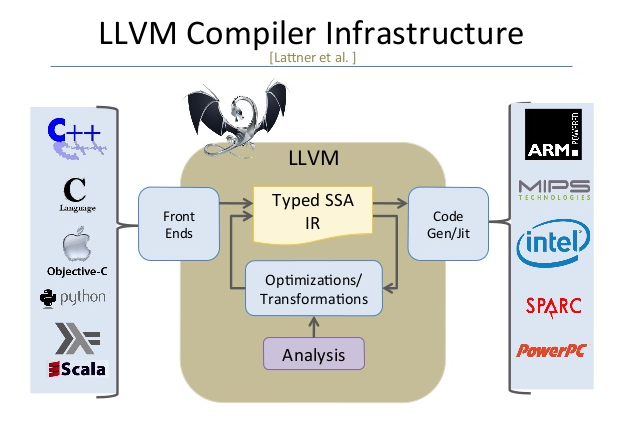
\includegraphics[width=.8\textwidth]{img/llvm.png}
    \caption{Illustration of the LLVM toolchain from Lattner et al.}
    \label{fig:llvm}
\end{figure}

\begin{listing}
    \begin{minted}{c}
#include <stdio.h>
int main()
{
    int i;
    i = 10;
    printf("Hello World! N = %d\n", i);
    return 0;
}
// gets compiled into...
    \end{minted}
    \begin{minted}{llvm}
@.str = private unnamed_addr constant 
    [21 x i8] c"Hello World! N = %d\0A\00", align 1
; Function Attrs: noinline nounwind optnone uwtable
define dso_local i32 @main() #0 {
  %1 = alloca i32, align 4
  %2 = alloca i32, align 4
  store i32 0, i32* %1, align 4
  store i32 10, i32* %2, align 4
  %3 = load i32, i32* %2, align 4
  %4 = call i32 (i8*, ...) @printf(i8* getelementptr inbounds 
        ([21 x i8], [21 x i8]* @.str, i64 0, i64 0), i32 %3)
  ret i32 0
}
declare dso_local i32 @printf(i8*, ...) #1
    \end{minted}
    \caption{A basic hello world program in human-readable LLVM-IR.}
    \label{lst:llvmir}
\end{listing}

\subsubsection{LLVM Instructions}
With the generated LLVM-IR we can now build a graph, by interpreting the individual LLVM instructions as constraints for a chosen pointer analysis.
The LLVM-IR uses static single assignment (SSA) form for variables meaning that each variable can only be assigned a single time in a specific control flow in the intermediate representation.
The use of SSA form is not directly relevant to Andersen style analyses but simplifies working with variables conceptually, since no variable can be reassigned at any point of the program.
At this point it is also important to differentiate between address-taken variables and top-level variables.
Top-level variables' values reside in registers and are conceptually ephemeral while address-taken variables are abstract memory objects which logically reside in memory. The specifics of memory locations and cpu registers are of cause hardware specific and depend on the target architecture that the llvm backend assembles the intermediate representation into.
The connection between address-taken and top-level variables in the LLVM-IR is established by the \verb|alloca| instruction which maps a top-level variable to a memory location represented by an address-taken variable.
Following is an interpretation of the LLVM instructions for Andersen's pointer analysis.

\paragraph{Load Instruction}
The LLVM \verb|alloca| instruction is used to allocate memory on the stack.
\begin{minted}{llvm}
    ; allocate a pointer to a 32 bit integer on the stack 
    ; and save a reference at ptr
    %ptr = alloca i32*, align 8
\end{minted}
The analog of the \verb|alloca| instruction in a pointer analysis is the address-of operation $x = \&a$, since the top-level variable $ptr$ points to the abstract memory location holding the actual value.
This might come as a surprise, since the implementation of $x = \&a$ in C does not result in an \verb|alloca| instruction. This often leads to confusion when interpreting points-to results that are built using the LLVM-IR.

\paragraph{Load Instruction}
The LLVM \verb|load| instruction loads the value on a top-level variable into a new variable. Compared to the C programming language this is comparable to dereferencing a pointer variable.
\begin{minted}{llvm}
    %ptr = alloca i32*, align 8
    ; load the pointer to the 32 bit integer from ptr into %var
    %var = load i32*, i32** %ptr, align 8
\end{minted}
When interpreting LLVM load instructions for a pointer analysis, we can treat it as the complex load constraint that is already defined for Andersen's analysis in \autoref{tab:ander}.
Again just like the alloca instruction we can not draw a direct comparison between the definition of the constraint $x = *y$ and the equivalent statement in the C language, since we are working with the LLVM-IR in SSA form.
The C equivalant would be the dereferencing of $*y$ alone. The assignment to x would require another store instruction.

\paragraph{Store Instruction}
The LLVM \verb|store| instruction stores a value into a variable. The variable might be a top-level or an abstract memory object represented by an address-taken variable.
\begin{minted}{llvm}
    %ptr = alloca i32*, align 8
    %var = load i32*, i32** %ptr, align 8
    ; store the literal value 10 into %var
    store i32 10, i32* %var, align 4
\end{minted}
The interpretation of the LLVM store instruction is similar to the load instruction. It can be interpreted as the complex store constraint defined as part of Andersen's analysis.

\paragraph{Getelementptr Instruction}
The LLVM \verb|getelementptr| or \verb|gep| instruction is used to get subelements from an aggregate data structure such as arrays or structs. When the gep instruction is invoked, it requires an index in order to perform the address calculation for the subelement. Getelementptr does not access memory, it only finds the correct address.
\begin{minted}{c}
    int arr[10];
    arr[5] = 10;
\end{minted}
\begin{minted}{llvm}
    ; create an integer array
    %arr = alloca [10 x i32], align 16
    ; get the address for the 5th element
    %idx = getelementptr inbounds [10 x i32], [10 x i32]* %arr, 
        i64 0, i64 5
    store i32 10, i32* %idx, align 4
\end{minted}
Since we intend to run a static analysis, we need to consider the properties of the index value passed into the getelementptr instruction.
Either the index is a constant value, and we can forward the gep instruction together with the constant index into the static analysis,
or the index is a variable that is subject to change during execution, and we need to assume that every possible value can be realized during execution, i.e. every offset for an aggregate data structure might be referenced by such a gep instruction and this information must be passed to the static analysis.
This behaviour is handled by differentiating between two types of gep constraints in the pointer analysis, normal- and variant-gep constraints. The former specifying a singular offset and the latter every possible offset for a given aggregate data type, since the value can not be statically determined.

\paragraph{Copy Instruction and equivalant Instructions}
Other than the complex store, load and the address-of constraints, the Andersen inclusion-based pointer analysis operates also on simple constraints, see line 2 in \autoref{tab:ander}. In terms of LLVM-IR instructions we are only interested in those instructions that manipulate pointers. In the LLVM-IR specification lots of instructions can result in values being moved, including pointers. Therefore we group those instructions that can move values between symbols under the simple inclusion-based constraint.
The following instructions are interpreted as simple constraints:
\begin{itemize}
    \item \verb|Phi| instructions are part of the LLVM-IR to correctly resolve control flow. Depending on the conditional branch a new SSA variable is introduced that holds the resulting value from the branch.
          Since we are implementing a flow-insensitive pointer analysis we do not differentiate between constrol flows and simply interpret each phi instruction as a simple constraint connecting the conditional values to the resulting phi variable.
    \item \verb|Select| instructions serve a similar purpose as phi instructions. Here a value is selected conditionally without creating branches. As such we interpret the select instruction as a simple constraint.
    \item \verb|Call| instructions represent a function call. If the function call contains arguments the caller arguments and callee parameters need to be interpreted as a simple constraint. Beyond this, nothing is done to analyze the context of the function call, since we are performing a context-insensitive pointer analysis.
    \item Like the call instructions, \verb|Ret| instructions are simply interpreted as simple constraints so the returned function value is included in the pointer analysis.
    \item \verb|ThreadFork| \verb|ThreadJoin| are not LLVM-IR instruction. But just like the call and ret instructions, these must be interpreted as function calls with simple constraints in the context of pointer analysis.
    \item Lastly there are various instructions that are straightforward to interpret as simple constraints, including \verb|bitcast|, \verb|ptrtoint| and \verb|freeze| instructions. Furthermore variable argument values and external library call parameters need to be handled like regular call instructions.
\end{itemize}

Now with alloca, load and store instructions introduced, we can analyze a basic example during pointer analysis.
We are going to observe a simple c program:
\begin{minted}{c}
    int *p, x, *q;
    p = &x;
    q = p;
\end{minted}
Which will compile into the following LLVM-IR:
\begin{minted}{llvm}
    %1 = alloca i32*, align 8
    %2 = alloca i32, align 4
    %3 = alloca i32*, align 8
    store i32* %2, i32** %1, align 8
    %4 = load i32*, i32** %1, align 8
    store i32* %4, i32** %3, align 8
\end{minted}
An example for applying the constraint rules according to the Andersen algorithm in \autoref{tab:ander} can be observed in \autoref{tab:applyander}.
The edge labels of the constraint graph are \verb|p|, \verb|s|, \verb|l|, \verb|c| corresponding to points-to (inverse alloca), store, load and copy constraints.
Furthermore the copy edges are immediately converted into point-to edges in order to simplify the constraint graph.

\begin{table}[H]
    \caption{Applying Andersen Constraints}
    \centering
    \label{tab:applyander}
    \begin{tabular}{p{0.5\textwidth} c c}
        \toprule
        Code Snippet to analyze / comment                & Constraint Graph                                                                          \\
        \midrule
        \begin{minipage}[t]{0.5\textwidth}
            \begin{minted}{llvm}
%1 = alloca i32*, align 8
%2 = alloca i32, align 4
%3 = alloca i32*, align 8
            \end{minted}
        \end{minipage}            & 
        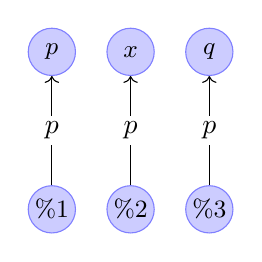
\begin{tikzpicture}[baseline=0]
            \tikzstyle{node}=[circle, draw=blue!50, fill=blue!20, inner sep=1pt, minimum size=6mm]
            \tikzstyle{linenode}=[pos=0.5,fill=white,inner sep=2pt,outer sep=2pt]
            \node[node] (A) at (0,-2) {\small$\%1$};
            \node[node] (B) at (1,-2) {\small$\%2$};
            \node[node] (C) at (2,-2) {\small$\%3$};
            \node[node] (Ap) at (0,0) {\small$p$};
            \node[node] (Bp) at (1,0) {\small$x$};
            \node[node] (Cp) at (2,0) {\small$q$};
            \path [->] (A) edge[] node[linenode] {$p$} (Ap);
            \path [->] (B) edge[] node[linenode] {$p$} (Bp);
            \path [->] (C) edge[] node[linenode] {$p$} (Cp);
        \end{tikzpicture}                                                        \\
        \midrule
        \begin{minipage}[t]{0.5\textwidth}
            \begin{minted}{llvm}
store i32* %2, i32** %1, align 8
            \end{minted}
        \end{minipage} & 
        \begin{tikzpicture}[baseline=0]
            \tikzstyle{node}=[circle, draw=blue!50, fill=blue!20, inner sep=1pt, minimum size=6mm]
            \tikzstyle{linenode}=[pos=0.5,fill=white,inner sep=2pt,outer sep=2pt]
            \node[node] (A) at (0,-2) {\small$\%1$};
            \node[node] (B) at (2,-2) {\small$\%2$};
            \node[node] (C) at (3,-2) {\small$\%3$};
            \node[node] (Ap) at (0,0) {\small$p$};
            \node[node] (Bp) at (2,0) {\small$x$};
            \node[node] (Cp) at (3,0) {\small$q$};
            \path [->] (A) edge[] node[linenode] {$p$} (Ap);
            \path [->] (B) edge[] node[linenode] {$p$} (Bp);
            \path [->] (C) edge[] node[linenode] {$p$} (Cp);
            \path [->] (B) edge[] node[linenode] {$s$} (A);
            \path [->] (A) edge[] node[linenode] {$l$} (D);
        \end{tikzpicture} \\
        \midrule
        \begin{minipage}[t]{0.5\textwidth}
            \begin{minted}{llvm}
%5 = load i32, i32* %4, align 4
store i32 %5, i32* %3, align 4
            \end{minted}
        \end{minipage} & 
        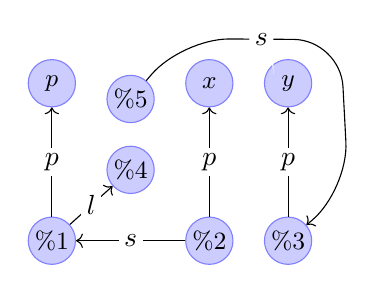
\begin{tikzpicture}[baseline=0]
            \tikzstyle{node}=[circle, draw=blue!50, fill=blue!20, inner sep=1pt, minimum size=6mm]
            \tikzstyle{linenode}=[pos=0.5,fill=white,inner sep=2pt,outer sep=2pt]
            \node[node] (A) at (0,-2) {\small$\%1$};
            \node[node] (B) at (2,-2) {\small$\%2$};
            \node[node] (C) at (3,-2) {\small$\%3$};
            \node[node] (Ap) at (0,0) {\small$p$};
            \node[node] (Bp) at (2,0) {\small$x$};
            \node[node] (Cp) at (3,0) {\small$y$};
            \node[node] (D) at (1,-1.1) {\small$\%4$};
            \node[node] (E) at (1,-0.2) {\small$\%5$};
            \path [->] (A) edge[] node[linenode] {$p$} (Ap);
            \path [->] (B) edge[] node[linenode] {$p$} (Bp);
            \path [->] (C) edge[] node[linenode] {$p$} (Cp);
            \path [->] (B) edge[] node[linenode] {$s$} (A);
            \path [->] (A) edge[] node[linenode] {$l$} (D);
            \draw[->, rounded corners=6mm] (E) -- ($(E.60) + (0.5,0.5)$) -- ($(Cp.30) + (0.4,0.4)$) node[linenode]{$s$} -- ($(C.30) + (0.5,0.5)$) -- (C);
        \end{tikzpicture} \\
        \bottomrule
    \end{tabular}
\end{table}

go through instrs, and how they are relevant to pta, explain constraints \cite{lin2015alias}
\section{Related Work}
\subsection{Context Free Languages}
first general idea: \cite{reps1998program} first idea of gemm for cflpq \cite{azimov2018context} kronecker product idea \cite{orachev2020context} evaluation \cite{mishin2019evaluation} spbla library \cite{orachev2021spbla}, current draft [Taming Transitive Redundancy for Context-Free Language Reachability] fron SVF, parallel pta via cfl \cite{su2014parallel}
\subsection{Sequential Analyses}
\subsubsection{SVF}
svf idea, built on top of llvm, \cite{sui2016svf}, briefly explain all subcomponents i.e. memleak detection: \cite{sui2014detecting} demand driven VF: \cite{sui2018value} new alternative, faster, better results than svf \cite{shi2018pinpoint}
\subsection{GPU Accelerated Analyses}
\subsubsection{Graspan}
original idea \cite{zheng2008demand} big data approach on cpu \cite{wang2017graspan} and gpu \cite{zuo2021systemizing} alternative impl \cite{gu2020towards} based on \cite{mendez2012gpu} and \cite{mendez2010parallel}
\section{Motivation}
general alias analysis is undecidable
This thesis aims to explore the possibilities of parallelizing the Andersen style inclusion based whole program pointer analysis. The goal is to improve static pointer analysis performance by using massively parallel GPUs.
With the general trend of more complex software systems in software development, developers also require static analysis tools that are able to perform scalable analyses on entire codebases.
Unfortunately general pointer analysis is undecidable problem, which is a problem that prevents maximally precise pointer analysis from being a possibility.
For this reason a balance must be found between performance and precision when analyzing code.
Historically most pointer analysis solutions have been implemented as single threaded applications. By using GPGPUs the proposed library from this thesis aims to improve performance when analyzing entire programs by distributing the work accross the many streaming processors modern GPGPUs possess. The proposed performance improvement also does not decrease the analysis precision.
\subsection{Static Analysis in Software Development}
finding bugs is becoming harder

inter procedural analysis scalability; create a single machine implementation that used parallel hardware and integrates into SVF

\begin{figure}
    \centering
    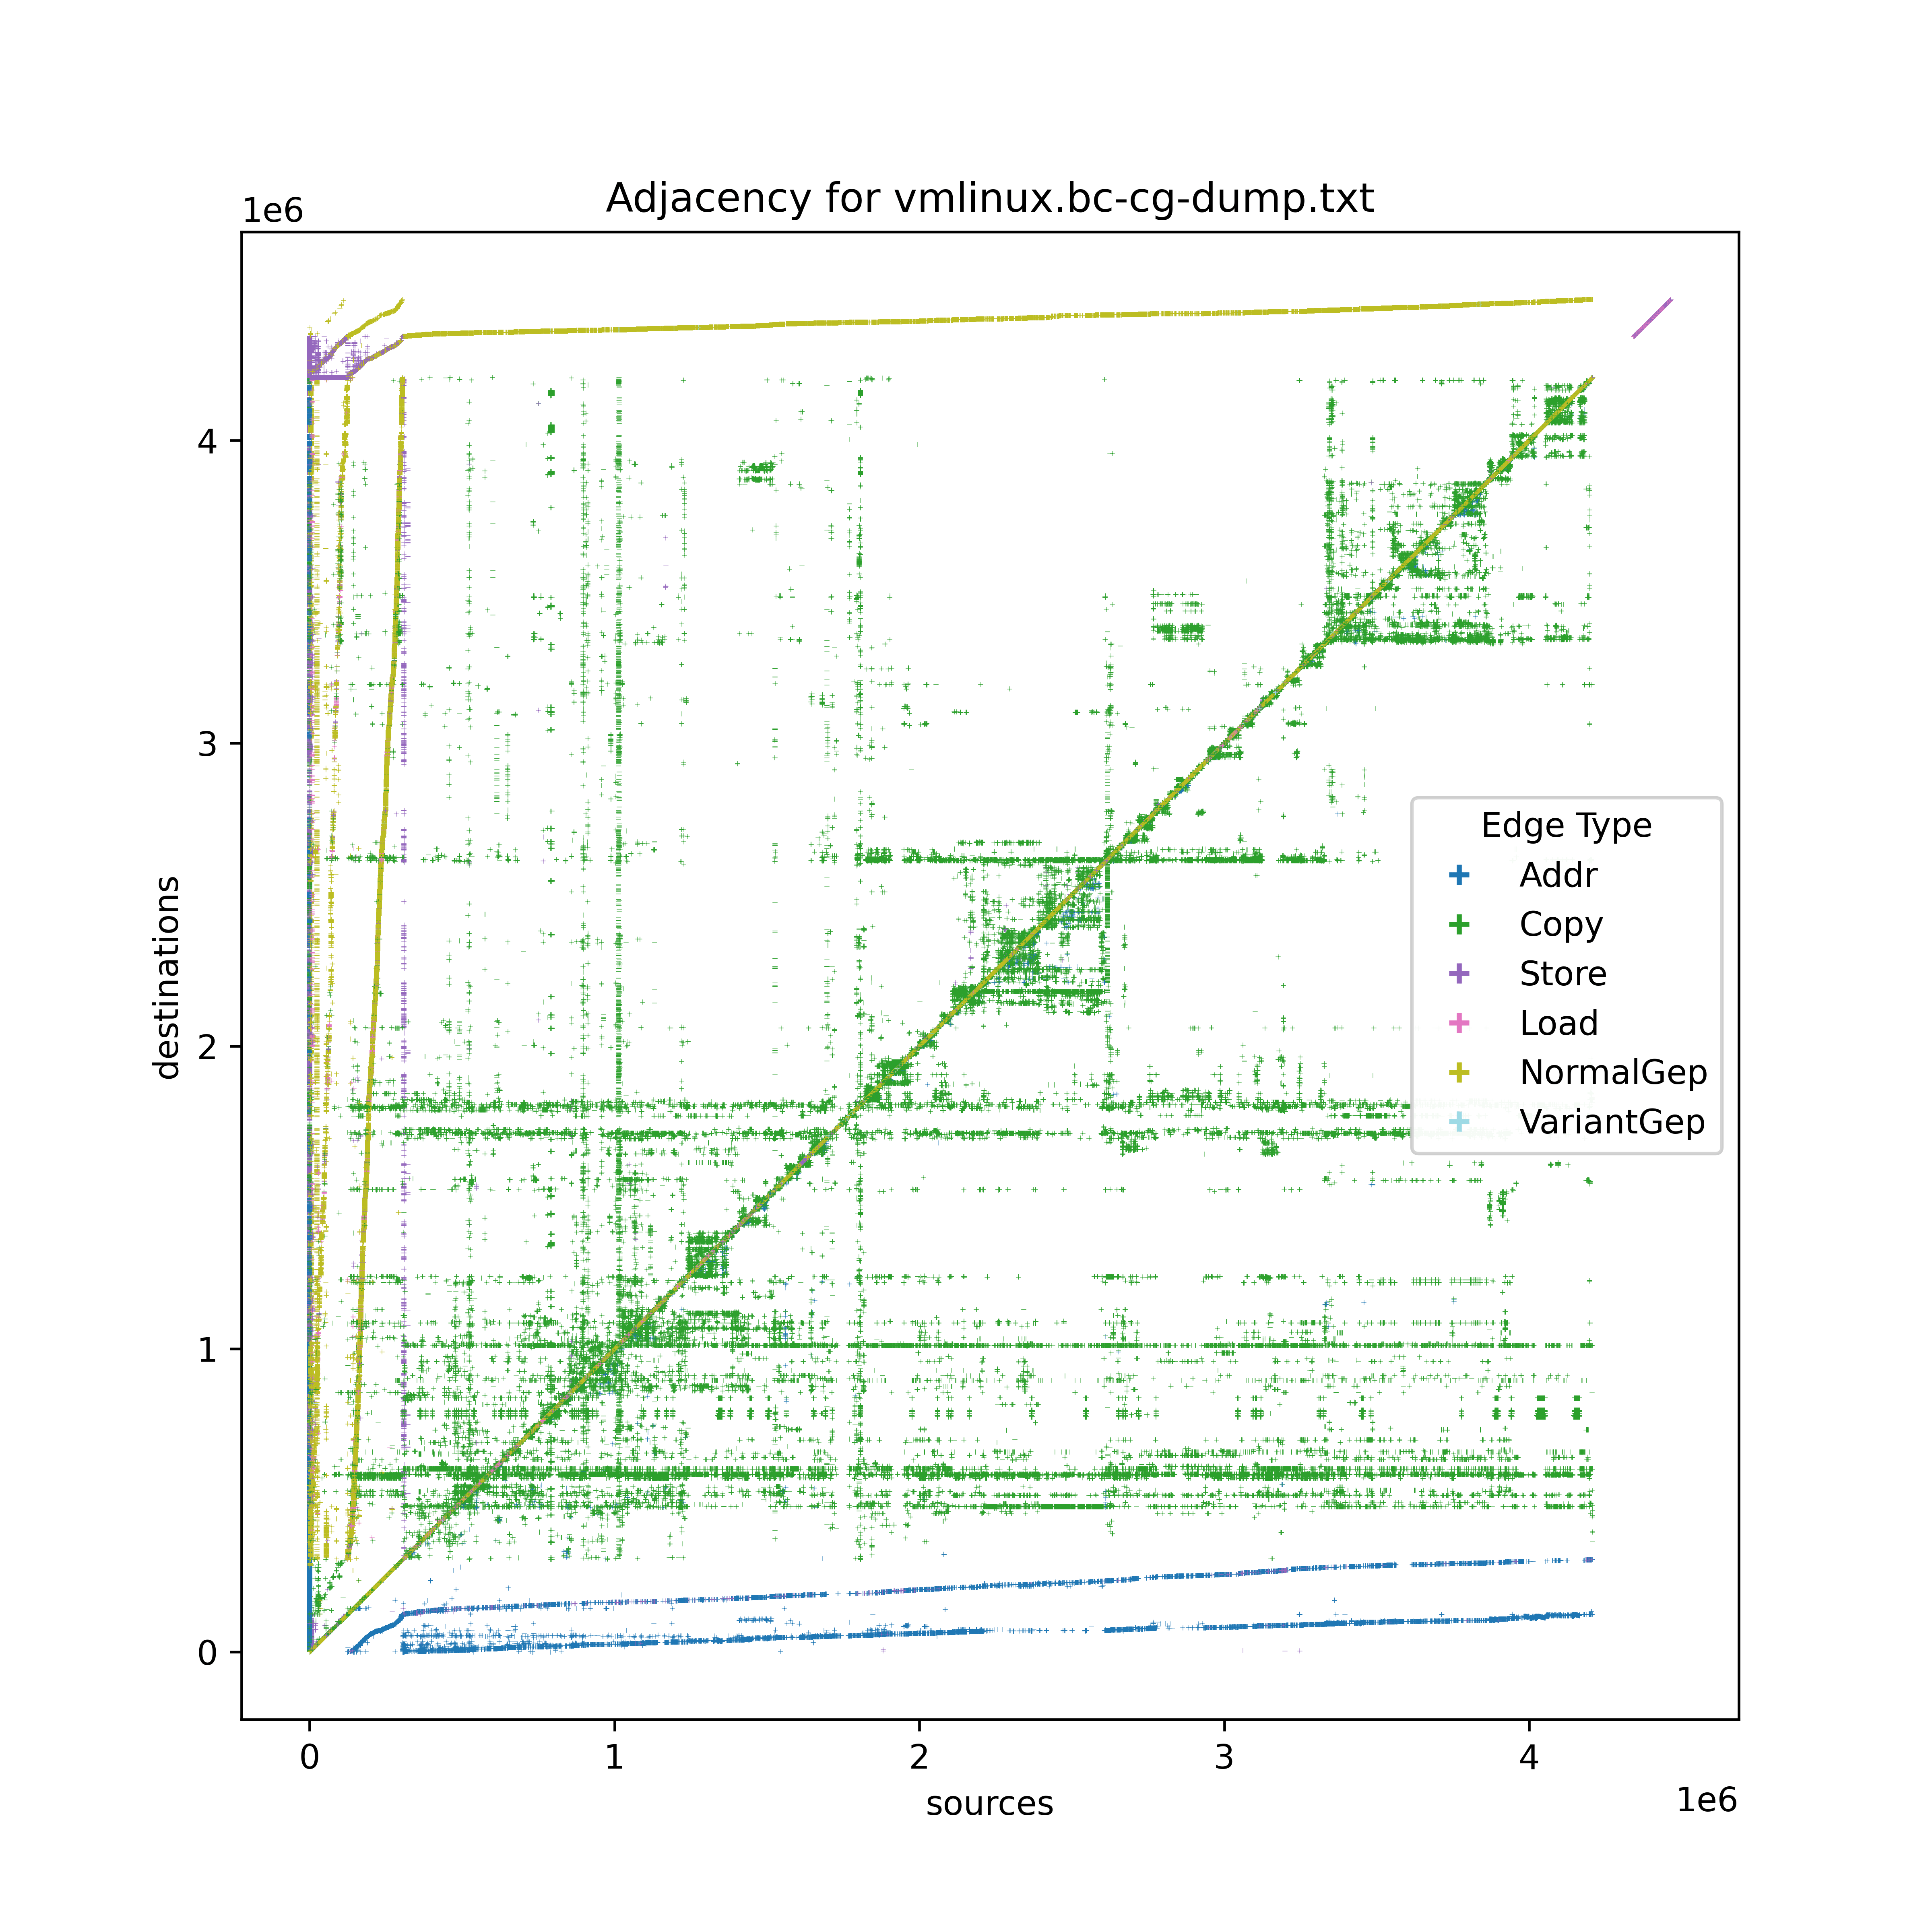
\includegraphics[width=1.\textwidth]{img/linux-consg-min.png}
    \caption{Adjacency Plot for the Constraint Graph of the Linux Kernel}
    \label{fig:linux-consg}
\end{figure}


\begin{table}
    \begin{center}
        \caption{More rows.}
        \label{tab:table1}
        \begin{tabular}{l|S|r}
            \textbf{Value 1} & \textbf{Value 2} & \textbf{Value 3} \\
            $\alpha$         & $\beta$          & $\gamma$         \\
            \hline
            1                & 1110.1           & a                \\
            2                & 10.1             & b                \\
            3                & 23.113231        & c                \\
            4                & 25.113231        & d                \\ % <-- added row here
        \end{tabular}
    \end{center}
\end{table}

\chapter{PTAGPU} \label{chap:main}
This thesis presents a software library named PTAGPU, the name is derived from pointer analysis (PTA) and graphics processing unit (GPU).
As the name suggests the core idea is to use GPUs for the purpose of performing a pointer analysis.
The library PTAGPU was developed as a whole program analysis module inside the SVF framework which is in turn built on top of the LLVM compiler system.
\section{Integrating PTAGPU into SVF}\label{sec:integsvf}
As described in \autoref{sec:svf} the SVF framework is capable of processing the LLVM-IR of a compiled program and capture the individual LLVM-IR instructions in a program assignment graph.
When SVF is launched for a whole program analysis, the program assignment graph is further processed into a constraint graph that holds holds all relevant constraints for an initial pointer analysis, see \autoref{tab:ander}.
At this point the constraint graph is passed into a class that inherits from the PointerAnalysis class, see \autoref{fig:pta-svf} for an overview of the pointer analysis class hierarchy in SVF.
Since our goal is to implement a custom pointer analysis, we can inject out own implementation at this stage as a PointerAnalysis subclass.
Specifically we inherit from the Andersen class which is itself a subclass of the PointerAnalysis class that implements the Andersen inclusion-based pointer analysis algorithm in SVF.
By extensive use of runtime polymorphism most of SVF is implemented via virtual member functions - a construct specific to c++ - allowing for function overriding in subclasses. This makes implementing a custom pointer analysis easy as we can reuse most of the initialization steps and program assignment graph processing from the superclasses. Part of the processing is an initial topological sorting and the previously mentioned interpretation into a constraint graph.
As a result we end up with a constraint graph and all strongly connected components of said graph when we initialize our PTAGPU class that inherits from the Andersen class.
The in-memory representation of constraint graphs or generic graphs in SVF is more akin to a linked list data structure where each node carries references to all outgoing and incoming edges and those edges carry references to source and destination nodes as well as auxiliary information, which is an ideal memory model for iterative algorithms such as the default Andersen algorithm where the algorithm works from one node to the next.
Unfortunately this memory model is not ideal for parallel processing.
For this reason we initially reinterpret the constraint graph into a more fitting data structure.
While iterating through the entire constraint graph, we differentiate by edge types and collect all $(src,dst)$ edge pairs in standard library vectors.
If we refer back to the design principles of SVF in \autoref{sec:svf}, where pointer analyses were conceptually split into three components, the Rules, the Graph and the Solver, we effectively implement our own Graph component by using a different linear memory representation for the constraint graph. 
The underlying goal of putting the constraint graph into a linear in-memory data structure is to allow us to more easily copy the memory region containing the relevant information into GPU device memory, which is where our pointer analysis will operate on the data.
Similarly to the Graph component we also modify the Solver and Rule components in the custom analysis implementation.
The details of the implementation will be described in detail in \autoref{sec:design}.

\section{Goal of the Algorithm}
Our goal is to use the provided program assigment graph from SVF and the derived constraint graph to compute a points-to set for each pointer variable in the program.
Overall our algorithm is supposed to serve as an initial pointer analysis pass in the SVF framework. Together with the pointer information we can then proceed to build an over-approximated call graph.
One might assume that no pointer information is needed for SVF to build a call graph for the program. Unfortunately indirect function invocations, where function are accessed by pointer dereferencing itself, requires us to build pointer information in order to create an over-approximated sound call graph. The over-approximate nature stems from the imprecision of Andersen's analysis. This limitation always remains, no matter the algorithm, since pointer analyses are fundamentally undecidable as was mentioned in \autoref{sec:pta}.
It is important to consider that the initial pointer analysis does not directly produce any valuable information in terms of static analysis purposes. Instead we use the pointer information produced by the initial analysis for the call graph which is then used to refine the analysis result by applying a more precise flow- and/or context-sensitive analysis that produces the relevant results, which can then be used to derive value flow information that can directly be used for actual analysis purposes.
Since we are applying a more precise pointer analysis at a later stage anyways one might argue that it would be wise to start off with such an analysis. For small programs this is a viable strategy, unfortunately these more precise analyses are currently not scalable for a whole program analysis and are only applied on-demand \cite{sui2016svf}. This is also one of the motivations for trying to accelerate the initial Anderen analysis specifically since it is performed on the entire program and thus can in theory profit from the paralellism of GPUs.

\section{Design of the Algorithm}\label{sec:design}
The PTAGPU library uses CUDA\footnote{\url{https://developer.nvidia.com/cuda-toolkit}}, an application programming interface language from NVIDIA, to program GPUs in C++.
CUDA accomodates developers with a collection of abstractions that simplify operations with GPU compute and memory. NVIDIA also provides a standalone library for common parallel oeprations such as sorting and transformations named Thrust\footnote{\url{https://docs.nvidia.com/cuda/thrust/index.html}} which is also employed by PTAGPU for common sorting and deduplication operations.
In principle all calculations that are executed with a GPU are denoted as kernels in CUDA. While GPU kernels and CPU code can be shared, CUDA provides some intrinsic operations that can only function when executed on a GPU.
Likewise all CPU operations that rely on external libraries or non standard-library code are not supported in GPU kernels.

\subsection{CUDA Architecture}
The CUDA programming model revolves around blocks of threads. Each block of a kernel executes the same code with the same number of threads.
Thread blocks are further divided into Warps, which are a collection of 32 threads each. This type of parallel processing is called SIMT, for single instruction, multiple threads.
In reality a Warp is more analogous to a single vectorized operation that executes 32 units of work or lanes at once than a collection of individual threads, although each thread in a Warp has its own instruction address counter. Having instruction address counters per thread allows independent branching, resulting in thread divergence. The divergence is implemented by executing each conditional branch sequentially for all threads in a Warp and disabling the threads that do not execute the specific branch.
This way each thread in a Warp always executes the same instruction if active. Since branches are not executed in parallel, thread divergence is discouraged if possible for performance reasons.
These specifications of Warps are uniform in all CUDA hardware and resemble a single group of work that can be scheduled on the device specific number of multiprocessors.
To more easily differentiate between different generations of hardware, the CUDA programming model is segmented into tiers of compute capabilities, where newer hardware with newer capabilities receives a higher compute capability.
Each CUDA capable device has a number of streaming multiprocessors, in short SMs, which themselves have a certain amount of L1 shared memory and number of registers per core among other resources. 
While this is similar to how CPU cores operate, GPU programming uses a flat memory hierarchy with less reliance on caching and more on raw memory bandwidth. For this reason each core in an SM has a relatively large register file so that a single CUDA thread commonly uses hundreds of registers.
The entire work that is to be performed by a single kernel is called a grid, which is divided evenly into blocks, which are divided into Warps. Both the grid and each block can be indexed in up to three dimensions, which is useful for working with shader, global illumination rendering and less useful for static analyses.
To start a computation, a collection of thread blocks are assigned to the available SMs of a GPU. Depending on the hardware and compute capability, a single SM can execute multiple Warps from the assigned thread blocks in parallel as long as enough resources are available in the SM.
\begin{figure}
    \centering
    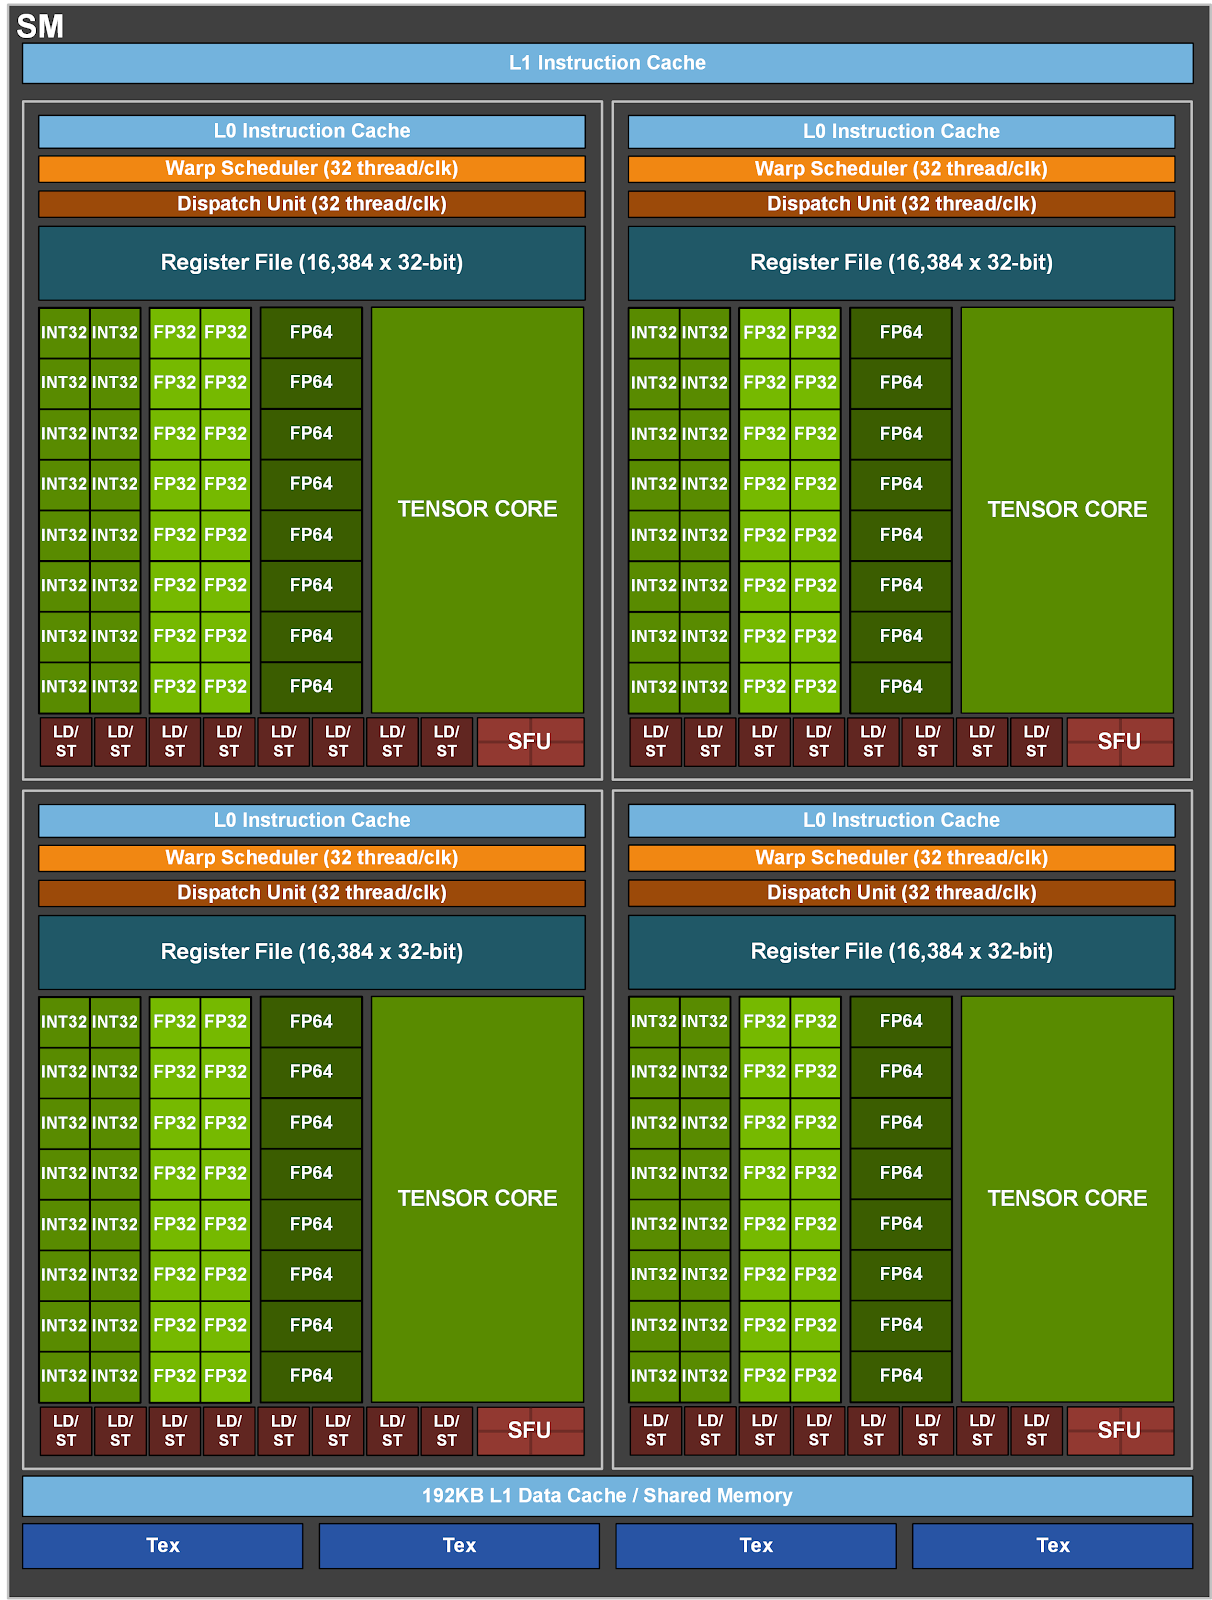
\includegraphics[width=.7\textwidth]{img/a100.png}
    \caption[Diagram of a single A100 SM]{A single SM of an A100 GPU.\\Taken from an NVIDIA Blog Post\footnotemark}
    \label{fig:cuda-sm}
\end{figure}
\footnotetext{\url{https://developer.nvidia.com/blog/nvidia-ampere-architecture-in-depth/}}
The execution order of individual Warps is handled by a Warp scheduler, that decides what Warps get executed at what time.
The purpose of overprovisioning SMs with more blocks/Warps than they can concurrently execute is that when a single Warp executes a memory read/write operation other Warps can execute while the device is busy fetching the data.
Key specification for each SM of a certain compute capability are the following:
\begin{itemize}
    \item Memory Bandwith per SM
    \item Total shared memory per SM
    \item Max number of threads per SM
    \item Max number of blocks per SM
    \item Total number of registers of all cores in SM
\end{itemize}

\subsubsection{Occupancy}
Since each SM has multiple limited resources that can be controlled by the developer, namely register count, shared memory and thread count, a kernel has to be designed with these limitations in mind such that a maximally concurrent execution is possible.
Given a device with compute capability 8.0 and a kernel that requires 256 registers per thread while also running 256 threads per block, we would essentially limit our execution to a single block per SM, since a device with compute capability 8.0 has 64K registers per SM.
This might be disadvantageous, since the SM is in theory capable of working on up to 1024 threads.
We might profit from reducing the amount of registers used per thread and thus increasing the occupancy on our GPU.
Counterintuitively high occupancy does not always lead to better performance. Some programs disproportionally profit from the use of a single resource.
For example compute intensive kernels require more registers per thread than kernels that are heavily reliant on memory operations. Increasing the use of shared memory does not always lead to a performance improvement and decreasing the number of required registers is not always possible.
\subsubsection{Memory Accesses in CUDA}
While modern GPUs can in theory perform multiple TFLOPS of calculations per second, effectively all calculations are limited by memory bandwidth.
Consequently, how we access the GPU memory is very important for the overall performance of our analysis. Specifically coalesced memory accesses of individual Warps where consecutive threads access consecutive memory addresses are important so the memory read operation can be performed within a single transaction and not multiple strided reads.
\begin{figure}
    \centering
    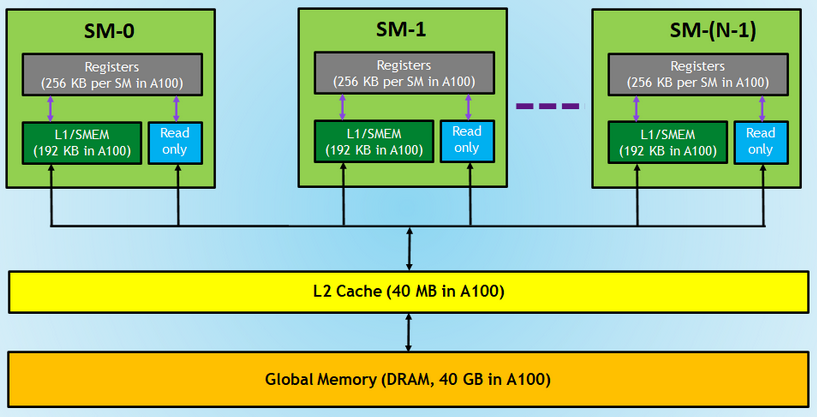
\includegraphics[width=.7\textwidth]{img/cuda.png}
    \caption[Diagram of the CUDA memory architecture for an A100]{Diagram of the CUDA memory architecture for an A100 GPU.\\Taken from \cite{cudarefresher}.}
    \label{fig:cuda-arch}
\end{figure}
The GPU memory controller on modern graphics cards can typically execute memory read or write operations in granularities of 32 bytes up to 128 bytes in total.
As a result it is for example more efficient to load a single byte of memory per thread in a Warp, compared to loading 8 bytes per thread, since we would exceed the maximum of 128 bytes per memory transaction and require multiple memory accesses.
In terms of time needed per instruction, global memory operations are typically two orders of magnitude slower compared to operations on SM registers or shared memory in L1 cache. For this reason CUDA programs can perform exponentially worse if memory accesses are random or strided inefficiently instead of coalesced.

\subsubsection{Unified Memory}
When CUDA code is executed on a 64-bit host system, the developer can use a single memory address space for host and device memory.
Using this unified memory address space allows memory access from both CPU and GPU in the same address space without explicit memory copy operations.
The memory in question is moved implicitly to the device that performs the read operation. The CUDA API also allows the developer to assign preferred residency for specific memory regions, as well as prefetching memory asynchronously for a device. When prefetching is properly employed, unified memory achieves the same performance as dedicated device memory \cite{cudaunifiedmem}.
The major advantage of unified memory is the fact that the memory allocation size is only limited by system memory, not device memory.
This allows a CUDA program to potentially hold vastly more data in memory than would be possible with only GPU memory, while also moving the needed memory regions without much involvement of the developer.
Crucially this keeps large data structures intact without splitting and partitioning them for incremental loading into GPU memory.
This mirrors some of the core ideas of Graspan \autoref{sec:graspan} where parts of the graph are written to disk to conserve memory usage.
Since many high performance computing environments have vastly more main memory available than individual GPUs have device memory, this enables us to expand the scope of our analysis without requiring specialized GPU hardware.

\subsubsection{CUDA Streams}
GPUs are massively parallel. Oftentimes developers do want to perform multiple computations encapsulated in kernels in parallel.
These computations require memory operations before and after to load and store the data to operate on.
Since most GPUs allow for concurrent memory and compute operations it is desirable to be able to efficiently schedule concurrent operations such that while one kernel executes, another performs memory operations.
Because kernels are launched asynchronously, we can utilize CUDA streams to string together multiple compute and memory operations so they are executed in order without interfering with other streams.
The GPU is then able to efficiently schedule multiple streams in order to maximize GPU utilization, see  \autoref{fig:cuda-stream} for an illustration.
By default all cuda operations are executed on the default stream and thus memory operations block each other.
Streams have to be created by the developer and are represented by structs in the program. These elements are then passed as arguments to the CUDA api function calls.

\begin{figure}
    \centering
    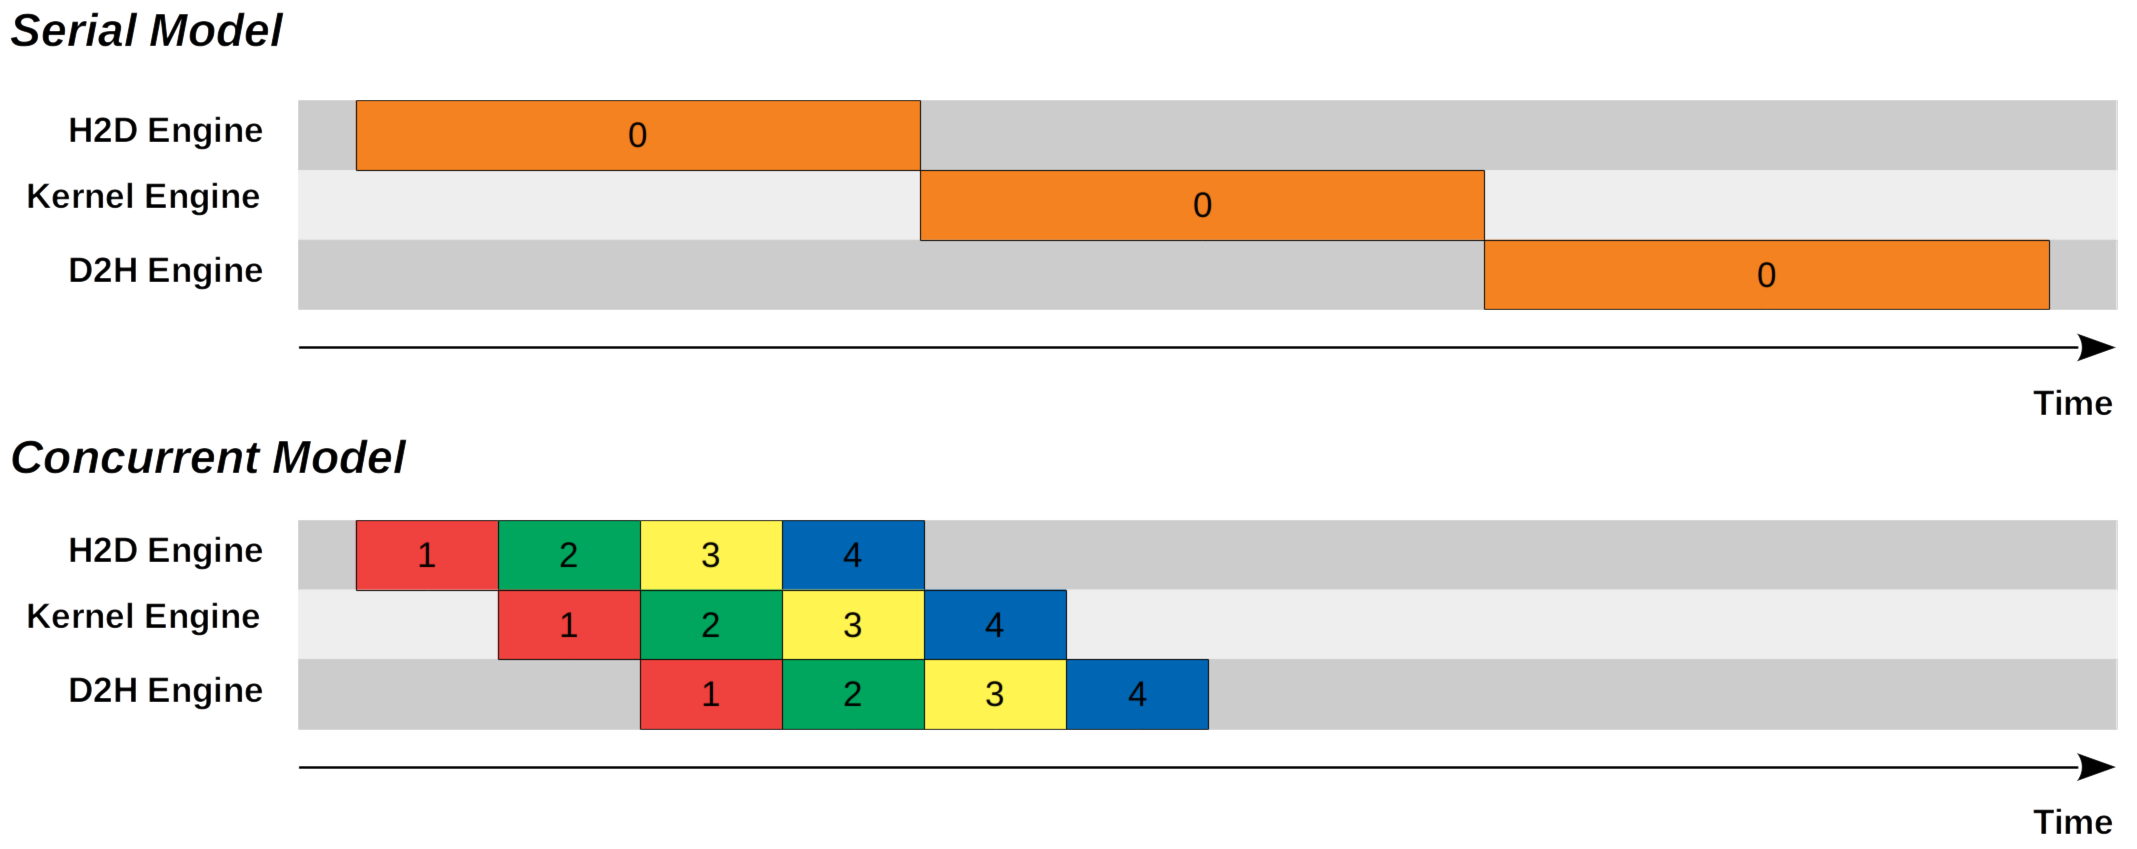
\includegraphics[width=1.\textwidth]{img/cuda-stream.png}
    \caption[CUDA strean illustration]{CUDA Stream: Serial Model vs Concurrent Model by Lei Mao łicensed under \href{https://creativecommons.org/licenses/by/4.0/}{CC BY 4.0}; an illustration for the advantages of the CUDA stream api.}
    \label{fig:cuda-stream}
\end{figure}

\subsection{Initialization of CUDA code}\label{sec:init}
As soon as the constraint graph is handed over to the CUDA section of the code some global state is initialized with the information from the constraint graph.
This includes various counter variables for the number of nodes in the graph, as well as the initial unified memory allocations.
When the counter for the number of nodes is first initialized the node count is read from the constraint graph and increased by 20 percent to reserve headroom for new nodes that might be added to the constraint graph during the execution of the algorithm.
This ensures that each node has a well defined place in memory that can not be overwritten by subsequent nodes.
In the current implementation, the algorithm allocates a fixed amount of unified memory accessible from the CPU and GPU. While this requires overprovisioning of memory for a given analysis without knowing the exact amount needed for the pointer analysis, dynamic allocation proves to be very challenging as it is difficult to deduce the exact required amount of GPU memory from a given constraint graph for a pointer analysis.
Furthermore the allocated unified memory is further split into partitions of fixed size for the individual relations of the Andersen analysis.
This includes three memory regions for pointer relations, one for copy relations and two regions for load and store relations between nodes.
See the following diagram for the memory layout of an example allocation of 32 GiB of unified memory.
\begin{center}
    \begin{bytefield}{32}
        \begin{rightwordgroup}{includes all pointer relations\\that have been computed\\at any stage}
            \memsection{ffff ffff}{a000 0000}{12}{pointer constraints}
        \end{rightwordgroup}\\
        \begin{rightwordgroup}{these memory regions are used\\to compute the delta updates\\for the pointer relations}
            \memsection{9fff ffff}{6000 0000}{8}{current pointer constraints}\\
            \memsection{5fff ffff}{2000 0000}{8}{next pointer constraints}
        \end{rightwordgroup}\\
        \begin{rightwordgroup}{static memory\\does not change once written}
            \memsection{1fff ffff}{1000 0000}{2}{load constraints}\\
            \memsection{0fff ffff}{0000 0000}{2}{store constraints}
        \end{rightwordgroup}\\
    \end{bytefield}
\end{center}
Since a pointer analysis in general does not create new load or store relations in the constraint graph, these memory regions do not increase in size after initialization.
Notably the pointer relations are split into three separate memory regions. This is needed for diffpoints calculations. This specific optimization was inspired by \cite{mendez2010parallel} among other works and will be explained in detail in \autoref{sec:diffpts}.
After memory allocation is completed, CUDA streams are initialized for concurrent write operations into each memory region, as well as one stream for each of the available devices to enable computation on multiple GPUs in parallel.
Finally the entire allocation of unified memory is set to ones by \verb|cudaMemset|. This ensures that the memory is not in an undefined state. Furthermore we can utilize this when reading from memory, since a memory region with all bits set to one represents unused space.

% This state is needed for the 

% initializing cuda V var, overhead for new nodes

% subsec unified memory explain

% subsec explain sparse bv layout

% go through idea of inv edges for concurrent rewriting

% based on \cite{mendez2010parallel} and \cite{mendez2012gpu}



% \begin{center}
%     \begin{bytefield}{32}
%         \bitheader{0-31} \\
%         \bitbox{4}{Four} & \bitbox{8}{Eight} &
%         \bitbox{16}{Sixteen} & \bitbox{4}{Four}
%     \end{bytefield}
% \end{center}
% \blindtext[1]
% \begin{center}
%     \definecolor{lightcyan}{rgb}{0.84,1,1}
%     \definecolor{lightgreen}{rgb}{0.64,1,0.71}
%     \definecolor{lightred}{rgb}{1,0.7,0.71}
%     \begin{bytefield}[bitheight=\widthof{~Base~},
%             boxformatting={\centering\small},rightcurly=., rightcurlyspace=0pt]{32}
%         % \bitlabel{29}{Data} & \bitlabel{1}{Base} & \bitlabel{2}{Next} \\
%         \bitheader{0,28,29,30,31} \\
%         \begin{rightwordgroup}{
%                 \begin{tikzpicture}
%                     \tikzstyle{node}=[circle, draw=blue!50, fill=blue!20, inner sep=1pt, minimum size=6mm]
%                     \tikzstyle{linenode}=[pos=0.5,fill=white,inner sep=2pt,outer sep=2pt]
%                     \node[node] (A) at (0,0) {\small$\%1$};
%                     \node[node] (B) at (2,0) {\small$\%2$};
%                     \path [->] (A) edge[bend left] node[linenode] {$p$} (B);
%                 \end{tikzpicture}
%             }
%             \bitbox{29}[bgcolor=lightred]{Data} &
%             \bitbox{1}[bgcolor=lightcyan]{\rotatebox{90}{Base}} &
%             \bitbox{2}[bgcolor=lightgreen]{\rotatebox{90}{Next}}
%         \end{rightwordgroup}
%     \end{bytefield}
% \end{center}

\subsection{Sparse Bitvectors}
At the core of PTAGPU all edges of the constraint graph are stored in sparse bitvectors.
Sparse bitvectors are a data structure that can be used for storing binary values, such as adjacency information of a graph. Sparse bitvectors are especially suited to represent edges of very sparse graphs and allow for dynamic addition of new edges and nodes, something other sparse graph representation such as the compressed sparse row format do not facilitate. Since the constraint graph of pointer analysis problems is typically very sparse \cite{mendez2012gpu}, sparse bitvectors are an ideal data structure for pointer analysis on the GPU. Find the adjacency plot for the constraint graph of the linux kernel in \autoref{fig:linux-consg} as well as on overview for select open source programs and their constraint graph densities in \autoref{tab:benchmarkprograms}.
Individual bitvectors contain three separate component, a base value, a set of bits and a next pointer.
For the bitvectors to efficiently work, the entire codomain of the directed edge relation of a graph is split into evenly sized partitions.
The edges of each partition, if it contains edges, are then stored in the bits of a bitvector. If we omit empty partitions of the edge codomain, we create a set of sparse bitvectors.
The base value of each sparse bitvector represent the current offset for all bits in the bitvector.
Similar to linked lists, sparse bitvectors reference the next sparse bitvector in a field. This allows iteration through adjacent outgoing edges for a given node by working through the next bitvectors until there is no next bitvector defined.
The head bitvector for each node is stored in a pre defined memory location, which is directly derivable from the node index.
The exact position for each node in each memory partition can be calculated by multiplying the node index with the width of a sparse bitvector. This offset is then added to the overall offset of the memory partition to find the head bitvector for a specific edge type, see \autoref{lst:getindex} for the implementation in PTAGPU.
\begin{listing}
    \begin{minted}{c++}
// src it the node for which we want to find the head bitvector
// rel is the andersen relation for which we want to find the outgoing edges
__host__ __device__ index_t getIndex(uint src, uint rel)
{
    switch (rel)
    {
    case PTS:
        return OFFSET_PTS + (ELEMENT_WIDTH * src);
    case PTS_CURR:
        return OFFSET_PTS_CURR + (ELEMENT_WIDTH * src);
    case PTS_NEXT:
        return OFFSET_PTS_NEXT + (ELEMENT_WIDTH * src);
    case COPY:
        return OFFSET_COPY + (ELEMENT_WIDTH * src);
    case LOAD:
        return OFFSET_LOAD + (ELEMENT_WIDTH * src);
    case STORE:
        return OFFSET_STORE + (ELEMENT_WIDTH * src);
    }
    return src * ELEMENT_WIDTH;
}
    \end{minted}
    \caption{Calculating the correct index of a node's head bitvector in unified memory.}
    \label{lst:getindex}
\end{listing}
Following, each unit in the sparse bitvector linked list will be called an element as is conventional for linked lists.
When deciding on the memory characteristics of the individual elements, the traits of the CUDA api need to be taken into consideration.
One possible optimization are coalesced memory accesses, where consecutive threads in a Warp access consecutive memory locations.
Furthermore we can optimize the memory operations of a Warp such that we access 128 bytes in total per Warp, since this allows us to fully saturates the memory controller while only requiring a single coalesced memory transaction \cite{mendez2012gpu}.
If we take the optimal memory transaction of 128 bytes and split it evenly across all 32 threads of a Warp, we get 4 bytes of memory associated with each thread.
As a result we set the size of each element to 128 bytes and each thread in a Warp manages a single word or 4 bytes of the element.
Coincidentally an unsigned integer is 4 bytes wide on 64-bit systems, thus each thread accesses its memory in the form of an unsinged integer.
Using unsigned integers also has the advantage of allowing for simple bitwise operations, which are required since we store individual bits in the 4 bytes of memory instead of numerical values for most of the words in each element.
Numerical values are only stored in the base and next words of the element.
Each sparse bitvector element has the following layout.
\begin{center}
    \definecolor{lightcyan}{rgb}{0.84,1,1}
    \definecolor{lightgreen}{rgb}{0.64,1,0.71}
    \definecolor{lightred}{rgb}{1,0.7,0.71}
    \begin{bytefield}[bitheight=\widthof{~Base~},
            boxformatting={\centering\small},rightcurly=., rightcurlyspace=0pt, bitwidth=11pt]{32}
        \bitheader{0-31} \\
        \begin{rightwordgroup}{Words}
            \bitbox{29}[bgcolor=lightred]{Data} &
            \bitbox{1}[bgcolor=lightcyan]{\rotatebox{90}{Base}} &
            \bitbox{2}[bgcolor=lightgreen]{\rotatebox{90}{Next}}
        \end{rightwordgroup}
    \end{bytefield}
\end{center}
\subsubsection{64-bit Addresses}
This sparse bitvector layout is inspired by the layout put presented in \cite{mendez2012gpu}.
The notable difference being a switch from 32-bit to 64-bit addresses.
This is a requirement for using an address space larger than 16GiB, since we are addressing 4-byte wide words.
While this reduces the data density of each bitvector by 4 bytes, the theoretical address space of 64 exbibytes, or $2^66$ bytes, is worth the tradeoff as it eliminates any practical upper limits on memory allocation.
\subsubsection{Inserting new Bitvectors}
If our algorithm ever reaches a point where we need to add a new edge into an element with a mismatched base, we are required to create a new element with the correct base and append it to the likned list of bitvectors by referencing the correct memory address in the next field.
Since we are operating on multiple nodes concurrently, we need to keep track of the already occupied memory for each of the memory partitions. This is achieved by utilizing some of the counters from the CUDA initialization.
These are incremented via atomic CUDA instructions each time a new element is created.
Using atomic operations allows for a synchronized state of used memory across the entire grid and prevents Warps from overwriting already used memory.

\subsection{Edge Insertion}
With the concept of sparse bitvectors established and required variables initialized, the PTAGPU algorithm can begin inserting the linear in-memory representation of the constraint graph derived from SVF, see \autoref{sec:integsvf}, into sparse bitvectors residing on unified memory.
The core idea is to handle all edge labels concurrently in individual streams by invoking an edge insertion kernel for each type of edge.
Inside each kernel each source node is processed by a single Warp which inserts the outgoing edges into the correct memory location of the correct element inside the sparse bitvector for the given source node.
In order to efficiently distribute the work across all available Warps in all kernels, some pre-processing is needed before each kernel is launched.
Given a set of edges of the same type to be processed by a single kernel, for example all store edges in the constraint graph, the pre-processing steps are illustrated in \autoref{fig:edge-insert}.
\begin{figure}
    \centering
    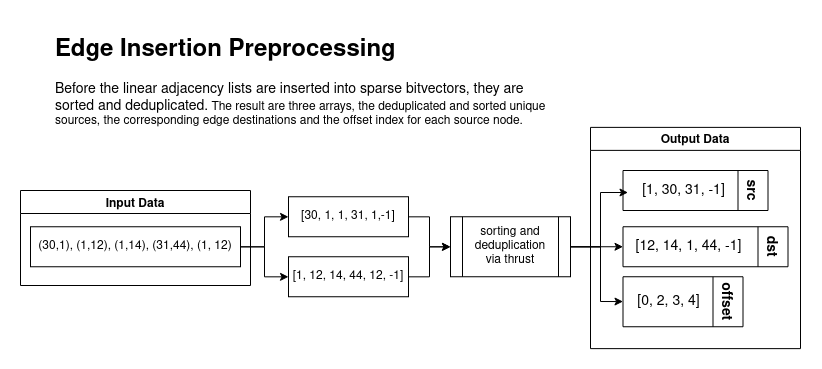
\includegraphics[width=1.\textwidth]{img/edge-insertion.png}
    \caption[Diagram for Edge Insertion]{Preprocessing of edges during edge insertion.}
    \label{fig:edge-insert}
\end{figure}
The pre-processing steps are made up of four steps, 1) the linear in-memory representation of the constraint graph is copied into device memory via \verb|cuda::memcpy| 2) all edge tuples $(src,dst)$ are sorted with $src$ as the key, 3) the algorithm iterates through all $(src,dst)$ pairs and eliminates all duplicates, 4) the algorithm iterates through all $(src,dst)$ pairs and saves the index each time src changes in a third offset array.
Since we are operating on linear memory, we can utilize the CUDA thrust library to accelerate these operations on the GPU.
Step 2 can be performed by the \verb|thrust::sort| algorithm and step 3 and 4 can be performed at the same time by \verb|thrust::unique_by_key_copy|.
One small but important detail is that before we start the pre-processing we insert a pair of \verb|UINT_MAX| values into the array for the source indices and into the array for the destination indices.
Having one additional pair assures that step 3 writes the end index for the last actual $(src,dst)$ pair into the offset array.

After the pre-processing is done, all three arrays are fed into an insertion kernel that distributes all source nodes among the available Warps, which then insert the destinations indices into the elements of the sparse bitvector.
Insertion into the element first calculates the correct base and then sets the correct bit to one if an element already exists, else a new element is first created.

\begin{figure}
    \begin{center}
        \begin{tikzpicture}[squarednode/.style={rectangle, draw=red!60, fill=red!5, very thick, minimum size=5mm}]
            \def\step{0.3}
            \node[align=left,font = {\scriptsize}] at (20*\step,9*\step) {Example insertion of an edge pair $(3,66)$.\\This is achieved by finding the correct element in the sparse\\bitvector for node index 3 and setting the correct bit to 1 for node 66.\\\\1) Calculate $base = 66/(29*32) = 0$; $word = (66\%(29*32))/32 = 2$; $bit = 66\%32 = 2$\\2) Find the \verb|head element| for node 3 by using the getIndex function from \autoref{lst:getindex}.};
            \draw [decorate,decoration = {calligraphic brace,aspect=0.28,amplitude=10pt},line width=0.5mm] (0*\step,3*\step) --  (32*\step,3*\step);
            \foreach \r in {0,2,...,31} \node at (\r*\step+0.5*\step,1.5*\step) {\tiny\r};
            \draw[step=\step] (0,0) grid (32*\step,1*\step);
            \node at (29*\step+0.5*\step,0.5*\step) {\small U};\node at (30*\step+0.5*\step,0.5*\step) {\small U};\node at (31*\step+0.5*\step,0.5*\step) {\small U};
            \node[draw,align=left,font = {\tiny}] at (40*\step,0.5*\step) {Head element in the sparse\\bitvector for node 3.};
            
            \draw (2*\step,0) -- (0,-3*\step);\draw (3*\step,0) -- (32*\step,-3*\step);
            
            \draw[step=\step] (0,-3*\step) grid (32*\step,-4*\step);
            \foreach \r in {0,...,31} \node at (\r*\step+0.5*\step,-3.5*\step) {\small1};
            \foreach \r in {0,2,...,31} \node at (\r*\step+0.5*\step,-4.5*\step) {\tiny\r};
            \node[draw,align=left,font = {\tiny}] at (40*\step,-3.5*\step) {UINT bit representation of\\2nd index in element.\\Initially all bits are set to 1.};
            \node[align=left,font = {\scriptsize}] at (19*\step,-8.5*\step) {Since the base at index 29 in the head element is uninitialized (all bits set to 1), \\we can overwrite the base with the base we calculated for node 66 in step 1.\\Additionally we set the second bit in the second word to 1.};
            
            \foreach \r in {0,2,...,31} \node at (\r*\step+0.5*\step,-12.5*\step) {\tiny\r};
            \draw[step=\step] (0,-13*\step) grid (32*\step,-14*\step);
            \node at (29*\step+0.5*\step,-13.5*\step) {\small0};\node at (30*\step+0.5*\step,-13.5*\step) {\small U};\node at (31*\step+0.5*\step,-13.5*\step) {\small U};
            \draw (2*\step,-14*\step) -- (0,-17*\step);\draw (3*\step,-14*\step) -- (32*\step,-17*\step);
            \draw[step=\step] (0,-17*\step) grid (32*\step,-18*\step);
            \foreach \r in {0,...,1} \node at (\r*\step+0.5*\step,-17.5*\step) {\small0};\node at (2*\step+0.5*\step,-17.5*\step) {\small1};\foreach \r in {3,...,31} \node at (\r*\step+0.5*\step,-17.5*\step) {\small0};
            \foreach \r in {0,2,...,31} \node at (\r*\step+0.5*\step,-18.5*\step) {\tiny\r};
            \node[draw,align=left,font = {\tiny}] at (40*\step,-15.5*\step) {After inserting the edge $(3,66)$\\into the sparse bitvector.\\Notice that the base is set\\ to 0 and both words for the next\\ index are still set to \verb|UINT_MAX|\\marked by a U.};
            \draw[-{Stealth[red]}] (2.5*\step,-15*\step) -- (2.5*\step,-16.5*\step);
        \end{tikzpicture}
    \end{center}
    \caption{An example procedure for inserting a single edge into a sparse bitvector.}
    \label{fig:edgeinsert}
\end{figure}
The previous example in \autoref{fig:edgeinsert} showcases the process for inserting a single edge into an empty sparse bitvector.
Later insertions always check whether a base is already defined in each element of the sparse bitvector and insert the edges accordingly.
The base of subsequent elements in the sparse bitvectors is always sorted in ascending order for efficient random access. To maintain the order, whenever new elements are created, for example if a given base is not yet present in a sparse bitvector, elements might have to be shifted around.
In practice these insertions are executed for each source node in parallel by multiple Warps on the GPU.

\subsection{Concurrent Graph Rewriting}\label{sec:concurrgraph}
As soon as all required edges from the constraint graph have been inserted into the correct sparse bitvectors, the Solver part of PTAGPU needs to apply the Andersen constraints from \autoref{tab:cfl-ander2} on the graph in order to calculate the correct points-to sets.
As with all calculations on the GPU we need to explicitly take care of concurrency.
Similar to edge insertion the ideal method of distributing work on the GPU is to assign units of work to individual Warps with minimal thread divergence.
When applying the production rules introduced in \autoref{tab:cfl-ander2} we can achieve this by simply using a worklist to spread out all node indices from the constraint graph across all available Warps.
This way each Warp handles the outgoing rewrite rules for a single node.
Furthermore this removes any need for specialized scheduling, because in the case that one Warp takes comparatively more time than others, the other Warps simply request new node indeces to work on.
The inherent synchronization of the worklist already takes care of optimally distributing the work.

Unfortunately we cannot simply use the production rules from the context free grammar approach in \autoref{tab:cfl-ander2}. The reason being that these rules can not be mapped onto strictly unidirectional rewrite paths in the graph.
As an example, consider the copy production rule $P\rightarrow \bar{C}P$. If we interpret this production rule in the context of graph rewriting, we get that for every node v with an outgoing copy edge to node x and an outgoing points-to edge to w, we need to add a new points-to edge from x to w.
The problem arises when multiple Warps operating on outgoing edges of different nodes, simultaneously try to mutate another node's outgoing edges.
See \autoref{fig:problem-rewrite} a) for an illustration of this problem from \cite{mendez2012gpu}.
\begin{figure}
    \centering
    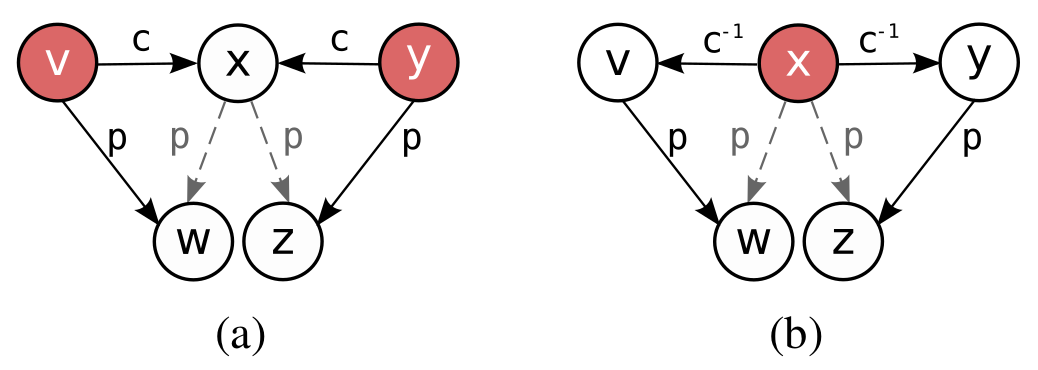
\includegraphics[width=0.5\textwidth]{img/rewriting-concurrent.png}
    \caption[Diagram for Concurrent Graph Rewriting]{Taken from \cite{mendez2012gpu}, illustrates the problem of cross node mutation when applying unmodified Andersen constraints.}
    \label{fig:problem-rewrite}
\end{figure}
A key insight from \cite{mendez2012gpu} was that, "Parallel execution of the rewrite rules \dots requires synchronization in the graph data structure.".
The intuitive solution to this problem is shown in \autoref{fig:problem-rewrite} b). For most constraints, simply inverting the edges is enough to allow for concurrent addition of new edges into the sparse bitvectors without mutatung other node's outgoing edges.
The resulting graph rewriting rules from \cite{mendez2012gpu} are listed in \autoref{tab:rewrite-rules}. These new rewrite rules can be interpreted as strictly unidirectional paths in the constraint graph.
\begin{table}
    \begin{center}
        \begin{tabular}{l|l|l}
            \hline                                                                                                                             \\
            \textbf{Statement} & \textbf{Name} & \textbf{Rewrite Rule}                                                                         \\
            \hline                                                                                                                             \\
            $x = y$            & copy          & $x \xrightarrow{c^{-1}} y \xrightarrow{p} z \mathrel{\leadsto} x \xrightarrow{p} z$           \\
            $x = *y$           & load          & $x \xrightarrow{l^{-1}} y \xrightarrow{p} z \mathrel{\leadsto} x \xrightarrow{c^{-1}} z$      \\
            $*x = y$           & store         & $x \xrightarrow{p^{-1}} y \xrightarrow{s^{-1}} z \mathrel{\leadsto} x \xrightarrow{c^{-1}} z$ \\
        \end{tabular}
    \end{center}
    \caption[List of Graph Rewriting Rules in use by PTAGPU]{Final unidirectional, partly inverted Graph Rewriting Rules proposed by \cite{mendez2012gpu}.\\Field-sensitive rules are omitted, since they are exclusively handled on the CPU, see \autoref{sec:cpugpu}.}
    \label{tab:rewrite-rules}
\end{table}
One remaining problem is, that the store rewrite rule currently require inverse point-to edge information which, if additionally stored, would greatly increase the required memory by keeping track of outgoing and incoming points-to edges at the same time for each node to allow efficient access.
The proposed solution to this problem from \cite{mendez2012gpu} is to apply the store rewrite rules in two steps. First all node pairs $(x,y)$ are collected such that y has outgoing store edges and points to x. Second all pairs with matching x are assigned to the same Warp and the resulting inverse copy edges are added to the sparse bitvectors of x, denoting the destinations of the outgoing inverse store edges from node y.
Using this method requires one additional step compared to the copy and load rules but this step can be processed very efficiently with thrust library calls, similar to the edge insertion routine.
With this two step procedure in place, we can preserve the property that each Warp only appends outgoing edges to the sparse bitvector of it's currently assigned node and refrain from explicit synchronization.
\subsubsection{Rule Application Algorithm}\label{sec:main-algo}
With both data structures and graph rewrite rules in place and optimized for operation on the GPU, the main algorithm of PTAGPU can be launched.
The pseudocode for the most important procedures of PTAGPU is available, the main loop can be found in \autoref{alg:ptagpu-main}.
\begin{algorithm}
    \caption{Main Algorithm of PTAGPU}\label{alg:ptagpu-main}
    \begin{algorithmic}
        \State \texttt{initialization steps}
        \While{\texttt{new points-to edges written into memory} $\wedge$ not done}
        \State \texttt{run updatepts kernel} \algorithmiccomment{see Algorithm 3}
        \State \texttt{launch CPU code asynchronously} \algorithmiccomment{see Algorithm 9}
        \State \texttt{run copy/load/storecollect kernel} \algorithmiccomment{see Algorithm 4}
        \State \texttt{sort $(x,y)$ pairs for the store constraints}
        \State \texttt{split pairs by unique x component}
        \State \texttt{run store kernel} \algorithmiccomment{see Algorithm 8}
        \State \texttt{await asynchronous CPU execution}
        \State \texttt{insert new edges found by CPU code}
        \State \texttt{report memory statistics and new edge count} \algorithmiccomment{optional}
        \EndWhile
        \State \texttt{free memory and pass results back to SVF}
    \end{algorithmic}
\end{algorithm}
The first step is to execute the initialization steps from \autoref{sec:init}.
Since we want to apply all rewrite rules of the Andersen style analysis until no further changes are applied, we perform the application of the rules in a while loop that breaks if no changes are detected after one iteration finishes.
We can observe the changes by counting the number of recently added points-to edges present in the newPts sparse bitvectors.
While it might seem inefficient to count through all elements in each iteration of the loop, this can be done very efficiently, since we employ massively parallel GPU kernels.
If changes to the points-to memory region have been detected, the algorithm continues with updating the newPts, currentPts and oldPts memory.
This serves the purpose of preventing redundant work, by only applying rewrite rules on the points-to edges that have been added since the last iteration.
This process is called a delta-update or diffpoints-update, the specifics of this optimization are presented in \autoref{sec:diffpts} and the pseudocode is available in \autoref{alg:ptagpu-updatepts}.
\begin{algorithm}
    \caption{Update Points Kernel}\label{alg:ptagpu-updatepts}
    \begin{algorithmic}
        \For{\texttt{each node i in constraint graph}}
        \State \texttt{traverse nextPoints sparse bitvector for node i}
        \State \texttt{collect all set bits}
        \State \texttt{compute $\Delta \mathcal{P} = nextPoints\oplus oldPoints$} \algorithmiccomment{find all new bits via xor}
        \State \texttt{update $currentPoints = \Delta \mathcal{P}$; $oldPoints = \Delta \mathcal{P} \cup oldPoints$; $newPoints = \emptyset$}
        \If{$\Delta \mathcal{P} \neq \emptyset$}
        \State \texttt{set done to $\mathbf{false}$}
        \EndIf
        \EndFor
    \end{algorithmic}
\end{algorithm}
After delta-updates are done, all points-to edges that are new since the last iteration are present in the currentPts memory region.
Before launching the first kernel for the rewrite rules, we can launch the CPU portion of our analysis asynchronously.
In practice this is realized by using C++ asynchronous futures.
See \autoref{sec:cpugpu} for the details of this forked CPU portion of the main loop.

While the asynchronous CPU code executes on a different set of CPU threads, the first GPU kernel can be launched.
The parameters for CUDA kernel launches include the block- and gridsize, as well as amount of shared memory and stream assignments.
% As PTAGPU was developed with current NVIDIA graphics cards in mind, compute capabilities 7.5 and 8.6 were targeted during compilation.
Since GPUs have a set amount of SMs that can process thread blocks in parallel, it is a good idea to split the entire body of work into at least as many thread blocks as SMs are availavble.
During development both an RTX 2080 and a RTX 3080 Ti with 48 and 82 SMs respectively were used. The PTAGPU algorithm queries the available GPUs' SM count and uses it as the gridsize.
Because the first GPU kernel processes the bulk of all rewrite rules, it heavily uses registers in each thread during execution. An individual thread requires over 128 active registers to apply the rewrite rules. As such we are limited to 64K registers per thread block per the specifications of the CUDA compute capabilities 7.0 and up. Following this hardware limitation is the fact that we can at most create 256 threads per thread block in order to not overflow the available registers per SM.
The result is a blocksize of 256, which is split into eight addressable Waps of size 32 each.

PTAGPU also includes experimental support for multi-GPU CUDA execution. This requires a unique stream per device which are initialized in the initialization steps, see \autoref{sec:init}.
This stream, together with 256 bytes of shared memory and the grid-/ blocksize specifications, make up the arguments for the first kernel launch. Later kernel launches, including the edge insertion kernel, follow the same process for finding optimal launch parameters. Furthermore CUDA provides helper functions such as \verb|cudaOccupancyMaxPotentialBlockSize| for finding the optimal grid- and blocksizes of a specific kernel.

The pseudocode for the first GPU kernel is available in \autoref{alg:ptagpu-copyload} as well as subsequent device function invocations.
\begin{algorithm}
    \caption{Copy Load Storecollect Kernel}\label{alg:ptagpu-copyload}
    \begin{algorithmic}
        \State \texttt{smem $\leftarrow$ allocate 256 bytes of shared memory per Warp}
        \State \texttt{upperlimit $\leftarrow$ totalNodeCounter}
        \State \texttt{src $\leftarrow$ incrementWorklist()}
        \While{\texttt{src < upperlimit}}
        \State \texttt{applyRewriteRule<Copy>(src,smem)} \algorithmiccomment{see Algorithm 5}
        \State \texttt{applyRewriteRule<Load>(src,smem)}
        \State \texttt{src $\leftarrow$ incrementWorklist()}
        \EndWhile
        \State \texttt{upperlimit $\leftarrow$ totalStoreCounter}
        \State \texttt{src $\leftarrow$ incrementStoreWorklist()}
        \While{\texttt{src < upperlimit}}
        \State \texttt{applyRewriteRule<CollectStore>(src,smem)} \algorithmiccomment{collect store/pts pairs for store kernel}
        \State \texttt{src $\leftarrow$ incrementStoreWorklist()}
        \EndWhile
        \State \texttt{reset worklists}
    \end{algorithmic}
\end{algorithm}
As a brief summary, the \verb|Copy Load Storecollect| kernel loops through all nodes in the constraint graph and assigns them to available Warps by using a worklist approach.
The node that is assigned to a Warp at any time is called the origin node.
As soon as a Warp receives an origin node from the constraint graph, the copy, load and the first step of the store rewrite rule are applied in this order. See \autoref{tab:rewrite-rules} for an overview of the rewrite rules that were established by \cite{mendez2012gpu}.
Each rewrite rule is applied by a template function, see \autoref{alg:ptagpu-applyrewrite}.
\begin{algorithm}
    \caption[applyRewriteRule Procedure Pseudocode]{\texttt{template<Type> applyRewriteRule} procedure\\
        \begin{minipage}[t]{0.1\textwidth}
            \textbf{Input:}
        \end{minipage}
        \begin{minipage}[t]{0.8\textwidth}
            src: currently processing node\\
            smem: shared memory
        \end{minipage}
    }\label{alg:ptagpu-applyrewrite}
    \begin{algorithmic}
        \State \texttt{index $\leftarrow$ getIndex(src)}
        \Repeat
        \State \texttt{bits $\leftarrow$ memory[index + threadIdx.x]}
        \State \texttt{collectBitvectorTargets<Type>(src,bits,smem)} \algorithmiccomment{see Algorithm 6}
        \State \texttt{index $\leftarrow$ nextBits}
        \Until{\texttt{index $\neq$ ULLONG\_MAX}}
        \If{\texttt{Type = StoreCollect}}
        \State \texttt{insert all pairs $(src,smem[:])$ into store map} \algorithmiccomment{later used in the store kernel}
        \Else
        \State \texttt{mergeBitvectors(src,smem)} \algorithmiccomment{see Algorithm 7}
        \EndIf
    \end{algorithmic}
\end{algorithm}
Template functions are a C++ construct that allows using placeholder parameters. Each function invocation with different template parameters results in a different symbol during compilation. While using templates in C++ is good practice for writing reusable, efficient, and error-free code, here we use the fact that CUDA supports templates in device function to prevent the PTX compiler from assuming recursion and falsely limiting the available number of threads to prevent register exhaustion.

Inside the \verb|applyRewriteRule| function, depending on the current rewrite rule, the destinations of all outgoing edges of a certain type are collected by the \verb|collectBitvectorTargets| function, see \autoref{alg:ptagpu-collectbv}.
\begin{algorithm}
    \caption[collectBitvectorTargets Procedure Pseudocode]{\texttt{template<Type> collectBitvectorTargets} procedure\\
        \begin{minipage}[t]{0.1\textwidth}
            \textbf{Input:}
        \end{minipage}
        \begin{minipage}[t]{0.8\textwidth}
            to: currently processing node\\
            bits: of the head element in to's sparse bitvector\\
            smem: shared memory
        \end{minipage}
    }\label{alg:ptagpu-collectbv}
    \begin{algorithmic}
        \If{\texttt{bits $\neq$ 0}}
        \For{\texttt{i = 0\dots 31}}
        \If{\texttt{(1<<i) $\wedge$ bits}} \algorithmiccomment{check if bit is set}
        \State \texttt{target $\leftarrow$ base * (29*32) + threadIdx.x * 32 + i}
        \State \texttt{append target to smem} \algorithmiccomment{target represents the destination of the edge}
        \EndIf
        \EndFor
        \EndIf
    \end{algorithmic}
\end{algorithm}
The destinations of the outgoing edges are collected by traversing the correct sparse bitvector of the origin node, element by element.
Following this, all outgoing edges of the collected destination nodes are merged with the outgoing edges of the current origin node of the Warp.
For example, applying the copy rewrite rule $origin \xrightarrow{c^{-1}} y \xrightarrow{p} z \mathrel{\leadsto} origin \xrightarrow{p} z$ PTAGPU first collects all targets of the outgoing inverse copy edges, then merges all the outgoing points-to edges from the collected nodes with the outgoing points-to edges of the origin node.
This is realized by the \verb|mergeBitvectors| function, see \autoref{alg:ptagpu-mergebv}, at the end of the \verb|applyRewriteRule| function.
\begin{algorithm}
    \caption[mergeBitvectors Procedure Pseudocode]{\texttt{mergeBitvectors} procedure\\
        \begin{minipage}[t]{0.1\textwidth}
            \textbf{Input:}
        \end{minipage}
        \begin{minipage}[t]{0.8\textwidth}
            to: node that outgoing edges are merged into\\
            smem: array of nodes whose outgoing edges are to be merged with to
        \end{minipage}
    }\label{alg:ptagpu-mergebv}
    \begin{algorithmic}
        \For{\texttt{from $\leftarrow$ smem}}
        \State \texttt{toIndex $\leftarrow$ getIndex(to)} \algorithmiccomment{find the index of the head element}
        \State \texttt{fromIndex $\leftarrow$ getIndex(from)}
        \While{\texttt{next element $\neq$ ULLONG\_MAX}}
        
        \If{\texttt{fromBase = toBase}}
        \State \texttt{merge element at fromIndex into toIndex}
        \ElsIf{\texttt{fromBase < toBase}}
        \State \texttt{insert new element before toIndex} \algorithmiccomment{elements are sorted by base}
        \Else
        \If{\texttt{toIndex has next element}}
        \State \texttt{toIndex $\leftarrow$ toNext}
        \Else
        \State \texttt{create new element after toIndex and insert fromIndex}
        \EndIf
        \EndIf
        
        \State \texttt{toIndex $\leftarrow$ toNext} \algorithmiccomment{read next elements in sparse bitvectors}
        \State \texttt{fromIndex $\leftarrow$ fromNext}
        \EndWhile
        \EndFor
    \end{algorithmic}
\end{algorithm}
In principle the bitwise merging of two sparse bitvectors works exactly the same as during edge insertion, shown in \autoref{fig:edgeinsert}, during initialization.
Notably, applying the storeCollect rewrite rule, does not merge any sparse bitvectors, but instead collects store and points-to pairs which are later processed in another kernel for the reasons outlined in the beginning of \autoref{sec:concurrgraph}.
After all rewrite rules are applied and worklists are reset, the first kernel execution concludes.

Following the first kernel execution in \autoref{alg:ptagpu-copyload}, the store and points-to pairs previously collected are preprocessed by the thrust library, see \autoref{fig:edge-insert} for an overview of the preprocessing steps, and then fed into the second GPU kernel \autoref{alg:ptagpu-store} where the last rewrite rule is finally applied.
\begin{algorithm}
    \caption[Store Kernel Pseudocode]{Store Kernel}\label{alg:ptagpu-store}
    \begin{algorithmic}
        \State \texttt{smem $\leftarrow$ allocate 256 bytes of shared memory per Warp}
        \For{\texttt{some x of collected $(x,y)$ pts/$\text{store}^{-1}$ pairs}}
        \For{\texttt{each unique y of collected $(x,y)$ pts/$\text{store}^{-1}$ pairs}}
        \State \texttt{append y to smem}
        \EndFor
        \State \texttt{mergeBitvectors(x,smem)} \algorithmiccomment{see Algorithm 7}
        \EndFor
    \end{algorithmic}
\end{algorithm}

After the second and final kernel execution, we await the conclusion of the asynchronous CPU procedure.
Since the CPU procedure stores all new edges it finds in pair of vectors, representing the adjacency information of all new edges, we can insert all new edges into the sparse bitvectors by reusing the edge insertion code during initialization.

At the end of each iteration of the main loop PTAGPU optionally presents the current memory usage and distribution among the memory regions for debugging end evaluation purposes. This includes statistics for the elapsed time of each component in PTAGPU - as measured by the C++ chrono\footnote{\url{https://en.cppreference.com/w/cpp/chrono}} library.

\subsubsection{Diffpoints Updates}\label{sec:diffpts}
If the main loop of PTAGPU were to repeatedly iterate and apply the same rewrite rules on every node, every iteration would repeat the work of the previous operation, making the algorithm very inefficient.
This problem does not only apply to PTAGPU, all pointer analyses need to prevent excessive repeating of already finished work.
As such many implementations use a concept called diffpoints or delta-updates that is meant to prevents redundant work. Also pointer analyses inside SVF make use of diffpoints in order to speed up the calculations.
Diffpoints work by dividing the points-to relations calculated during application of the constraints into separate sets.
One set describing all new edges that are calculated in the current iteration, one set for all points-to edges calculated in the previous iteration and one set for the bulk of all prior points-to edges.
As can be seen in \autoref{alg:ptagpu-updatepts}, the update process between iterations be be realized by simple set operations or more optimized bitwise operations.
$$\Delta \mathcal{P} = nextPoints\oplus oldPoints$$
$$currentPoints = \Delta \mathcal{P}\wedge oldPoints = \Delta \mathcal{P} \cup oldPoints\wedge newPoints = \emptyset$$
After the update at the beginning of each iteration, all procedures apply the rewrite rules on the $\mathtt{currentPoints}$ set.
With diffpoints in place we can ensure that each rewrite rule is only processed once, since any points-to edges are only in the set $\mathtt{currentPoints}$ exactly once.

One problem that arises from using diffpoints, is the fact that whenever a new copy edge is added into the constraint graph - which can happen dynamically by applying rewrite rules - the next iteration does not process all points-to edges that need to be considered because of the addition of the copy edge. Instead, only those points-to edges are processed, which are in $\mathtt{currentPoints}$. The straightforward solution to this problem is to always explicitly work through all points-to edges in $\mathtt{coldPoints}$ whenever a new copy edge is added.
This ensures that no points-to edges are skipped during processing.
\subsection{Combining CPU and GPU}\label{sec:cpugpu}
PTAGPU strives to achieve optimal concurrent execution.
This includes not only all GPU cores, but also all CPU cores.
To achieve this, parts of the main loop, see \autoref{alg:ptagpu-main}, are split into an asynchronous CPU execution.
This asynchronous CPU part is implemented with async futures.
Async futures are a feature of the C++ programming language that allows for the implementation of asynchronous programming. Asynchronous programming allows for the concurrent execution of multiple tasks within a single program, enabling improved efficiency and scalability. By using async futures, developers can write code that can take advantage of multiple cores or perform time-consuming tasks without blocking the main thread of the program. This can greatly improve the performance of C++ programs, especially on systems with multiple CPU cores or heterogenous compute capabilities. See the following basic example in \autoref{lst:asynccpu}.

\begin{listing}
    \begin{minted}{c++}
    // Launch an asynchronous task
    std::future<int> result = std::async([]() {
        // Perform some long-running computation
        int sum = 0;
        for (int i = 0; i < 1000000000; ++i)
        {
            sum += i;
        }
        return sum;
    });

    // Do something else in the meantime
    std::cout << "Hello, world!" << std::endl;

    // Wait for the asynchronous task to complete
    int final_result = result.get();
    std::cout << "The final result is: " << final_result << std::endl;
    \end{minted}
    \caption{C++ Sample illustrating Async Futures}
    \label{lst:asynccpu}
\end{listing}

To further improve the scalability of the CPU portion of PTAGPU, the asynchronously executed code is parallelized using OpenMP pragmas.
The pseudocode for the CPU code is available in \autoref{alg:ptagpu-cpu}.
\begin{algorithm}
    \caption[CPU Async Procedure Pseudocode]{\texttt{CPU async} procedure}\label{alg:ptagpu-cpu}
    \begin{algorithmic}
        \State \texttt{typedef pair<vector<uint>,vector<uint>> edgeSet} \algorithmiccomment{\small type for adjacency information\normalsize}
        \Procedure{\texttt{asyncCPU}}{\texttt{edgeSet *ptsSet, edgeSet *copySet}}
        \State \texttt{\#pragma omp parallel for num\_threads(16)}
        \For{\texttt{each GEP edge in constraint graph}}
        \State \texttt{dstPTS $\leftarrow \emptyset$ }
        \State \texttt{srcPTS $\leftarrow$ collectBitvectorTargets<PTS>(edge.src)}
        \For{\texttt{id in srcPTS}}
        \State \texttt{fieldOffsetNode $\leftarrow$ consCG->getGepObjVar(id, edge.offset)}
        \State \texttt{\#pragma omp critical} \algorithmiccomment{only executed by one thread at a time}
        \State \texttt{append fieldOffsetNode to dstPTS}
        \EndFor
        \State \texttt{\#pragma omp critical}
        \For{\texttt{id in dstPTS}}
        \State \texttt{addPts(edge.dst,id)}
        \EndFor
        \EndFor
        \State \texttt{updateCallGraph(getIndirectCallsites())} \algorithmiccomment{these are SVF superclass methods}
        \State \texttt{// some of getIndirectCallsites's internal function calls are}
        \State \texttt{// overwritten to use unified memory instead of SVF data structures}
        \EndProcedure
    \end{algorithmic}
\end{algorithm}
As we do not make use of multiple CPU cores in any other part of the program, we can utilize a majority of the available CPU cores for the async execution.
The calculation that is performed on the CPU reads the available points-to information to resolve all getelementpointer, edges in the constraint graph.
While other GPU implementations of Andersen's analysis, such as \cite{mendez2012gpu}, also perform the gep calculations on the GPU, this leaves the CPU mostly idle during the execution.
Furthermore paralellizing the application of gep constraints is not as easily done for the copy, load and store constraints, since each gep instruction carries an offset value. Given the offset value and the points-to target of a node we need to calculate the correct abstract memory object that the offset references. This can be done on the GPU as demonstrated by \cite{mendez2012gpu}, but is more efficient to implement on a CPU, since gep instructions can reference random regions in memory.
Beyond difficult synchronization on a GPU, it is also ideal to use the CPU for gep constraint resolution, since PTAGPU is directly integrated into SVF, which already offers a variety of optimized methods for gep constraint resolution.
Lastly the asynchronous CPU code also resolves all indirect callsites and updates the callgraph. 
Arguably this is one of the most important aspects of PTAGPU that differentiates it from other implementations of Andersen's analysis on the GPU.
Indirect callsite resolution is often omitted from academic implementations like \cite{mendez2012gpu}, \cite{zuo2021systemizing} or \cite{su2014parallel}.
Since an over-approximated callgraph is one of the fundamental results of a pointer analysis next to points-to information as described in \autoref{sec:svf}, resolving indirect callsites is an important step for the analyis to be usable by further analyses inside SVF.
\subsection{Feeding the Results back into SVF}\label{sec:feedingback}
At some point PTAGPU concludes its calculation and has produced a constraint graph inside unified memory, which includes an over-approximation of the points-to set for each pointer variable.
On its own the constraint graph in the form of sparse bitvectors is not digestible by SVF. For this reason an interface is created to enable SVF to use the points-to information produced by SVF.
Internally the \verb|PointerAnalysis| superclass inside SVF provides an \verb|alias| method that takes two node indices and outputs the alias relation of both nodes.
To provide pointer information for SVF, PTAGPU overwrites the alias method with its own implementation that reads points-to edges from the sparse bitvectors inside unified memory and outputs one of the possible alias relations from \autoref{eq:alias1} and \autoref{eq:alias2}.
One of the consumers of this information is the SVF test suite\footnote{\url{https://github.com/SVF-tools/Test-Suite}} which will be used in \autoref{sec:testsuite} for verifying the results PTAGPU produces against a know corpus of test programs that include various pointer relations.

Beyond points-to information, the \verb|updateCallGraph| method in \autoref{alg:ptagpu-cpu}, which resolves indirect callsites, also requires access to the points-to information of PTAGPU. To facilitate this, some of the SVF implementations for callsite resolution are overwritten in PTAGPU to redirect the reading of points-to information into the unified memory.
The benefit of using C++ polymorphism to overwrite these internal methods from SVF is that the points-to information can remain in unified memory and does not have to be explicitly written back into main memory.
This improves performance without impeding the functions of SVF.
\section{Experimental Results}
To validate PTAGPU in termns of correctness and performance various test cases and benchmark programs were used.
Following, the experimental results are split into correctness testing and performance testing.
While for correctness testing a pre defined test suite was used, a collection of current open source programs of varying complexity was compiled for real world performance testing.

\subsection{Test Suite}\label{sec:testsuite}
For correctness testing the PTABENCH\footnote{\url{https://github.com/SVF-tools/Test-Suite}}, a sub project of the SVF framework, was used.
The PTABENCH repository includes a set of small test programs that are compiled into LLVM bitcode. These test programs contain a set of constraints that represent a state that should be reached by the repsective analyses.
The test suite implements unit tests for all variants of pointer analysis included in SVF as well as more complex analyses, such as memory leak detection and multithreaded flow analyses. 
Part of the test corpus are specific edge cases that test quirks of real programs, such as SPEC CPU2000, in order to ensure all analyses produce sound results.
As part of PTAGPU, testing with PTABENCH was enabled to apply the unit tests and test whether or not sound results are produced.
This was achieved by overwriting parts of the test invocation implementation inside SVF as alluded to in \autoref{sec:feedingback}.

The constraints in the test programs are implemented as function calls that relay the meaning of each property that is to be checked by the test case. The functions do not have to be defined for the constraint to be checked.
When one of these special function calls is encountered at the end of the analysis, an alias check is performed for both function parameters.
This check directly reads the points-to relations from unified memory and reports whether both variables may alias or are in fact not aliased.
Note that the lack of precision of our whole program analysis prevents us from making any definitive statements about whether or not two variables have to alias, only that they may alias. For this reason any must alias constraints are interpreted as may alias constraints in our pointer analysis.
As an example, see the following test program in \autoref{lst:testcase} that checks whether a pointer analysis in SVF correctly resolves load and store constraints.

\begin{listing}
    \begin{minted}{c}
    int main()
    {
        int a,b,*c,*d;
        c = &a;
        d = &a;
        MUSTALIAS(c,d); // c and d may alias each other
        NOALIAS(&b,d); // the address of b and d must not alias
    }
        \end{minted}
    \caption{A unit test in the PTABENCH test suite.}
    \label{lst:testcase}
\end{listing}

\begin{listing}
    \begin{minted}{bash}
    for i in Test-Suite/test_cases_bc/basic_c**/*; 
        do build/ptagpu/runptagpu -stat=0 $i ; 
        if [ $? -ne 0 ]; then
            # break
        fi
    done
    \end{minted}
    \caption{Sample bash script for applying all unit tests on PTAGPU.}
    \label{lst:testbash}
\end{listing}

When executing the PTABENCH test suite while using PTAGPU as the pointer analysis backend, all 107 unit tests applicable to pointer analyses successfully produce the expected results with regards to pointer and indirect callsite information.
The results can be replicated within the source code either by applying the test suite manually with a simple bash script like the one in \autoref{lst:testbash} or by using the CTest library of CMAKE and building the \verb|test| target.
From this it is concluded that PTAGPU produces sound, field-sensitive pointer analysis results and does not reduce the accuracy of other pointer analyses in SVF in any way.
Interestingly, the current state of the art pointer analysis implementation of SVF, the Andersen based wave propagation algorithm with diffpoints, successfully analyzes only 106 of the 107 unit tests.
This discrepancy was not further investigated.

\subsection{Benchmark Suite}
To assess the performance of PTAGPU and establish a set of metrics that can be compared to other pointer analysis implementations, a suite of open source projects was compiled and used as input for pointer analyses.
The collection of open source projects was selected to present a diverse set of code bases in terms of code style and size of the programs.
The collection consists of 16 programs, each varying in complexity. See \autoref{tab:benchmarkprograms} for an overview of all the selected benchmark programs.
As PTAGPU and SVF rely on the LLVM project for data generation and input in the form of compiled bitcode, the selection of benchmark programs is somewhat limited to those written in languages for which LLVM compiler frontends exist. This includes programming languages such as C, C++, Rust, Fortran, and many other systems programming languages.

The evaluation was performed on PTAGPU, the proposed algorithm of this thesis, and both the Andersen based wave propagation algorithm and the naive Andersen analysis of SVF.
The Andersen wave propagation algorithm represents a highly optimized current state of the art inclusion-based, field-sensitive, context- and flow-insensitive pointer analysis.
Furthermore the results will showcase the differences between sequential CPU implemantations and parallel GPU implementations.

\begin{table}
    \centering
    \begin{tabular}{||c c c c S[table-format = 1.3,retain-zero-exponent=true] c||}
        \hline
        program       & \#V  & \#E  & bc size & {density} & avg. degree \\
        \hline\hline
        nano          & 6    & 2    & 298K    & 5.887e-05 & 0.399       \\ 
        diff          & 54   & 17   & 1.3M    & 5.794e-06 & 0.317       \\
        httpd         & 169  & 95   & 1.4M    & 3.180e-05 & 0.561       \\
        htop          & 48   & 20   & 1.6M    & 8.447e-06 & 0.413       \\
        zstd          & 280  & 101  & 2.3M    & 6.260e-05 & 0.362       \\
        bison         & 146  & 59   & 3.4M    & 1.417e-05 & 0.407       \\
        redis         & 207  & 67   & 4.8M    & 6.507e-04 & 0.327       \\
        perl          & 445  & 206  & 4.9M    & 1.617e-04 & 0.464       \\
        linux-minimal & 393  & 157  & 5.4M    & 7.872e-03 & 0.401       \\
        bash          & 238  & 77   & 5.4M    & 7.514e-05 & 0.327       \\
        vim           & 696  & 280  & 7.7M    & 7.676e-05 & 0.403       \\
        postgres      & 1432 & 721  & 18M     & 2.642e-04 & 0.504       \\
        python        & 742  & 313  & 21M     & 3.453e-04 & 0.422       \\
        git           & 869  & 379  & 25M     & 3.399e-03 & 0.437       \\
        php           & 1582 & 611  & 52M     & 1.689e-04 & 0.386       \\
        linux         & 4464 & 2206 & 72M     & 5.629e-04 & 0.494       \\
        \hline
    \end{tabular}
    \caption{List of benchmark programs used to evaluate PTAGPU.\\Number of nodes in thousands, number of edges in thousands, bitcode filesize in kilobytes, density and average out degree for each constraint graph.}
    \label{tab:benchmarkprograms}
\end{table}

\subsubsection{Methodology}
To generate the bitcode for the pointer analyses, each of the 16 benchmark projects was compiled with the clang\footnote{\url{https://clang.llvm.org}} compiler. During compilation for each object that was compiled and assembled, equivalant bitcode was generated which was then linked along with the object code to produce both a binary - or a set of binaries, depending on the project - and a bitcode file for the entire program.
Instead of manually intercepting each compile operation for each source file, the wllvm\footnote{\url{https://github.com/travitch/whole-program-llvm}} utility was used which is specifically designed to extract whole program bitcode from source packages by injecting bticode generating compiler flags during the build process.
Since most of the selected benchmark programs use common open source toolchains, such as Makefiles and bootstrapping scripts, the custom wllvm compiler interface was specified through either standard environment variables  \verb|CC| and  \verb|CXX| or arguments to the configure scripts.
Each of the resulting bitcode files are provided together with the source code of PTAGPU.
Furthermore, if a given project provided a test suite, that test suite was used to verify the functions of the compiled program to ensure that the compilation successfully produced a working binary, bitcode pair. 

After the bitcode was generated, it was used as input for all three pointer analysis algorithms via a driver program that loads the bitcode into memory, initializes SVF and executes the correct pointer analysis.
All analyses that were evaluated were compiled with gcc and the optimization flag \verb|-O2|.
Each analysis was performed 5 times to ensure the results are consistent and reliable and not falsified by external factors. This was necessary, since one of the hardware setups was part of a shared server.
The individual time measurements were performed by using the C++ chrono\footnote{\url{https://en.cppreference.com/w/cpp/chrono}} library.

\subsubsection{Hardware Setup}
Three separate machines were used to evaluate the pointer analyses.
Machine A was equipped with a 12 core AMD Ryzen 5900x CPU, 32GiB of memory and an NVIDIA RTX 3080Ti, machine B was equipped with two sockets of 16 core Intel Xeon Gold 6242 processors capable of simultaneous multithreading, 1.5 TiB of memory and 8 NVIDIA RTX 2080 GPUs and machine C was a cloud instance equipped with 256 vCPUs and an A100 GPU with 80GiB of HBM2 memory.
Because some of the larger programs in the benchmark suite exceeded the 32 GiB of system memory on machine A during analysis, the reported results were mostly gathered on machine B, except for TODO where the effect of the amount of available SMs on different GPUs was evaluated.
To test how much the larger benchmark programs benefit from more graphics memory, those benchmarks that require more memory that available on the RTX 3080Ti and RTX 2080 were executed on machine C as well.

\subsubsection{Results}
Initially the PTAGPU analysis and both Andersen based pointer analyses, wavediff and naive-ander, were executed on machine B. The results of which can be found in \autoref{tab:benchmarkresults} where the runtimes of all three analyses are reported in elapsed seconds from beginning to end of each analysis.
\begin{table}
    \centering
    \begin{tabular}{||c S[table-format = 5.3] S[table-format = 4.3] S S[table-format = 5.3] r||}
        \hline
        program      & {t-wavediff} & {t-ptagpu} & {speedup} & {t-naive-ander} & {GPU memory}            \\
        \hline\hline
        bash         & 16.222       & 15.489     & 1.05      & 102195.752      & \qty{1024}{\mebi\byte}  \\
        bison        & 18.977       & 9.837      & 1.93      & 119999.054      & \qty{260}{\mebi\byte}   \\
        diff         & 1.469        & 4.231      & 0.35      & 1561.577        & \qty{71}{\mebi\byte}    \\
        git          & 557.953      & 4690.010   & 0.12      & 33404492.853    & \qty{21467}{\mebi\byte} \\
        htop         & 2.912        & 5.275      & 0.55      & 5696.107        & \qty{93}{\mebi\byte}    \\
        httpd        & 5.321        & 6.414      & 0.83      & 2889.208        & \qty{160}{\mebi\byte}   \\
        nano         & 0.087        & 1.751      & 0.05      & 98.5            & \qty{7}{\mebi\byte}     \\
        perl         & 103.338      & 45.093     & 2.29      & 2688610.846     & \qty{3999}{\mebi\byte}  \\
        php          & 645.697      & 64965.400  & 0.01      & 6530636.248     & \qty{27561}{\mebi\byte} \\
        postgres     & 997.355      & 465.527    & 2.14      & 6481597.401     & \qty{16430}{\mebi\byte} \\
        python       & 536.515      & 203.649    & 2.63      & 1731373.999     & \qty{9016}{\mebi\byte}  \\
        redis-server & 8.679        & 11.592     & 0.75      & 4834.759        & \qty{207}{\mebi\byte}   \\
        vim          & 1052.995     & 268.628    & 3.92      & {-$^b$}         & \qty{11966}{\mebi\byte} \\
        vmlinux      & 32100.566    & {-$^a$}    & {-$^a$}   & {-$^a$}         & {-$^a$}                 \\
        vmlinux-tiny & 91.479       & 188.315    & 0.49      & 1410004.628     & \qty{2175}{\mebi\byte}  \\
        zstd         & 11.063       & 13.172     & 0.84      & 7958.999        & \qty{454}{\mebi\byte}   \\
        \hline
    \end{tabular}
    \caption{Benchmark results comparing PTAGPU, Andersen wavediff and naive Andersen analysis measured in seconds. Executed on machine B.\\The $^a$ denotes that the analysis did not finish in under 10 hours.\\The $^b$ denotes that the analysis failed to compute a solution.}
    \label{tab:benchmarkresults}
\end{table}
The results from machine B showed that the PTAGPU analysis had a high speedup (greater than 2) for several programs, including "perl", "python", "postgres", and "vim", indicating that it was significantly faster than the wavediff analysis for these programs. However, the PTAGPU analysis had a low speedup (less than 0.5) for several programs, including "diff", "git", "nano" and "php", indicating that it was noticably slower than the wavediff analysis for these programs.
Most of the programs with small speedups are smaller in terms of node and edge count of the constraint graph, such as "diff", "htop", "nano" and "zstd". These slow results for the smaller programs can be explained by the overhead associated with CUDA initializations. For example the PTAGPU analysis for the nano program took 1687 ms, where 1533 ms were spent on CUDA memory allocations and deallocations and 145 ms on the actual kernels. Comparing this to the 87 ms required for the wavediff analysis, the PTAGPU analysis runtime is dominated by overhead from the CUDA memory management. This explains the relatively slow performance of PTAGPU on the smaller benchmarks.
Notably the results for the benchmarks "git" and "php" achieved an especially low speedup of 0.12 and 0.01 respectively, although both programs are relatively large and the analysis was not dominated by CUDA memory management but the primary kernel instead, see \autoref{fig:stackedbar-problem}, indicating a large workload on the GPU.
\begin{figure}
    \centering
    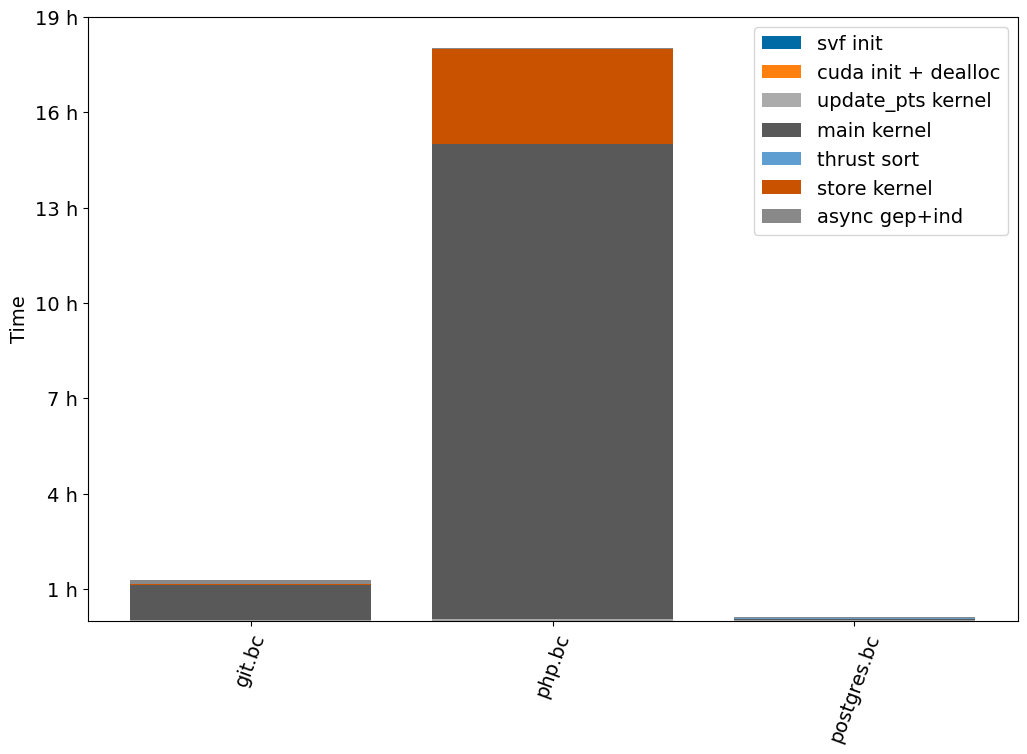
\includegraphics[width=.6\textwidth]{img/stackedbar-problems.png}
    \caption[Stacked bar graph for PTAGPU runtime on git, postgres and php benchmarks.]{Stacked bar graph for PTAGPU runtime on git, postgres and php benchmarks in a memory constrained environment.}
    \label{fig:stackedbar-problem}
\end{figure}
Looking at the third graph in \autoref{fig:correlations}, it is clear that exceeding the 12 GiB of graphics memory available per GPU on machine B has a disproportionally negative effect on performance.
This can be attributed to the fact that allocating more unified memory than available graphics memory leads to an excess of page faults, as soon as the grahpics memory is exhausted during migration from the CPU to the GPU. 
While this could be mitigated by prefetching only the required memory regions into the GPU memory on-demand during analysis, this would require partitioning the sparse bitvectors into chunks that fit into graphics memory, which is not trivially done for larger analyses.
\begin{figure}
    \centering
    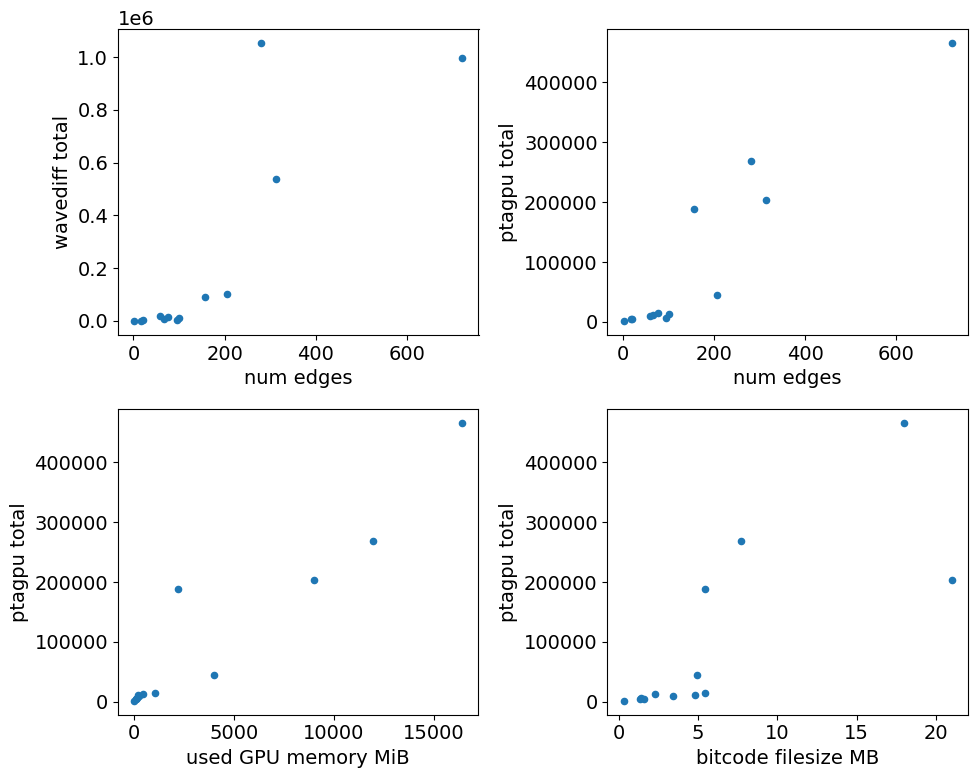
\includegraphics[width=.9\textwidth]{img/correlations.png}
    \caption{Detailed statistics from machine B.}
    \label{fig:correlations}
\end{figure}
To verify that the performance impact was caused by pagefaults in the CUDA driver, the \verb|strace| tool was used to inspect the system calls during the PTAGPU analysis of the php program, which showed \verb|ioctl| system calls to and from the CUDA unified memory address space.

To further evaluate the performance of the PTAGPU algorithm without being memory constrained, machine C was used to analyze the benchmark programs with PTAGPU again. Using the NVIDIA A100 GPU on machine C, all analyses except vmlinux fit into the 80 GiB of graphics memory. The results of the second benchmarks can be found in \autoref{tab:benchmarkresults-a100}.
\begin{table}
    \centering
    \begin{tabular}{||c S[table-format = 5.3] S[table-format = 3.3] S r||}
        \hline
        program      & {t-wavediff} & {t-ptagpu-a100} & {speedup} & {GPU memory}             \\
        \hline\hline
        bash         & 16.222       & 13.126          & 1.23      & \qty{1024.0}{\mebi\byte} \\
        bison        & 18.977       & 7.599           & 2.49      & \qty{260}{\mebi\byte}    \\
        diff         & 1.469        & 3.305           & 0.44      & \qty{71}{\mebi\byte}     \\
        git          & 557.953      & 869.302         & 0.64      & \qty{21467}{\mebi\byte}  \\
        htop         & 2.912        & 4.039           & 0.72      & \qty{93}{\mebi\byte}     \\
        httpd        & 5.321        & 4.720           & 1.12      & \qty{160}{\mebi\byte}    \\
        nano         & 0.087        & 1.626           & 0.05      & \qty{7}{\mebi\byte}      \\
        perl         & 103.338      & 41.854          & 2.46      & \qty{3999}{\mebi\byte}   \\
        php          & 645.697      & 500.086         & 1.29      & \qty{27561}{\mebi\byte}  \\
        postgres     & 997.355      & 290.219         & 3.43      & \qty{16430}{\mebi\byte}  \\
        python       & 536.515      & 172.701         & 3.10      & \qty{9016}{\mebi\byte}   \\
        redis-server & 8.679        & 8.830           & 0.98      & \qty{207}{\mebi\byte}    \\
        vim          & 1052.995     & 247.859         & 4.24      & \qty{11966}{\mebi\byte}  \\
        vmlinux      & 32100.566    & {-$^c$}         & {-$^c$}   & {-$^c$}                  \\
        vmlinux-tiny & 91.479       & 136.164         & 0.67      & \qty{2175}{\mebi\byte}   \\
        zstd         & 11.063       & 9.795           & 1.12      & \qty{454}{\mebi\byte}    \\
        \hline
    \end{tabular}
    \caption{Benchmark results comparing PTAGPU, Andersen wavediff and naive Andersen analysis measured in seconds. Executed on machine C.\\The $^a$ denotes that the analysis did not finish in under 10 hours.\\The $^b$ denotes that the analysis failed to compute a solution.\\The $^c$ denotes that the analysis ran out of memory.}
    \label{tab:benchmarkresults-a100}
\end{table}

The benchmarks on the A100 overall improved the performance of PTAGPU, increasing the speedup factor for all programs.
Specifically the "git", "php", "postgres" and "python" benchmarks improved the most, since the analysis was not limited by GPU memory.
Depending on the benchmark program, PTAGPU was up to four times faster than the wavediff algorithm. Compared to the naive implementation of Andersen's algorithm in SVF PTAGPU was several orders of magnitude faster on every one of the benchmarks.
At its slowest PTAGPU was about 50\% as fast as the wavediff algorithm.
\begin{figure}
    \centering
    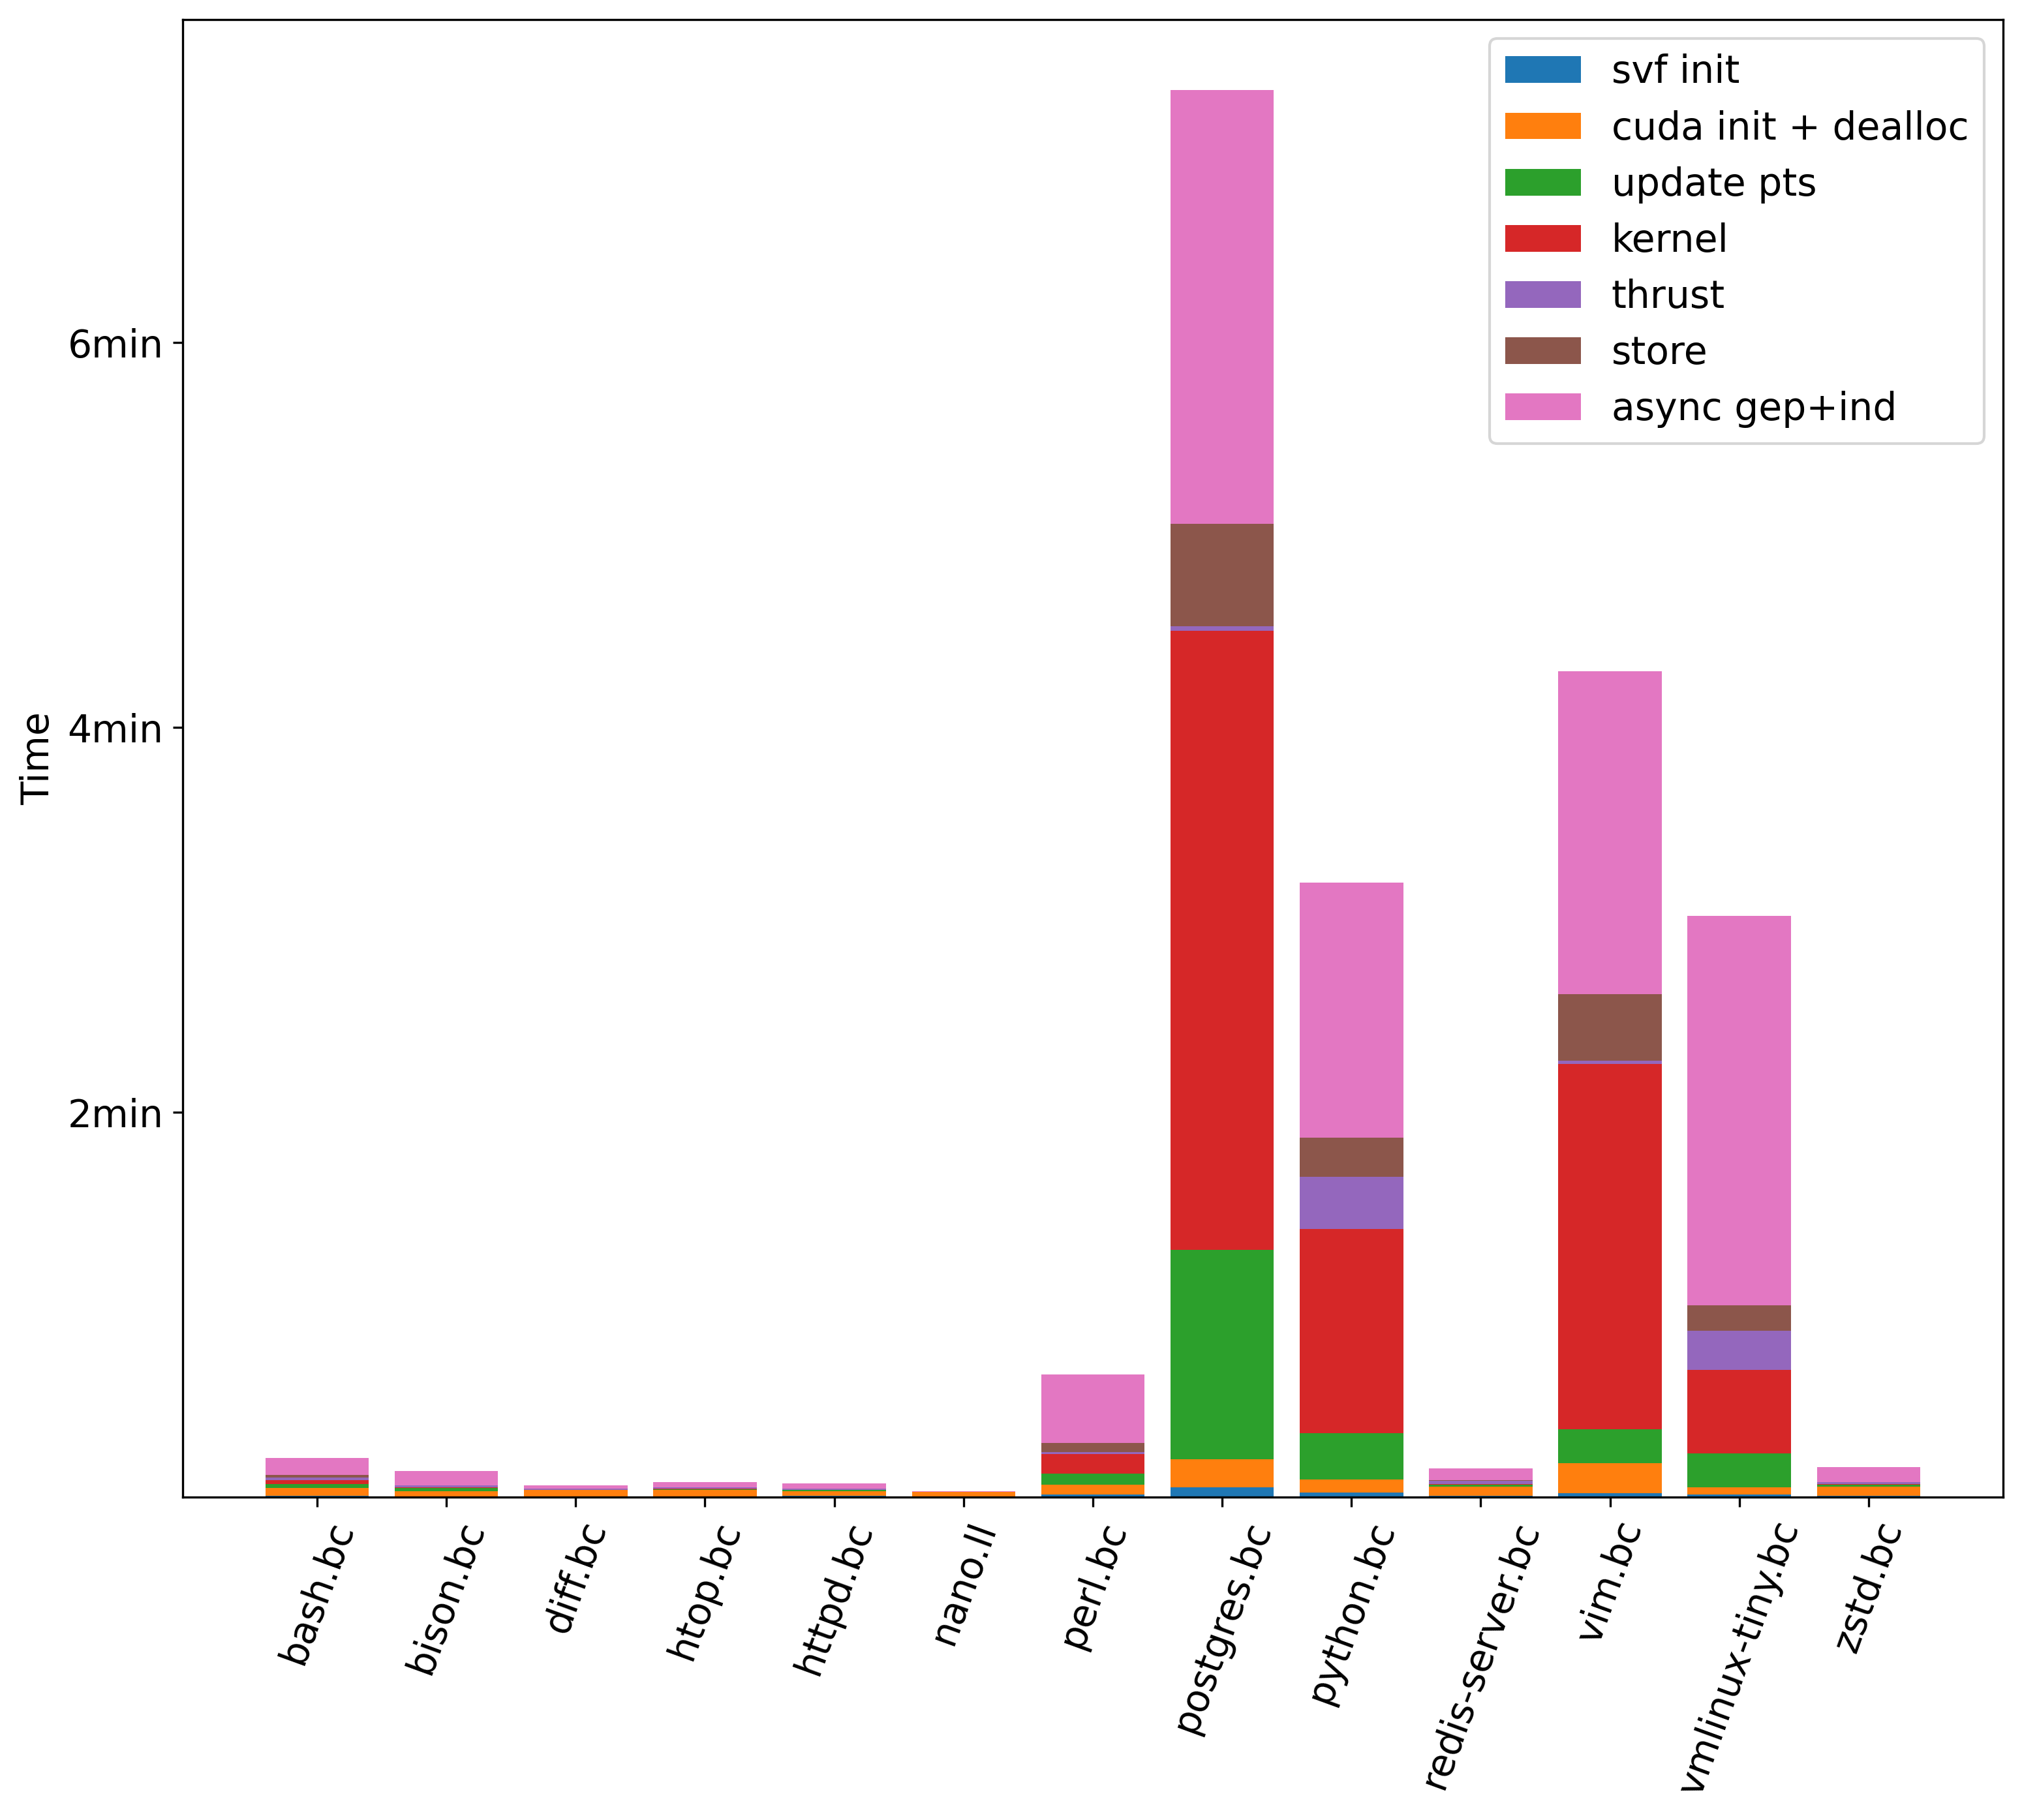
\includegraphics[width=.9\textwidth]{img/stackedbar.png}
    \caption{stacked bar graph}
    \label{fig:stackedbar}
\end{figure}

\begin{figure}
    \centering
    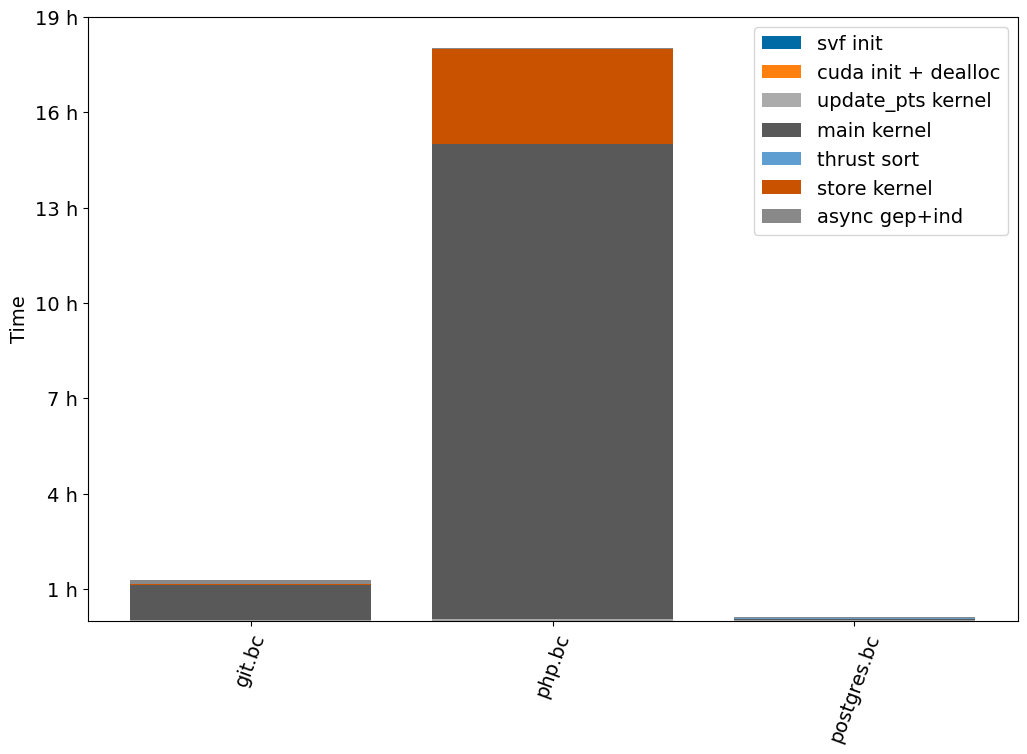
\includegraphics[width=.9\textwidth]{img/stackedbar-problems.png}
    \caption{stacked bar graph for problematic results}
    \label{fig:stackedbar-problem}
\end{figure}

\begin{figure}
    \centering
    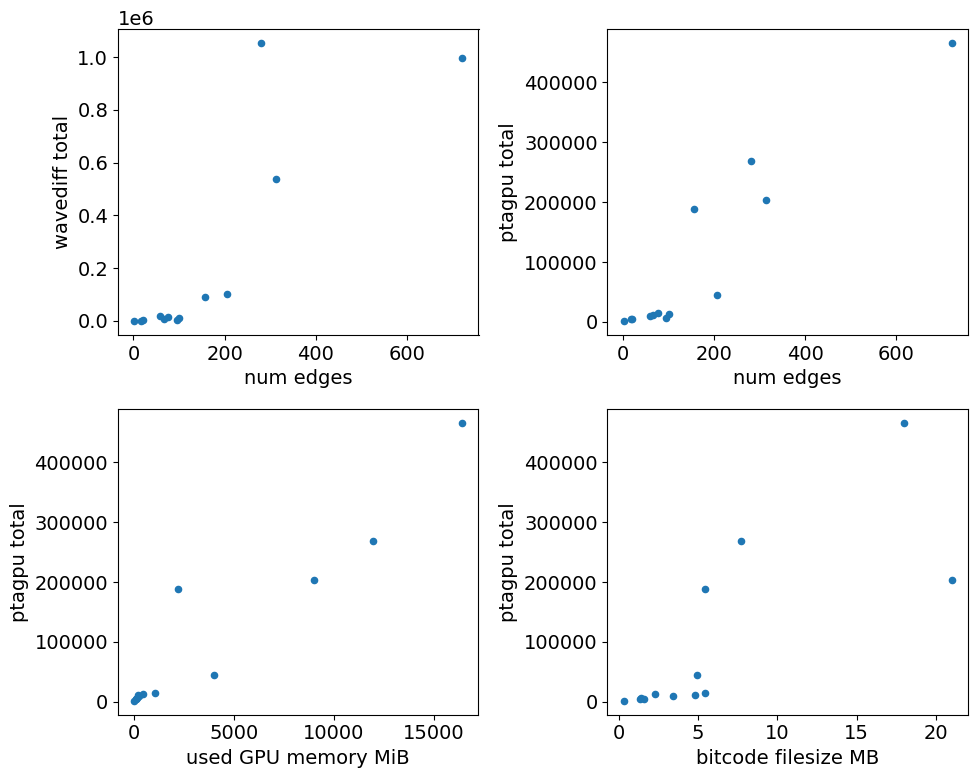
\includegraphics[width=.9\textwidth]{img/correlations.png}
    \caption{ignoring memory constrained benchmarks, correlations between runtime and memory usage}
    \label{fig:correlations}
\end{figure}

\begin{figure}
    \centering
    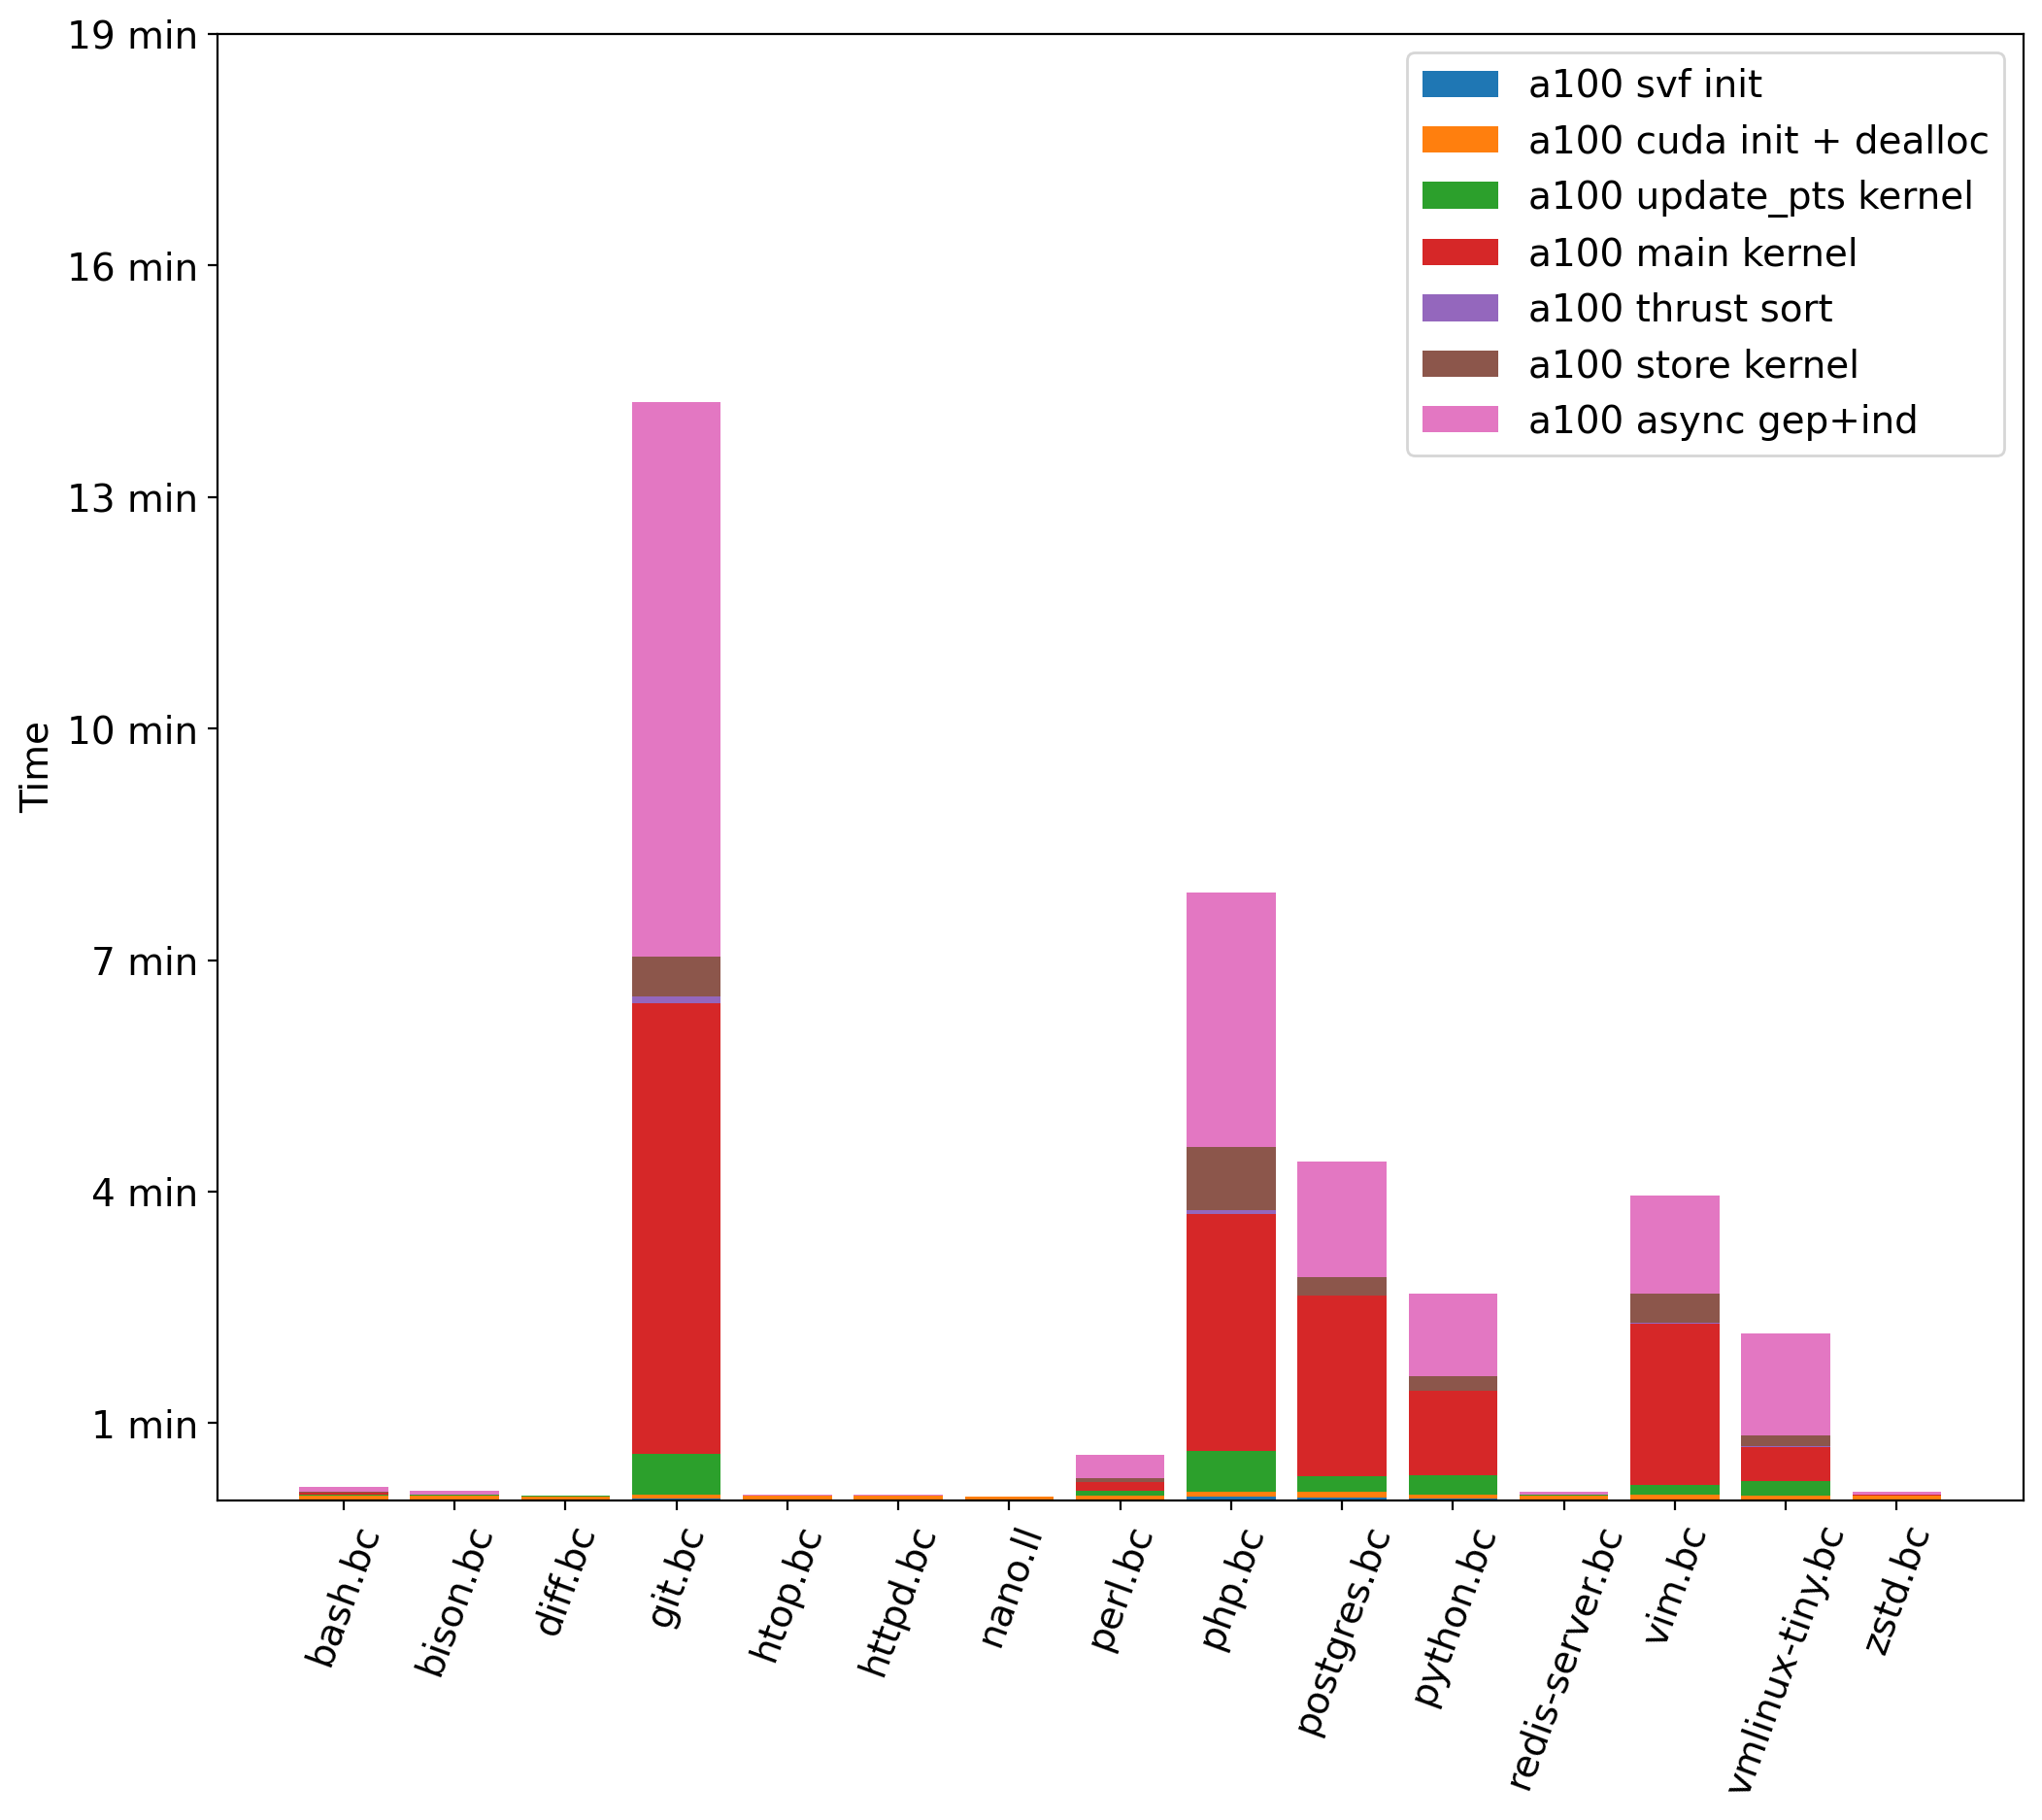
\includegraphics[width=.9\textwidth]{img/stackedbar-a100.png}
    \caption{stacked bar graph on a100}
    \label{fig:stackedbar-a100}
\end{figure}

\begin{figure}
    \centering
    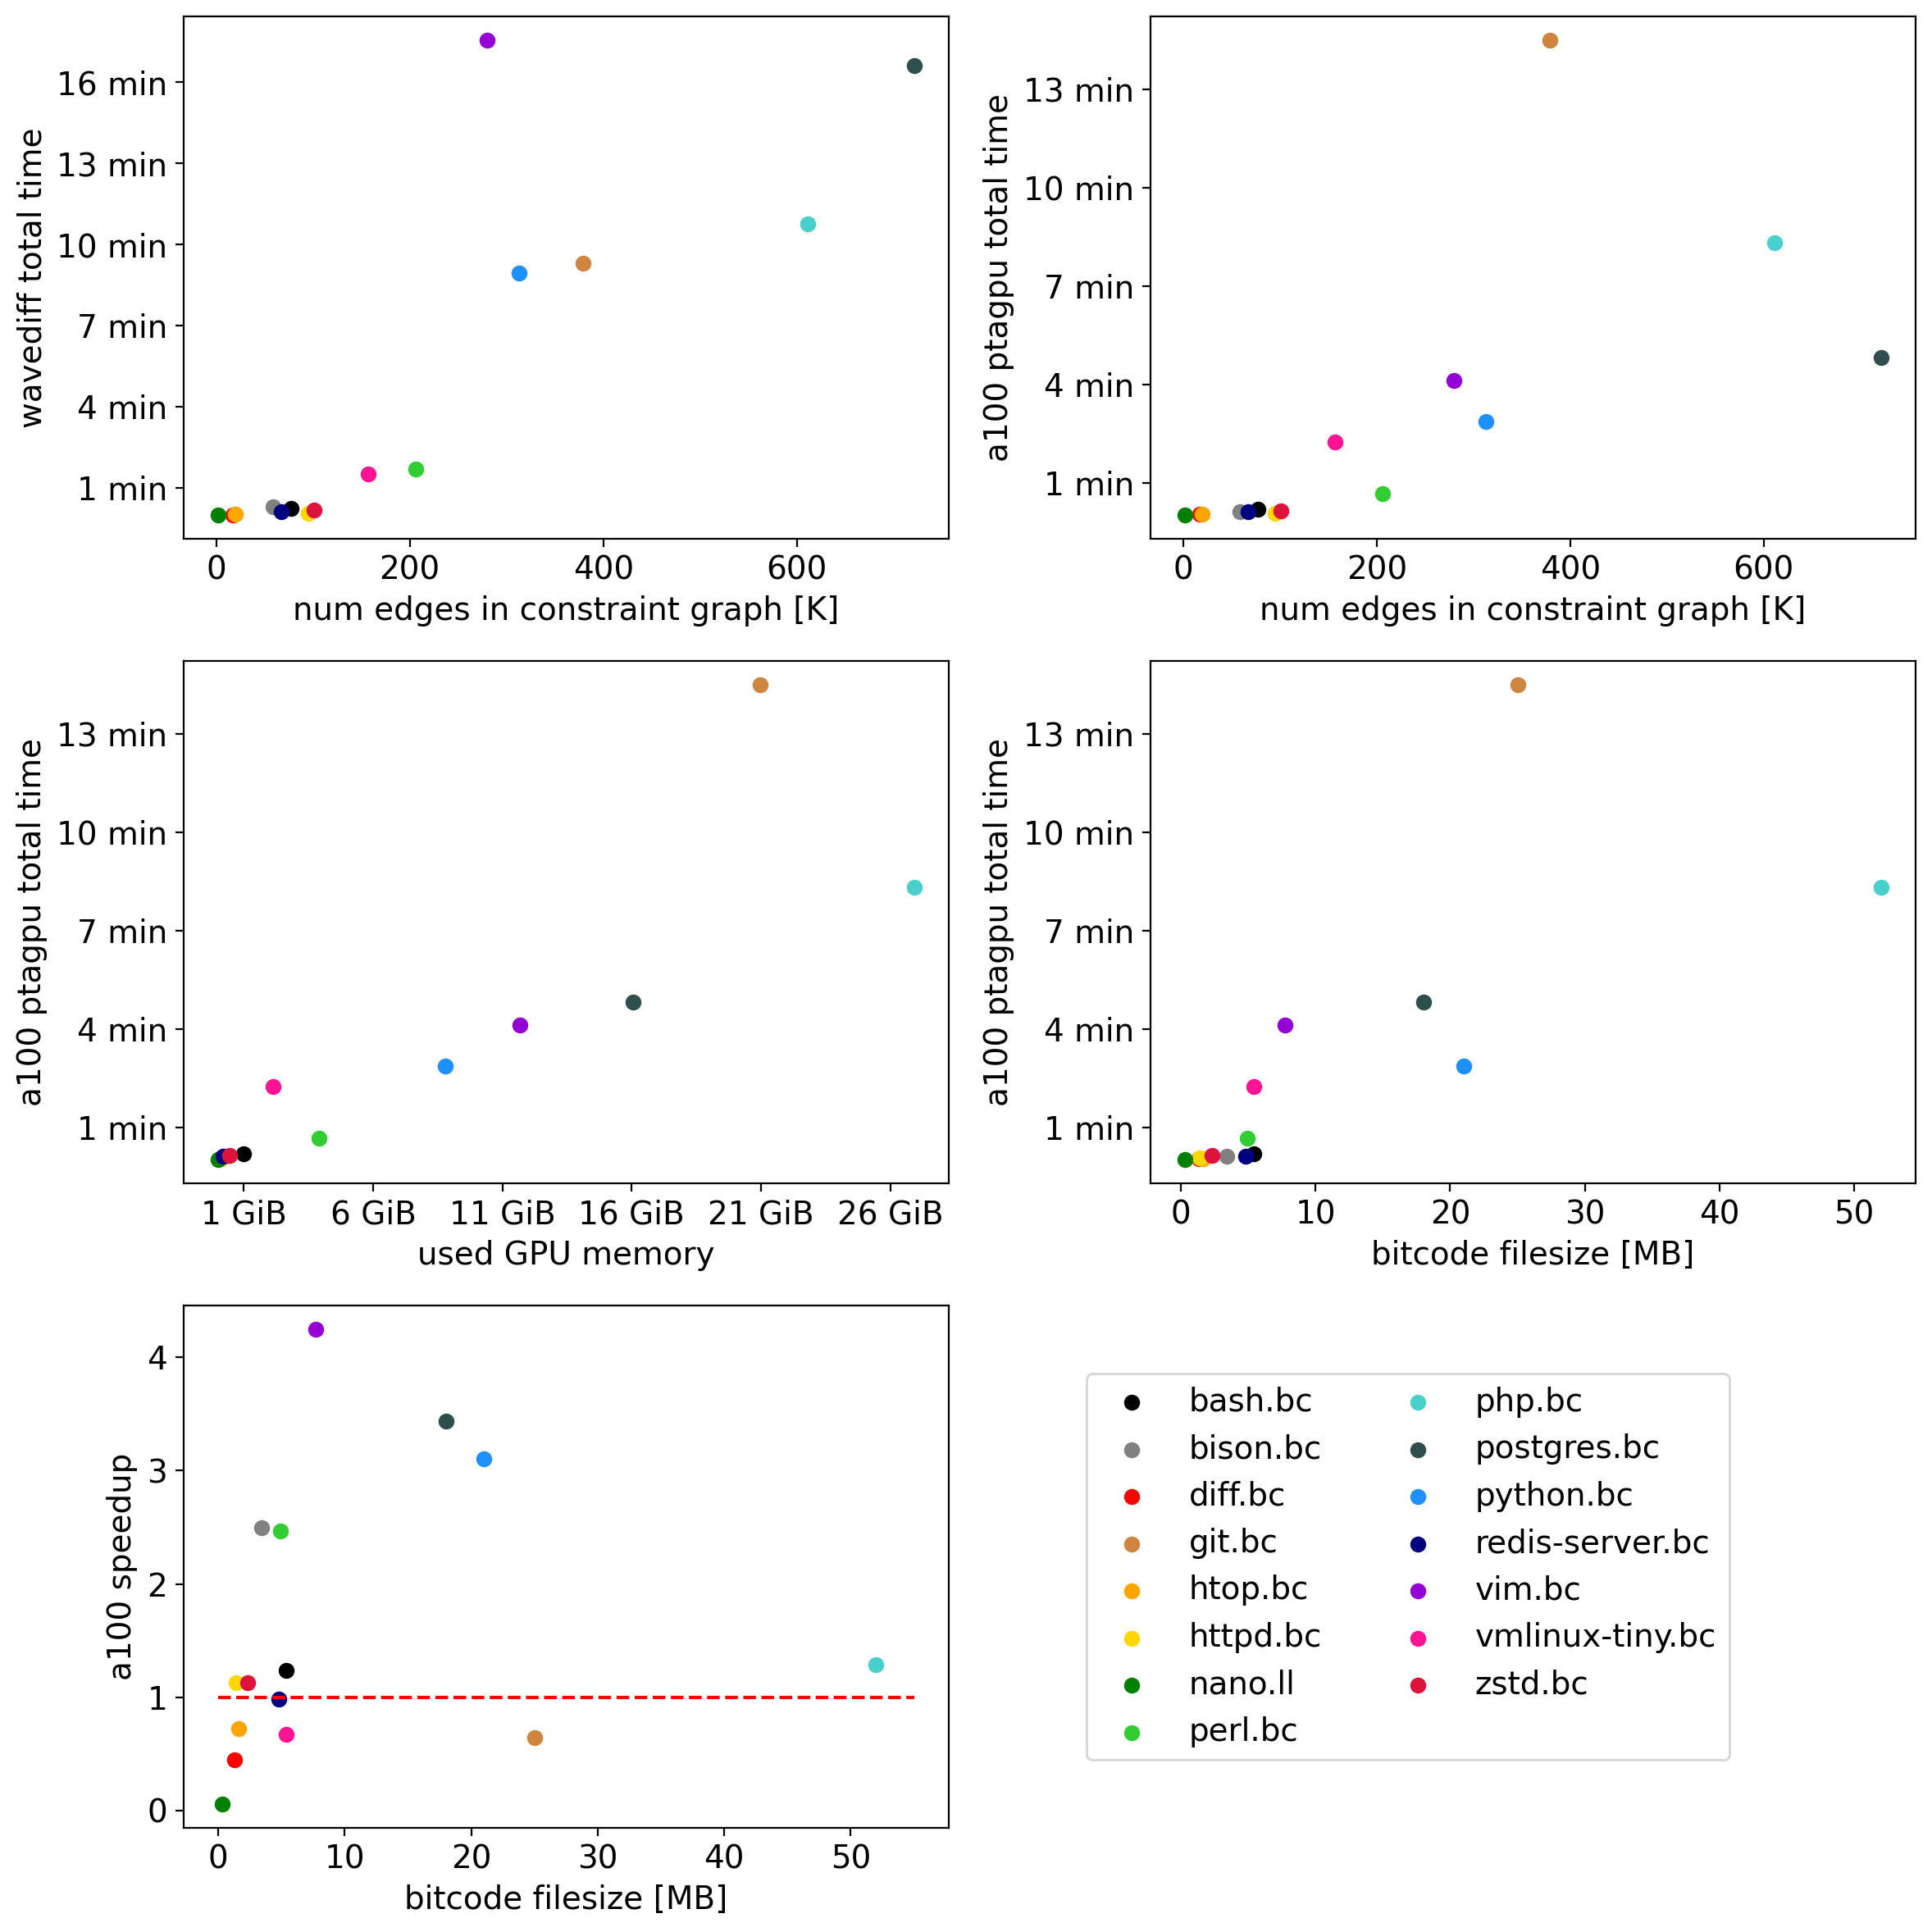
\includegraphics[width=.9\textwidth]{img/correlations-a100.png}
    \caption{correlations between runtime and other stuff on a100}
    \label{fig:correlations-a100}
\end{figure}

\section{Evaluation}

\chapter{Conclusion}\label{chap:conclusion}

\section{Evaluation of Results}
To summarize the research conducted up to this point, a GPU-supported parallel Andersen based pointer analysis, PTAGPU was implemented on top of LLVM and the SVF framework using the NVIDIA CUDA SDK.
PTAGPU was both tested for correctness and performance in comparison to established CPU-based pointer analyses in multiple benchmarks and hardware combinations.
The primary research question was to what extent such an implementation presents advantages or disadvantages over other analyses that are not strictly parallel in nature.

The experimental results presented in \autoref{sec:results} indicate that PTAGPU is a viable implementation to improve the performance of a whole program field-sensitive pointer analysis without sacrificing precision of the analysis.
PTAGPU achieved an average speedup of 1.60 across 15 benchmarks over the SVF wavediff algorithm. Since the individual benchmarks with lower speedups are almost entirely smaller programs, the absolute time saved by using PTAGPU was 28 minutes and 59 seconds over the total 1 hour 07 minutes and 30 seconds required by wavediff to analyze all 16 programs. In terms of absolute time, the speedup factor was 1.75.
This represents a meaningful improvement over the CPU algorithm. 
Unfortunately this does not include the linux benchmark, as the analysis did not fit into graphics memory and did not finish within a reasonable amount of time.
Although enough unified memory was available, the analyis of the linux source code did become impeded by excessive page faults as illustrated in \autoref{sec:results}.
Judging from the wavediff analysis of the linux kernel, roughly 300 GiB of memory are required for a successful whole program field-sensitive pointer analysis, which is currently impossible to compute on a single GPGPU.

One key insight from the experimental results was, that there are no trivial prior indicators for analysis runtime, since program structure are seemingly more influential on analysis runtime than lines of code, nodes in the constraint graph or size of the compiled program.
This is supported by prior research from \cite{mendez2012gpu}, where the selected benchmark programs - some of which overlap with the selected benchmark programs of this thesis - also had vastly different speedups for the GPU-based analysis over the CPU-based analyses. 

Although the results indicate that PTAGPU generally outperforms the CPU counterparts in larger benchmarks, it should be acknowledged that it is difficult to establish a fair comparison betwenn CPU and GPU pointer analysis implementations.
Both in terms of upfront cost and power consumption both implementations are vastly different. While the SVF wavediff algorithm can be executed on almost any modern computer with sufficient main memory, PTAGPU requires specialized hardware. Especially for larger analyses, a GPU with enough graphics memory is required for an efficient analysis with PTAGPU.

\section{Future Work}
\subsection{Partitioning Workloads}
\subsection{Hybrid Cycle Detection}
\section{Discussion}

\appendix

\chapter{Raw Data}

\begin{table}[h]
    \tiny
    \begin{tabular}{rrrrrrrr}
        \toprule
           & file         & GPU memory MiB & filesize MB & wavediff-t   & naiveander-t & num nodes [K] & num edges [K] \\
        \midrule
        1  & bash         & 1024           & 5.400       & 16222.113    & 102195.752   & 238           & 77            \\
        2  & bison        & 260            & 3.400       & 18977.376    & 119999.054   & 146           & 59            \\
        3  & diff         & 71             & 1.300       & 1469.056     & 1561.577     & 54            & 17            \\
        4  & git          & 21467          & 25.000      & 557953.924   & 33404492.853 & 869           & 379           \\
        5  & htop         & 93             & 1.600       & 2912.693     & 5696.107     & 48            & 20            \\
        6  & httpd        & 160            & 1.400       & 5321.631     & 2889.208     & 169           & 95            \\
        7  & nano         & 7              & 0.298       & 87.438       & 98.500       & 6             & 2             \\
        8  & perl         & 3999           & 4.900       & 103338.824   & 2688610.846  & 445           & 206           \\
        9  & php          & 27561          & 52.000      & 645697.175   & 6530636.248  & 1582          & 611           \\
        10 & postgres     & 16430          & 18.000      & 997355.718   & 6481597.401  & 1432          & 721           \\
        11 & python       & 9016           & 21.000      & 536515.479   & 1731373.999  & 742           & 313           \\
        12 & redis-server & 207            & 4.800       & 8679.144     & 4834.759     & 207           & 67            \\
        13 & vim          & 11966          & 7.700       & 1052995.525  & NaN          & 696           & 280           \\
        14 & vmlinux      & NaN            & 72.000      & 32100566.652 & NaN          & 4464          & 2206          \\
        15 & vmlinux-tiny & 2175           & 5.400       & 91479.697    & 1410004.628  & 393           & 157           \\
        16 & zstd         & 454            & 2.300       & 11063.214    & 7958.999     & 280           & 101           \\
        \bottomrule
    \end{tabular}

    \caption{Raw Data of Baseline results for wavediff and naiveander Pointer Analyses}
\end{table}

\begin{table}[h]
    \tiny
    \begin{tabular}{rrrrrrrrrr}
        \toprule
           & ptagpu-t    & svf init & cuda init & update-k   & main-k       & thrust sort & store-k      & async CPU  & S    \\
        \midrule
        1  & 15489.00    & 366.515  & 2489.389  & 1129.063   & 1324.698     & 743.670     & 858.932      & 5190.693   & 1.05 \\
        2  & 9837.06     & 214.357  & 1650.840  & 830.177    & 234.046      & 675.748     & 54.633       & 4317.114   & 1.93 \\
        3  & 4231.58     & 66.945   & 2065.479  & 103.057    & 33.120       & 379.843     & 23.591       & 953.283    & 0.35 \\
        4  & 4690010.00  & 2190.250 & 17095.315 & 70148.000  & 3968158.215  & 11743.372   & 68373.295    & 538454.710 & 0.12 \\
        5  & 5275.51     & 68.425   & 2053.573  & 229.714    & 202.955      & 433.321     & 41.092       & 1587.968   & 0.55 \\
        6  & 6414.69     & 309.354  & 1481.509  & 303.996    & 42.605       & 511.057     & 8.219        & 1637.408   & 0.83 \\
        7  & 1751.01     & 7.732    & 1533.113  & 1.829      & 3.040        & 45.140      & 1.057        & 94.275     & 0.05 \\
        8  & 45093.40    & 775.915  & 2939.635  & 3457.350   & 6125.819     & 767.334     & 2751.206     & 21457.059  & 2.29 \\
        9  & 64965400.00 & 2809.670 & 20928.407 & 193679.543 & 53783100.092 & 12298.489   & 10732741.786 & 187398.213 & 0.01 \\
        10 & 465527.00   & 2911.590 & 8824.470  & 65379.251  & 192989.575   & 1374.555    & 32019.477    & 135372.093 & 2.14 \\
        11 & 203649.00   & 1344.910 & 4088.639  & 14380.164  & 63762.440    & 16295.704   & 12199.745    & 79598.063  & 2.63 \\
        12 & 11592.50    & 357.262  & 2785.032  & 688.684    & 95.318       & 1158.755    & 42.613       & 3688.319   & 0.75 \\
        13 & 268628.00   & 1166.830 & 9292.169  & 10709.775  & 113872.762   & 947.744     & 20876.445    & 100689.414 & 3.92 \\
        14 & NaN         & NaN      & NaN       & NaN        & NaN          & NaN         & NaN          & NaN        & NaN  \\
        15 & 188315.00   & 654.966  & 2405.784  & 10600.173  & 25890.805    & 12319.814   & 7893.207     & 121492.773 & 0.49 \\
        16 & 13172.60    & 388.764  & 2791.627  & 680.571    & 90.320       & 687.799     & 80.554       & 4526.521   & 0.84 \\
        \bottomrule
    \end{tabular}
    \caption{Raw Data of PTAGPU on Machine B}
\end{table}

\begin{table}[h]
    \tiny
    \begin{tabular}{rrrrrrrrrr}
        \toprule
           & ptagpu-t   & svf init & cuda init & update-k  & main-k     & thrust sort & store-k   & async CPU  & S    \\
        \midrule
        1  & 13126.316  & 316.589  & 3339.273  & 955.132   & 1258.228   & 103.923     & 824.671   & 3404.405   & 1.23 \\
        2  & 7599.453   & 181.425  & 3397.507  & 657.559   & 203.553    & 92.256      & 41.323    & 2941.927   & 2.49 \\
        3  & 3304.592   & 53.196   & 3119.867  & 100.198   & 29.448     & 73.122      & 13.813    & 379.511    & 0.44 \\
        4  & 869302.000 & 1489.250 & 2852.620  & 31480.079 & 350891.929 & 4856.937    & 30923.576 & 431554.218 & 0.64 \\
        5  & 4038.684   & 58.770   & 3238.629  & 212.349   & 189.568    & 74.528      & 20.536    & 852.136    & 0.72 \\
        6  & 4720.701   & 233.173  & 3125.778  & 258.309   & 39.757     & 57.139      & 5.049     & 848.704    & 1.12 \\
        7  & 1626.456   & 5.655    & 3163.307  & 2.024     & 4.073      & 8.778       & 0.786     & 18.179     & 0.05 \\
        8  & 41853.936  & 644.417  & 3277.899  & 3452.222  & 6873.348   & 164.523     & 2906.182  & 18027.103  & 2.46 \\
        9  & 500086.000 & 2561.200 & 3815.678  & 32016.810 & 184075.139 & 2797.468    & 49062.434 & 198397.500 & 1.29 \\
        10 & 290219.000 & 2465.070 & 4439.149  & 12040.787 & 140270.103 & 211.504     & 14064.883 & 89735.395  & 3.43 \\
        11 & 172701.000 & 1088.500 & 3468.036  & 14790.821 & 65522.991  & 203.848     & 11336.972 & 63986.167  & 3.10 \\
        12 & 8830.066   & 247.339  & 3339.556  & 615.407   & 103.871    & 109.152     & 24.580    & 2143.869   & 0.98 \\
        13 & 247859.000 & 963.959  & 3336.741  & 7599.231  & 125708.265 & 123.820     & 23102.001 & 75995.761  & 4.24 \\
        14 & NaN        & NaN      & NaN       & NaN       & NaN        & NaN         & NaN       & NaN        & NaN  \\
        15 & 136164.602 & 554.447  & 3152.182  & 11286.157 & 26563.670  & 236.409     & 8721.936  & 79417.327  & 0.67 \\
        16 & 9795.036   & 312.077  & 3104.891  & 546.614   & 70.509     & 75.957      & 61.621    & 2587.828   & 1.12 \\
        \bottomrule
    \end{tabular}
    \caption{Raw Data of PTAGPU on Machine C}
\end{table}
\normalsize

\begin{figure}[h]
    \centering
    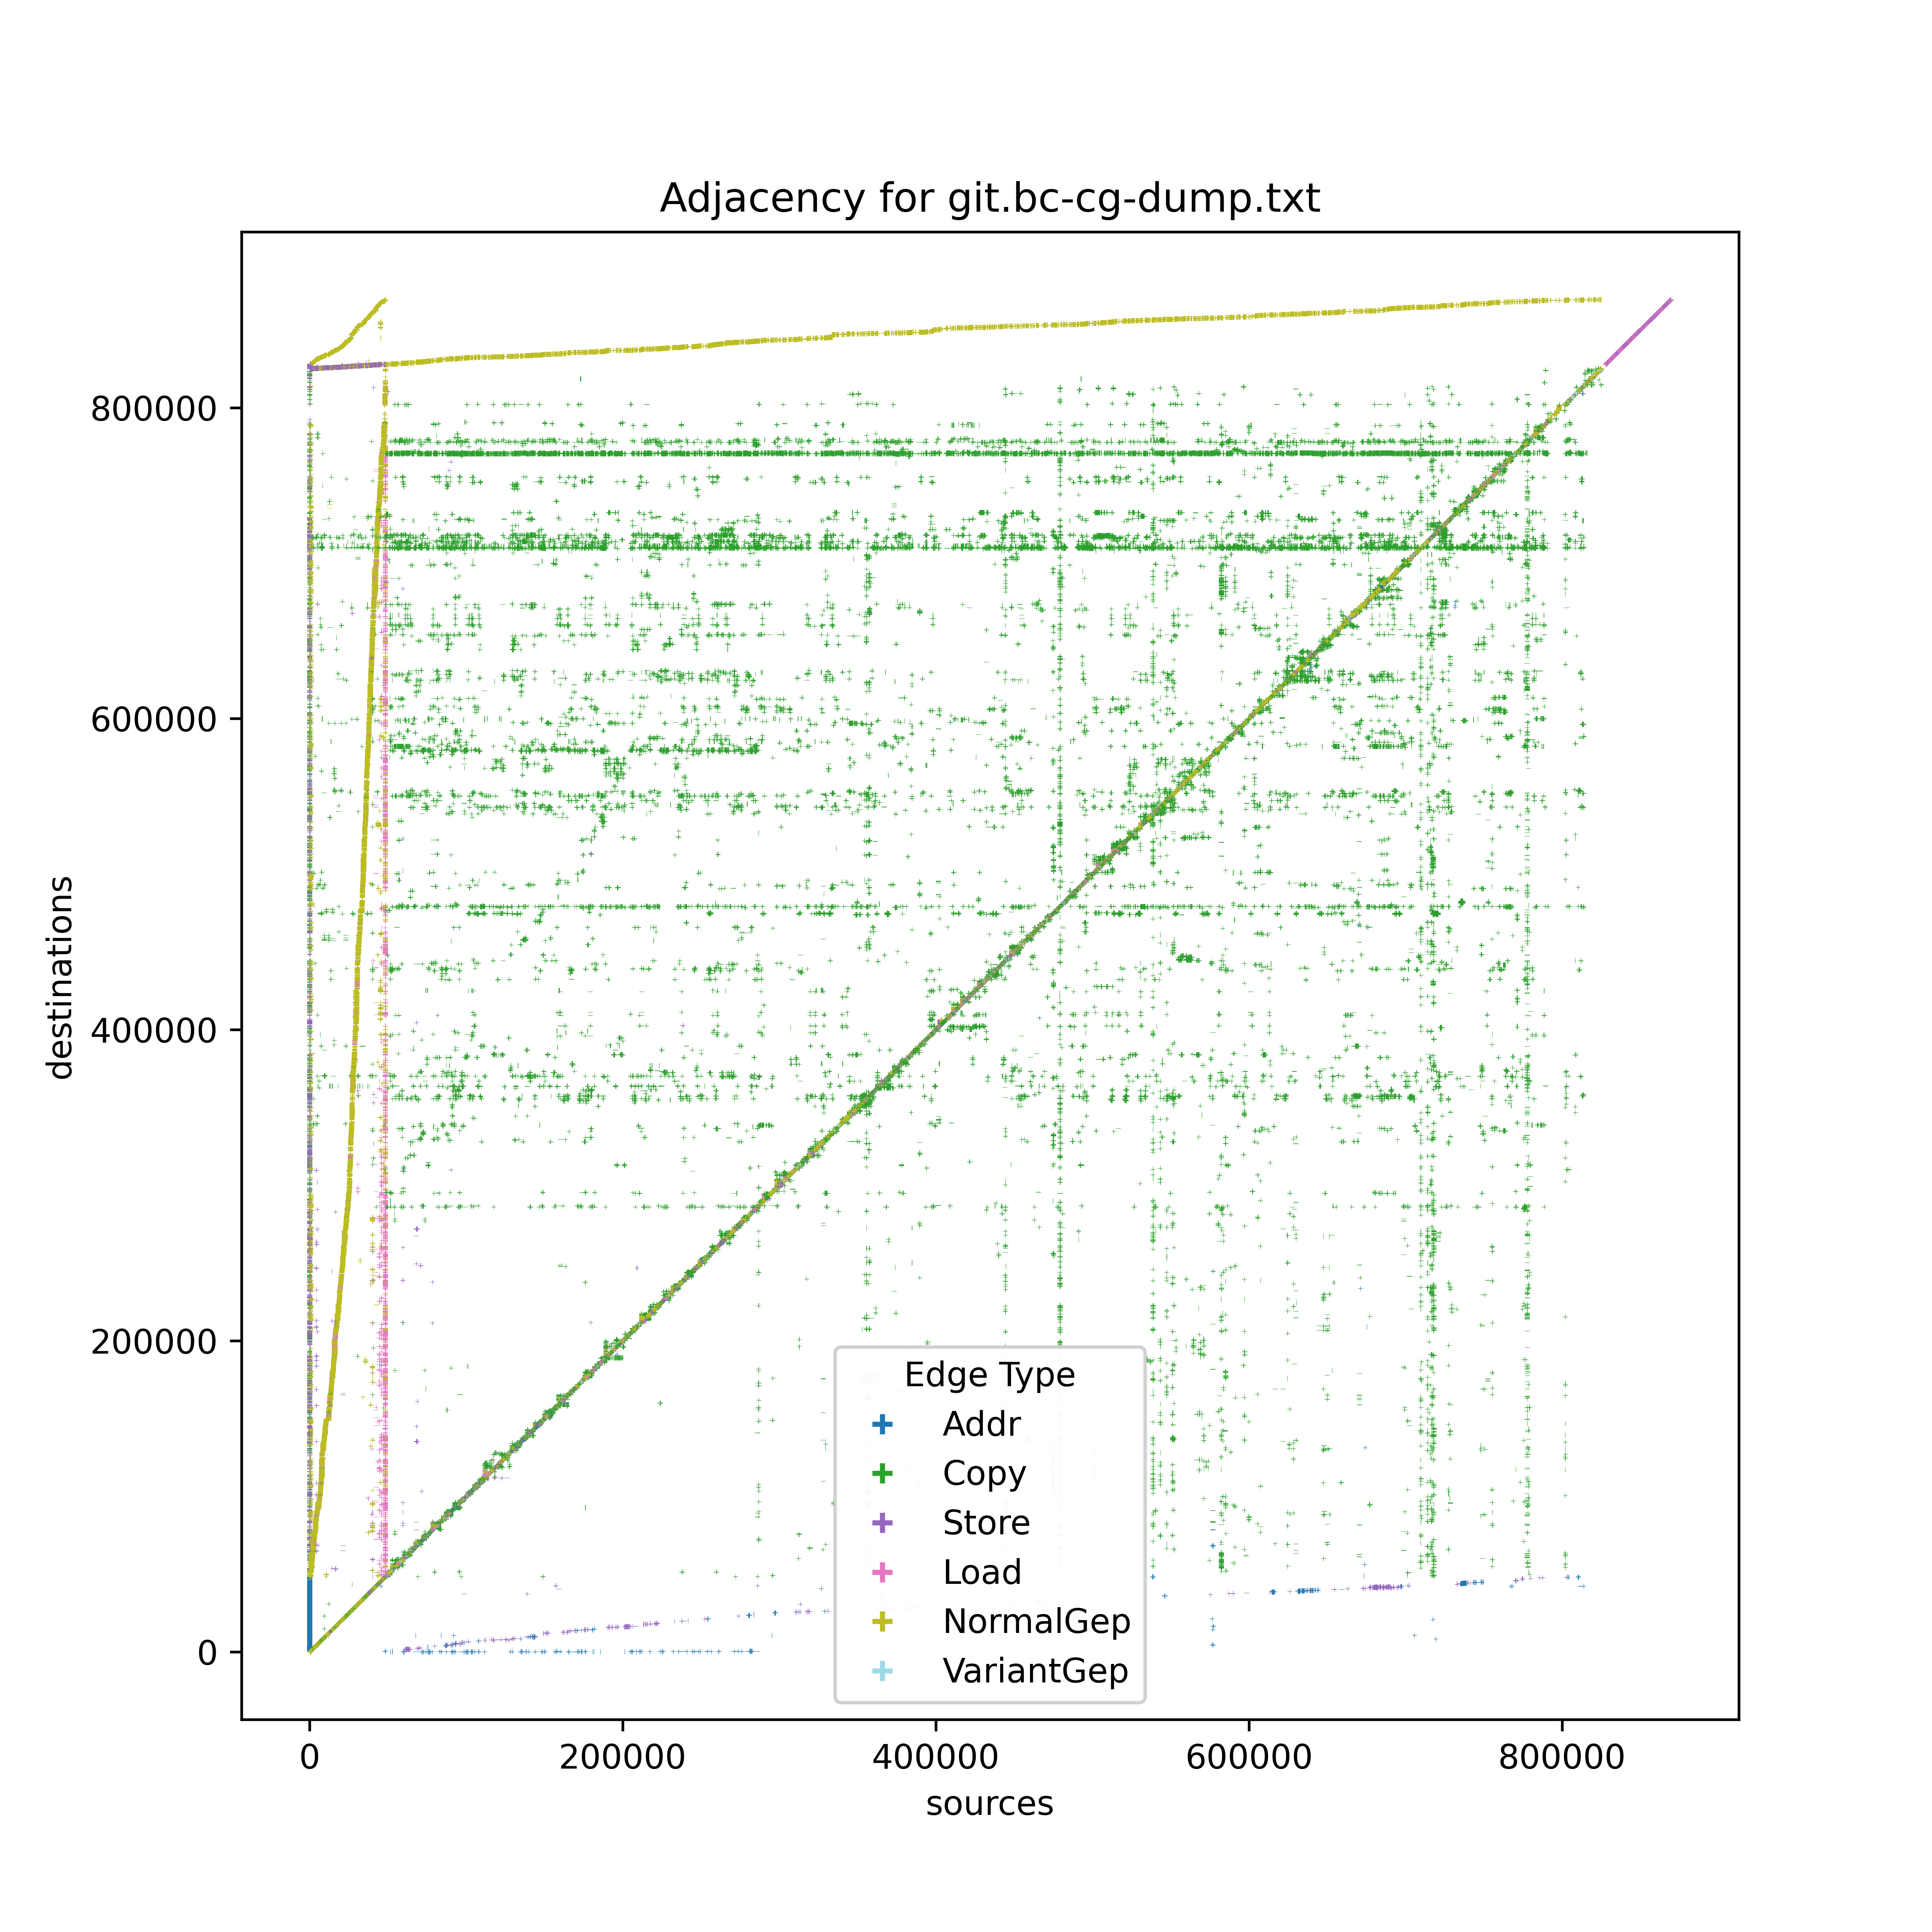
\includegraphics[width=.7\textwidth]{img/plot-git.bc-cg-dump.txt-min.png}
    \caption{Adjacency Plot for the Constraint Graph of the Git Client}
    \label{fig:git-consg}
\end{figure}

\begin{figure}[h]
    \centering
    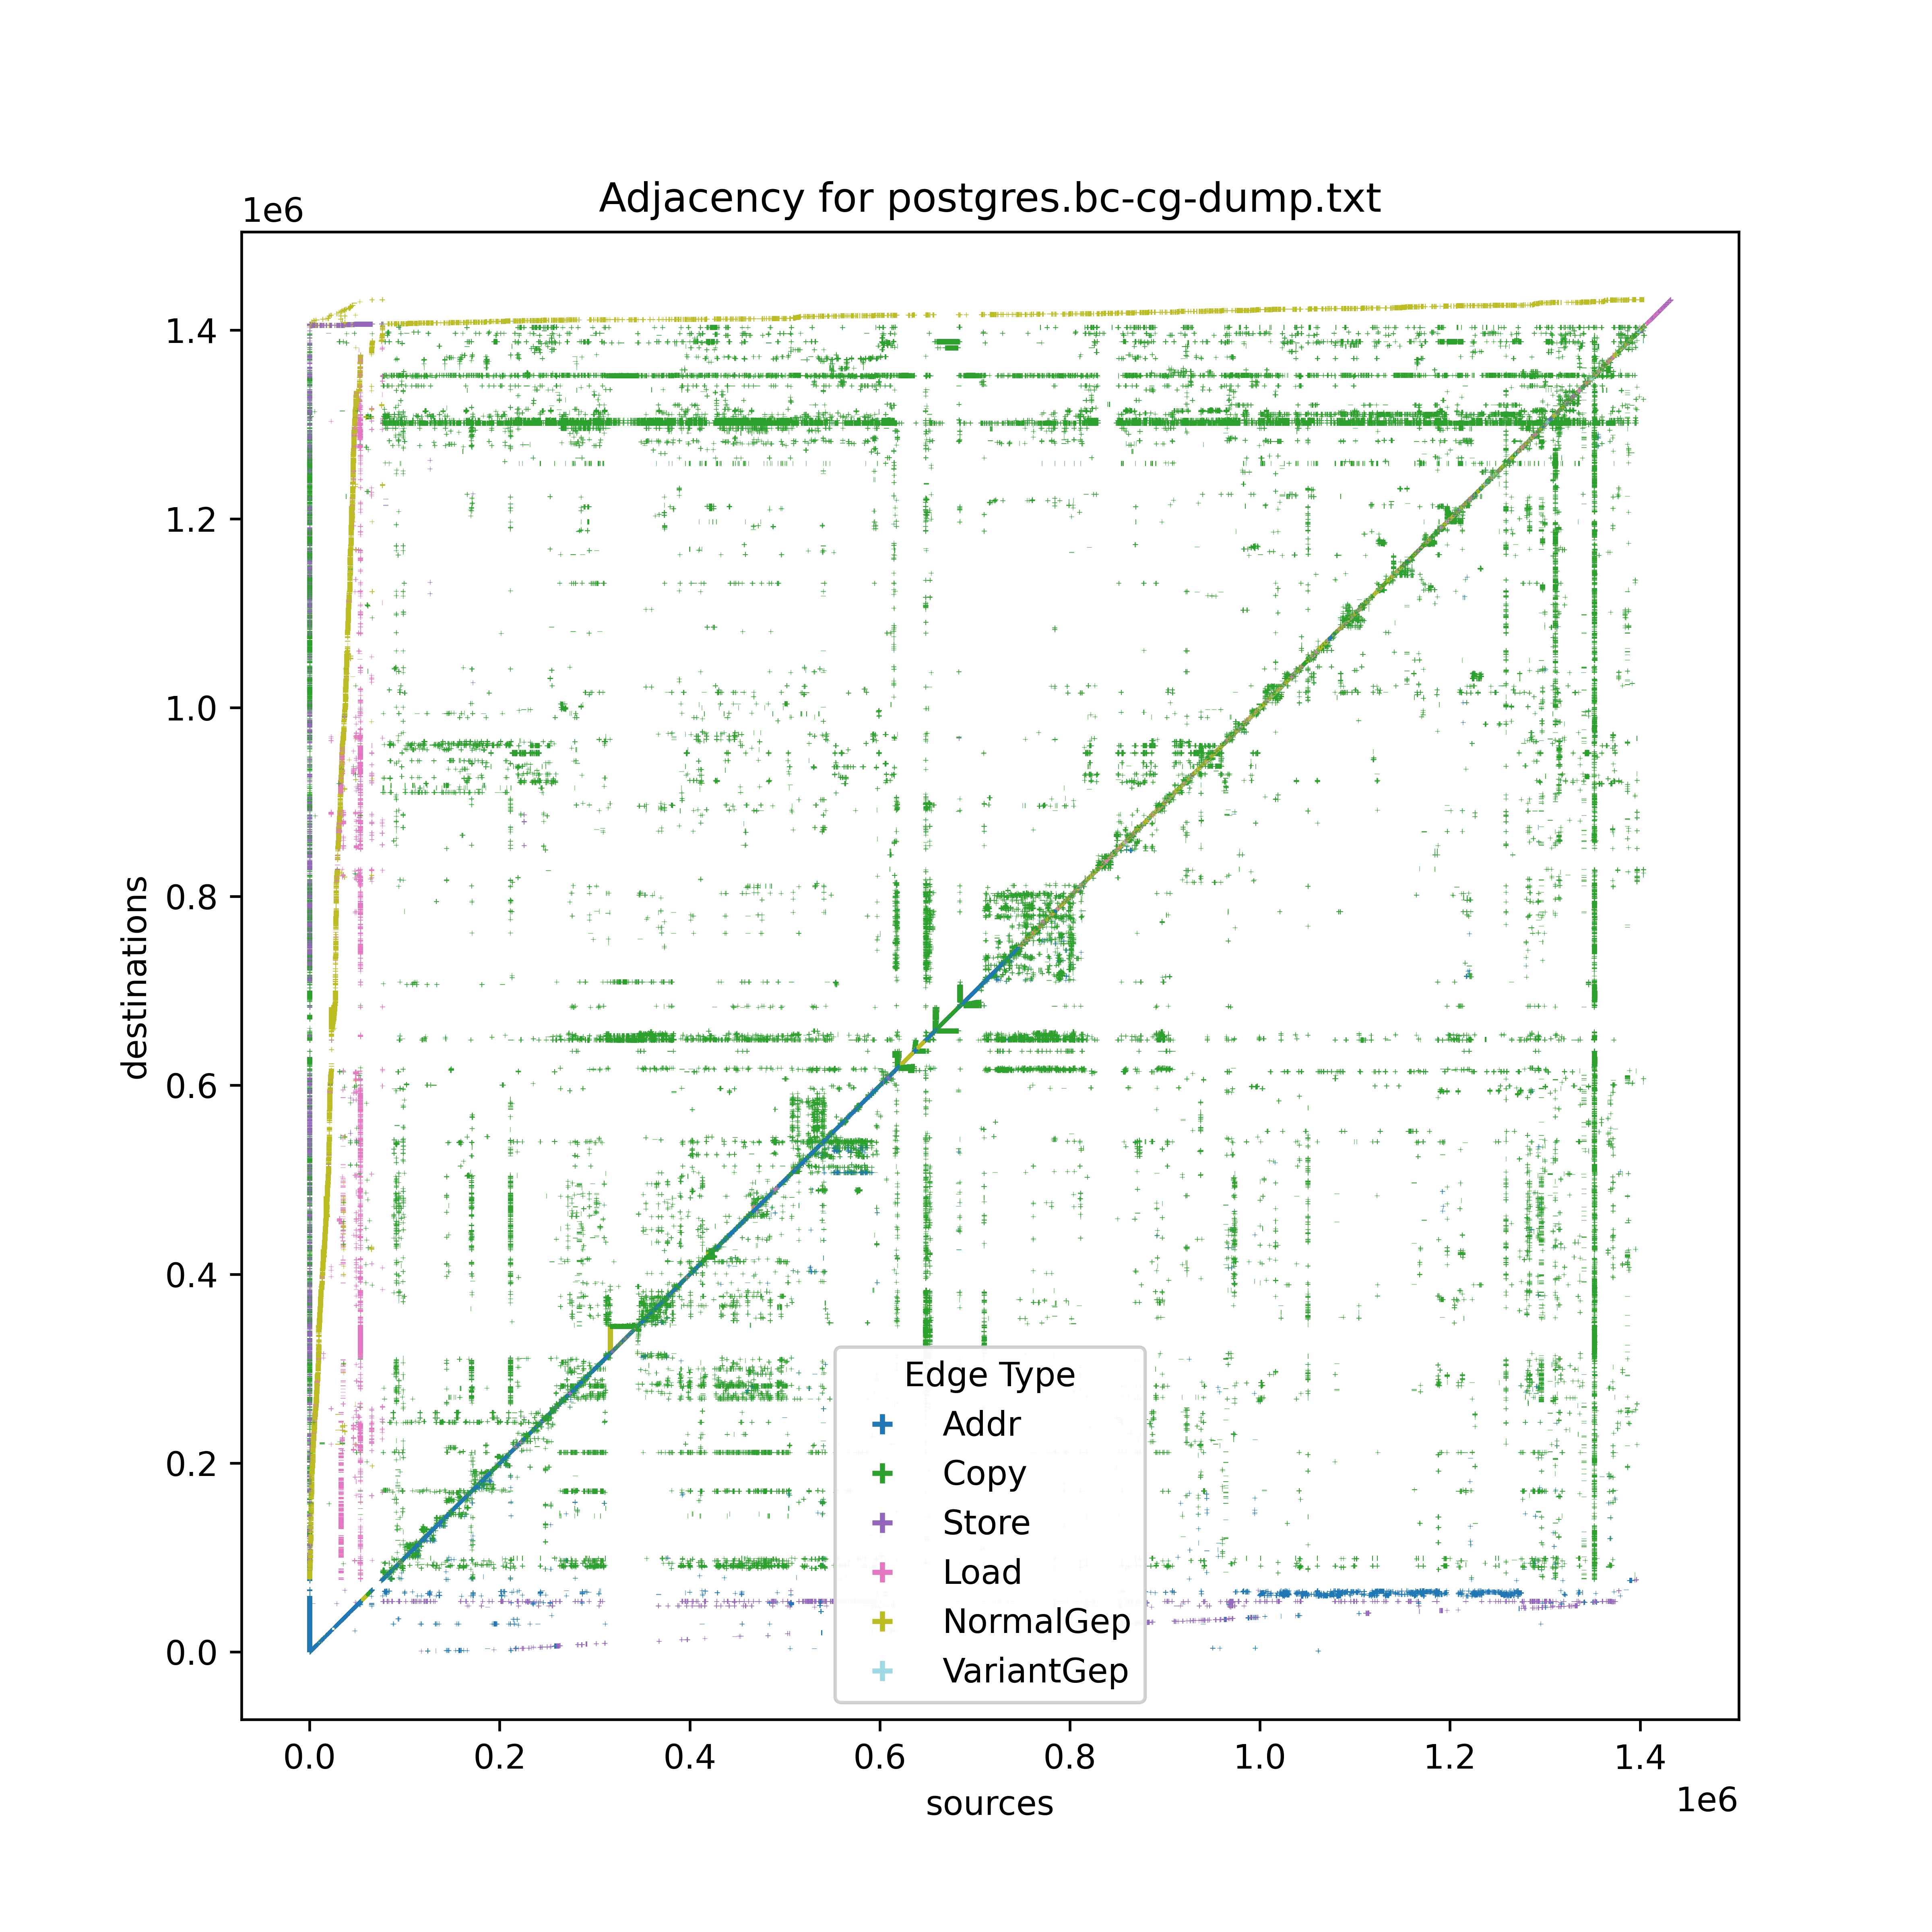
\includegraphics[width=.7\textwidth]{img/plot-postgres.bc-cg-dump.txt-min.png}
    \caption{Adjacency Plot for the Constraint Graph of Postgres}
    \label{fig:postgres-consg}
\end{figure}
\printbibliography[heading=bibintoc]
\end{document}